% COS30049 Assignment 3 -- delivery plan (not the report).
% Group HCMC_COS30049.1_4. Compile with pdfLaTeX three times in this folder:
%   pdflatex main && pdflatex main && pdflatex main
\documentclass[a4paper,11pt]{article}

% ---------------------------------------------------------------- page and fonts
\usepackage[margin=2.3cm]{geometry}
\usepackage[T1]{fontenc}
\usepackage[utf8]{inputenc}
\usepackage{lmodern}
\usepackage{microtype}
\usepackage{parskip}
\setlength{\emergencystretch}{3em} % lets lines with long monospace commands break cleanly
\DeclareUnicodeCharacter{2192}{\ensuremath{\rightarrow}}
\DeclareUnicodeCharacter{2265}{\ensuremath{\geq}}
\DeclareUnicodeCharacter{2264}{\ensuremath{\leq}}
\DeclareUnicodeCharacter{00D7}{\ensuremath{\times}}
\DeclareUnicodeCharacter{2212}{\ensuremath{-}}
\DeclareUnicodeCharacter{2248}{\ensuremath{\approx}}
\DeclareUnicodeCharacter{00F7}{\ensuremath{\div}}
\DeclareUnicodeCharacter{00B1}{\ensuremath{\pm}}

% ---------------------------------------------------------------- tables
\usepackage{array}
\usepackage{booktabs}
\usepackage{tabularx}
\usepackage{longtable}
\usepackage{multirow}
\usepackage{colortbl}
\renewcommand{\arraystretch}{1.22}
\newcolumntype{L}[1]{>{\raggedright\arraybackslash\hspace{0pt}}p{#1}}
\newcolumntype{Y}{>{\raggedright\arraybackslash\hspace{0pt}}X}
\newcolumntype{C}[1]{>{\centering\arraybackslash}p{#1}}

% ---------------------------------------------------------------- figures and drawing
\usepackage{graphicx}
\usepackage{float}
\usepackage{caption}
\captionsetup{font=small, labelfont=bf}
\captionsetup[table]{position=top}
\usepackage{tikz}
\usetikzlibrary{arrows.meta, positioning, calc, fit, backgrounds, shapes.geometric}

% ---------------------------------------------------------------- text
\usepackage{amsmath}
\usepackage{amssymb}
\usepackage{enumitem}
\setlist{itemsep=2pt, topsep=3pt, parsep=0pt}
\usepackage{xcolor}
\usepackage{pifont}
\usepackage{titlesec}
\usepackage{fancyhdr}
\usepackage{url}
\usepackage{listings}
\usepackage[skins,breakable]{tcolorbox}

\definecolor{ink}{HTML}{1F2933}
\definecolor{accent}{HTML}{1D4ED8}
\definecolor{accentsoft}{HTML}{E8EEFC}
\definecolor{okgreen}{HTML}{15803D}
\definecolor{oksoft}{HTML}{E7F5EC}
\definecolor{warn}{HTML}{B45309}
\definecolor{warnsoft}{HTML}{FDF1E3}
\definecolor{grey}{HTML}{6B7280}
\definecolor{greysoft}{HTML}{F3F4F6}
\definecolor{violet}{HTML}{6D28D9}
\definecolor{violetsoft}{HTML}{F1EBFD}
\definecolor{teal}{HTML}{0F766E}
\definecolor{tealsoft}{HTML}{E6F4F2}

\titleformat{\section}{\Large\bfseries\color{ink}}{\thesection}{0.8em}{}
\titleformat{\subsection}{\large\bfseries\color{ink}}{\thesubsection}{0.7em}{}
\titleformat{\subsubsection}{\normalsize\bfseries\color{ink}}{\thesubsubsection}{0.6em}{}
\titlespacing*{\section}{0pt}{1.4em}{0.6em}
\titlespacing*{\subsection}{0pt}{1.1em}{0.4em}

\pagestyle{fancy}
\fancyhf{}
\fancyhead[L]{\small\color{grey}COS30049 A3 delivery plan}
\fancyhead[R]{\small\color{grey}HCMC\_COS30049.1\_4}
\fancyfoot[C]{\small\thepage}
\renewcommand{\headrulewidth}{0.3pt}
\setlength{\headheight}{14pt}

% Boxes. Each one has a single job, so a reader can skim by colour.
\newtcolorbox{decision}[1]{enhanced, breakable, colback=accentsoft, colframe=accent,
  boxrule=0.6pt, arc=2pt, left=6pt, right=6pt, top=4pt, bottom=4pt,
  title={\textbf{Decision:} #1}, fonttitle=\small, coltitle=white}
\newtcolorbox{done}{enhanced, breakable, colback=oksoft, colframe=okgreen,
  boxrule=0.6pt, arc=2pt, left=6pt, right=6pt, top=3pt, bottom=3pt,
  title={\textbf{Done when}}, fonttitle=\small, coltitle=white}
\newtcolorbox{feeds}{enhanced, breakable, colback=violetsoft, colframe=violet,
  boxrule=0.6pt, arc=2pt, left=6pt, right=6pt, top=3pt, bottom=3pt,
  title={\textbf{Feeds the report and rubric}}, fonttitle=\small, coltitle=white}
\newtcolorbox{caution}{enhanced, breakable, colback=warnsoft, colframe=warn,
  boxrule=0.6pt, arc=2pt, left=6pt, right=6pt, top=3pt, bottom=3pt,
  title={\textbf{Watch out}}, fonttitle=\small, coltitle=white}
\newtcolorbox{team}{enhanced, breakable, colback=tealsoft, colframe=teal,
  boxrule=0.6pt, arc=2pt, left=6pt, right=6pt, top=3pt, bottom=3pt,
  title={\textbf{Needs a teammate}}, fonttitle=\small, coltitle=white}
\newtcolorbox{summarybox}{enhanced, breakable, colback=greysoft, colframe=ink,
  boxrule=0.6pt, arc=2pt, left=8pt, right=8pt, top=6pt, bottom=6pt,
  before upper={\setlength{\parskip}{0.5em}}}

% Command and JSON blocks. Plain monospace; no shell-escape needed.
\lstdefinestyle{cmd}{basicstyle=\ttfamily\small, backgroundcolor=\color{greysoft},
  frame=single, framerule=0pt, xleftmargin=4pt, xrightmargin=4pt, aboveskip=6pt,
  belowskip=6pt, columns=fullflexible, keepspaces=true, breaklines=true,
  showstringspaces=false, upquote=true}
\lstdefinestyle{json}{style=cmd, basicstyle=\ttfamily\footnotesize}
\lstdefinestyle{py}{style=cmd, language=Python, keywordstyle=\color{accent}\bfseries,
  commentstyle=\color{grey}\itshape, stringstyle=\color{okgreen}}
\lstset{style=cmd}

\newcommand{\code}[1]{\texttt{\detokenize{#1}}}
\newcommand{\fp}[1]{\path{#1}} % file paths, breakable at / and .
\newcommand{\yes}{\textcolor{okgreen}{\ding{51}}}
\newcommand{\no}{\textcolor{warn}{\ding{55}}}
\newcommand{\est}{\textsuperscript{\textcolor{grey}{est.}}}
% Scope tiers, as coloured tags.
\newcommand{\must}{\textcolor{accent}{\textbf{Must}}}
\newcommand{\should}{\textcolor{teal}{\textbf{Should}}}
\newcommand{\could}{\textcolor{violet}{\textbf{Could}}}
\newcommand{\wont}{\textcolor{grey}{\textbf{Won't}}}

\usepackage[hidelinks]{hyperref}
\hypersetup{colorlinks=true, linkcolor=accent, urlcolor=accent, citecolor=accent}

\begin{document}

% ---------------------------------------------------------------- title page
\begin{titlepage}
\thispagestyle{empty}
\vspace*{1.2cm}
{\color{grey}\large COS30049 Computing Technology Innovation Project}\par
\vspace{0.4cm}
{\color{ink}\Huge\bfseries Assignment 3 delivery plan}\par
\vspace{0.3cm}
{\color{ink}\Large The web application: its scope, its interfaces and the work to build,\\ test, document and submit it between 10 November and 6 December 2026}\par
\vspace{1.0cm}
\begin{tabularx}{\textwidth}{@{}L{4.2cm}Y@{}}
\toprule
Project & Bitcoin Address Activity Explorer: a React and FastAPI application on Assignment 2's models (an unusual-activity indicator, never a fraud verdict) \\
Group & HCMC\_COS30049.1\_4 \\
Members & Cam Dan Bui (105967074); Cao Tri Tran (106214726); Le Quang Anh Hoang (106218605); Minh Khang Nguyen (106216803) \\
Tutor & Arthur Hoang \\
Plan prepared & Tuesday 10 November 2026 (teaching Week 9, day 57 of the 84-day unit) \\
Assignment 3 due & Sunday 6 December 2026, 23:59 GMT+7 (day 83; the brief says ``Sunday, Week 12''); 26 days from this plan \\
Planned submission & Saturday 5 December 2026, one day early \\
Weight & 45\% of the unit (45 points); hurdle of 40\% in every assignment \\
Machines & PC: Windows 11, Intel Core i5-12600K, 16 GB. Mac: Apple M5, 16 GB. No GPU is needed \\
\bottomrule
\end{tabularx}

\vspace{0.8cm}
\begin{summarybox}
\textbf{What this document is.} A working plan and a scope specification for Assignment 3. It
fixes what the application does and does not do, screen by screen, endpoint by endpoint and chart by
chart, so that building it later is a matter of following numbered items. It also says how each item
is checked, who owns it, when it is due and which rubric line it earns.

\textbf{What it is not.} It is not the report and is not submitted. Numbers marked \est{} are
planning estimates that a measured run replaces. Timings without that mark were measured on the Mac
on 10 November 2026 with Assignment 2's code at commit \code{aa56a26}.

\textbf{What needs the team first.} Three items block the work and are listed in
Section~\ref{sec:needsteam}: the tutor's answer on generative AI for this assignment, the approval
of change requests CR-07 and CR-08, and the split of work packages between the four members.
\end{summarybox}
\vfill
{\small\color{grey}Source documents read for this plan: the Assignment 3 brief and rubric as
transcribed into \fp{docs/brief/}; the submitted Assignment 1 report (requirements, planned API,
WBS 1.4, risk register, prototype design); the prototype repository (commit \code{8375cf0}); the
Assignment 2 repository at commit \code{aa56a26} (\code{explorer/predict.py}, \code{explore.py},
\code{settings.json}, README, delivery plan, change log); and the Week 8 lecture and workshop. The
Week 9--12 material was not yet available, so the stack choices in Section~\ref{sec:decisions}
are checked against it when it is released.}
\end{titlepage}

\tableofcontents
\clearpage

\section{The plan on one page}
\label{sec:summary}

\textbf{Goal.} A full-marks attempt at all 45 points and at every line of the brief's High
Distinction list. Every item in this plan is tied to a rubric line, a line of the brief, or a
promise made in Assignment 1 or 2. An item that earns none of these was left out.

\textbf{The marks, from the rubric.}

\begin{center}
\small
\begin{tabularx}{\textwidth}{@{}Y C{0.9cm} Y C{0.9cm}@{}}
\toprule
\textbf{Functionality} & \textbf{18} & \textbf{Visualisation} & \textbf{11} \\
\midrule
1. AI model integration & 3 & 1. Chart diversity and relevance (three or more types) & 3 \\
2. Front-end and back-end communication & 4 & 2. Interactivity (zoom, filtering, tooltips, updates) & 4 \\
3. Error handling and input validation & 3 & 3. Clarity (labels, legends, titles, units) & 2 \\
4. Back-end API design (REST, two or more methods) & 4 & 4. Performance and loading & 2 \\
5. Real-time updates and responsiveness & 4 & & \\
\midrule
\textbf{Source code} & \textbf{5} & \textbf{Usability} & \textbf{6} \\
\midrule
1. Execution (no errors or warnings, quick start) & 2 & 1. User interface (responsive, advanced components) & 3 \\
2. Comments & 1 & 2. User experience (feedback, personal touches, transitions) & 3 \\
3. Code structure & 2 & & \\
\midrule
\textbf{Report} (PDF, 8 pages at most) & \textbf{5} & & \\
\midrule
1. Formatting and Harvard referencing & 1 & 3. API endpoint documentation & 2 \\
2. System architecture and implementation & 2 & & \\
\bottomrule
\end{tabularx}
\end{center}

Forty of the 45 points are judged from the running application, and the brief says a video that
cannot be opened scores zero for most components. The application and its demonstration video
therefore come first; the report is five points.

\textbf{What will be built.}
\begin{enumerate}
  \item \textbf{A FastAPI back end around Assignment 2's \code{Predictor}.} It keeps the five
    endpoints Assignment 1 planned, with the same JSON, and adds a what-if prediction, a response
    curve, exports, a method list, a health check and the settings the front end needs
    (Section~\ref{sec:api}). Eleven endpoints are Must; eleven more come with the Should and Could
    items.
  \item \textbf{The React front end, grown from the Assignment 1 prototype.} Its three screens move
    from illustrative data to the real snapshot of 28 addresses and 7,966 transactions. Five views
    are added: a what-if lab, a models and limits page, a watchlist, an about page and a live-lookup
    dialog (Section~\ref{sec:frontend}).
  \item \textbf{User input to prediction in real time.} A validated form takes a hypothetical
    transaction (amount, direction, time) and shows every model's verdict as the user types. One
    request scores a whole range of amounts: measured at 0.16 s for seven amounts, identical to
    seven single calls that took 1.88 s (Section~\ref{sec:model}).
  \item \textbf{Interactive charts in Plotly.js.} Four are Must and cover three chart types (bar,
    scatter, line); two more are Should; three are Could (Section~\ref{sec:charts}). Each has zoom,
    tooltips, a legend, units, the snapshot date, a table view and an export.
  \item \textbf{Validation and error handling on both tiers}, from one table of rules and one
    catalogue of states (Section~\ref{sec:errors}).
  \item \textbf{The High Distinction features}: a method selector, a watchlist with notes, the
    guarded Explorer Assistant, a replay of an address's history, and a live lookup of any Bitcoin
    address, which needs change request CR-08.
  \item \textbf{The submission}: the report (8 pages), the code zip with its README, the video
    (7 minutes), the minutes for Weeks 1 to 12 and the contribution form (Section~\ref{sec:report}).
\end{enumerate}

\textbf{How this keeps the earlier promises.} Assignment 1's success measure was that AC-01 to
AC-03 and FR-05 pass on every snapshot address in the Assignment 3 build and are shown in the video.
That is milestone MS2. The wording rule does not change: the application says ``unusual'', ``flag''
and ``worth a look'', and every flagged item carries the line \emph{``Unusual activity requires
investigation; it does not indicate wrongdoing.''} Assignment 2's numbers are not touched: the
models are loaded as they were frozen at \code{results-v1.1}.

\textbf{The dates that matter.}
\begin{center}
\small
\begin{tabularx}{\textwidth}{@{}L{3.2cm}Y@{}}
\toprule
\textbf{Date} & \textbf{Milestone} \\
\midrule
Wed 11 Nov & CR-07 and CR-08 sent to the team; the questions in Appendix~\ref{app:cr} sent to the tutor. \\
Sun 15 Nov & MS1, the walking skeleton: the five Assignment 1 endpoints answer from the real snapshot and the three prototype screens show them. \\
Sun 22 Nov & MS2, the Must tier: the minimum viable demonstration passes on all 28 addresses, with the what-if lab, four charts, validation, error states and export. \\
Fri 27 Nov & MS3, feature freeze: the Should items that are finished stay; the rest are cut and recorded. \\
Sun 29 Nov & MS4, code freeze: a teammate installs from the README on Windows and on macOS; tag \code{v1.0-rc}. \\
Sat 5 Dec & MS5: everything submitted on Canvas. Sunday 6 December is spare. \\
\bottomrule
\end{tabularx}
\end{center}

\textbf{The critical path.} API contract → back-end endpoints → front end on the real API →
what-if and charts → MS2 → usability walkthrough and fixes → clean install → video → submission.
The Should items hang off MS2 and are never on this path. Assignment 1's baseline started this work
on about 28 October; it starts on 10 November, so 34 planned days are done in 26. Section
\ref{sec:schedule} shows how, and Section~\ref{sec:cutorder} says what is cut first.

\subsection{What needs the team this week}
\label{sec:needsteam}

\begin{team}
\begin{enumerate}
  \item \textbf{Generative AI (the tutor).} The brief says generative AI ``must not be used to
    generate content for this assignment'', allows it for learning, idea generation and debugging,
    and requires all use to be acknowledged in the report. For Assignment 2 the tutor allowed AI on
    condition of a separate declaration. Ask Arthur Hoang by Wed 11 Nov whether that arrangement
    covers Assignment 3, and build nothing that depends on the answer before it arrives
    (risk 32). The use log continues in \fp{docs/AI_USE_LOG.md} either way.
  \item \textbf{CR-07 and CR-08 (all four members).} Assignment 1's change control needs every
    member's recorded agreement to add the optional items and to allow a live lookup
    (Appendix~\ref{app:cr}).
  \item \textbf{Owners (weekly meeting, Week 9).} Section~\ref{sec:wp} proposes owners from
    Assignment 1's WBS. Each member needs an area they build and can explain in the video and to the
    tutor. Check the split against the contribution form's scaling rule before anyone starts.
  \item \textbf{Which commit was submitted for Assignment 2 (Cao Tri Tran).} The repository has no
    \code{v1.0} tag. Tag the submitted commit so the back end can name the exact models it loads.
  \item \textbf{The Week 9--12 slides (anyone).} Put them in the shared folder when they are
    released; decisions D-A3-2 to D-A3-4 are checked against them.
\end{enumerate}
\end{team}

\section{What must be submitted, and what earns each mark}
\label{sec:deliverables}

\subsection{The five files}

One member uploads all of them through the ``Assignment 3 Submission'' link. The brief deducts marks
for wrong file names, so the names below follow the group-name pattern used for Assignments 1 and 2.

{\small
\begin{longtable}{@{}L{2.5cm}L{5.3cm}L{4.9cm}L{2.3cm}@{}}
\toprule
\textbf{Deliverable} & \textbf{File} & \textbf{Limits and contents} & \textbf{Owner} \\
\midrule
\endhead
Project report & \fp{HCMC_COS30049.1_4_Assignment3_Report.pdf} & 8 pages at most, not counting the cover, contents, bibliography and appendix. The sections of Section~\ref{sec:reportoutline}; the video link on the cover & Cam Dan Bui integrates; every member writes a part \\
Source code & \fp{HCMC_COS30049.1_4_Assignment3_Code.zip} & \fp{frontend/} without \fp{node_modules}; \fp{backend/} with the model code and the models; \fp{README.md} & Le Quang Anh Hoang; Cao Tri Tran for the models \\
Demonstration video & \fp{HCMC_COS30049.1_4_Assignment3_Video.mp4} & 7 minutes at most; MP4 or AVI; everything in Section~\ref{sec:video} & Minh Khang Nguyen records; all speak \\
Video link, if the file is too large for Canvas & \fp{HCMC_COS30049.1_4-video-link.txt} & An unlisted YouTube link that opens in a private window; the same link on the report's cover & Le Quang Anh Hoang \\
Meeting minutes & \fp{HCMC_COS30049.1_4_Assignment3_Meeting_Minutes.pdf} & One meeting for every week since the team formed: Weeks 1 to 12 & Cam Dan Bui \\
Contribution form & \fp{HCMC_COS30049.1_4_Assignment3_Contribution_Form.pdf} & Each member's details and contribution, signed & All \\
\bottomrule
\end{longtable}
}

\subsection{Rubric line by line}
\label{sec:rubricmap}

The middle column is the rubric's own description of full points. The last column names the scope
items (Section~\ref{sec:scopetable}) that earn it.

{\small
\begin{longtable}{@{}L{3.3cm}C{0.7cm}L{5.6cm}L{4.4cm}@{}}
\toprule
\textbf{Criterion} & \textbf{Pts} & \textbf{Full points mean} & \textbf{Earned by} \\
\midrule
\endhead
Report 1: formatting and referencing & 1 & Professional cover with title, group and student details; tidy layout; Harvard references & M-16; Section~\ref{sec:reportoutline} \\
Report 2: architecture and implementation & 2 & Detailed architecture; implementation described with the reasons for each technology; clear diagrams & M-16; the diagrams of Section~\ref{sec:architecture} \\
Report 3: API documentation & 2 & Every endpoint documented with request type, parameters, JSON structure and examples & M-16; generated from the OpenAPI schema (Section~\ref{sec:api}) \\
Code 1: execution & 2 & No errors or warnings; every feature runs; quick start; dependencies managed & M-01, M-14; Section~\ref{sec:readme} \\
Code 2: comments & 1 & Significant sections explained & M-14; Section~\ref{sec:coderules} \\
Code 3: structure & 2 & Clear hierarchy; modular; best practices & M-01, M-05; Section~\ref{sec:layout} \\
Functionality 1: AI model integration & 3 & Seamless; real-time predictions; handles various input types & M-02, M-03, M-04, M-13; S-01, S-05, S-09 \\
Functionality 2: front-end and back-end communication & 4 & Smooth, error-free GET and POST; prompt; full retrieval and submission & M-02, M-05, M-06, M-11 \\
Functionality 3: error handling and validation & 3 & Every input validated on both tiers; graceful errors with clear messages; invalid data never processed & M-09, M-10 \\
Functionality 4: API design & 4 & RESTful; efficient; two or more HTTP methods used properly; documented; reliable & M-01, M-02, M-03, M-12; S-04 adds PUT and DELETE \\
Functionality 5: real-time updates and responsiveness & 4 & Elements and charts update without delay; performance holds across devices & M-11; S-06, S-09 \\
Visualisation 1: diversity and relevance & 3 & Three or more diverse chart types that suit the data and explain the model's output & M-07 (bar, scatter, line); S-02, S-03 \\
Visualisation 2: interactivity & 4 & Zoom, filtering, tooltips, real-time updates; smooth & M-07, M-08; S-06, S-07 \\
Visualisation 3: clarity & 2 & Predictions easy to read; labels, legends, titles and units & M-07; the chart contract (Section~\ref{sec:chartcontract}) \\
Visualisation 4: performance and loading & 2 & Quick to load and smooth with large data & M-07; S-12; Section~\ref{sec:budgets} \\
Usability 1: user interface & 3 & Polished and responsive; intuitive navigation; advanced components such as modals and dynamic forms & M-05, M-06; Section~\ref{sec:components} \\
Usability 2: user experience & 3 & Feedback mechanisms, personalised interactions and smooth transitions & M-10, M-11, M-15; S-04 \\
\bottomrule
\end{longtable}
}

\subsection{The High Distinction list}
\label{sec:hdmap}

The brief asks for three or more chart types, interactive charts and ``at least three advanced
functionalities'', and gives five examples. The plan covers all five, and three of them are met by
Must items alone.

\begin{center}
\small
\begin{tabularx}{\textwidth}{@{}L{4.6cm}Y L{2.4cm}@{}}
\toprule
\textbf{The brief's example} & \textbf{What the Explorer does} & \textbf{Items} \\
\midrule
Enhanced visualisations: three or more chart types with zoom and filtering, in D3.js or Plotly.js & Bar, scatter and line charts in Plotly.js with zoom, pan, a range slider, tooltips, a filter bar and click-through; a dot chart and a grouped bar chart added & M-07, M-08; S-02, S-03, S-07 \\
Real-time updates: live data feeds or auto-refreshing charts & The what-if verdict and curve refresh as the user types; a replay feeds an address's history to the charts; a live lookup streams its progress & M-11; S-06; S-09 \\
Custom user input: advanced forms, full validation, dynamic feedback & The what-if form: amount with a unit switch and a slider, direction, time; rules checked on each keystroke and again on the server & M-06, M-09 \\
Error handling: robust, with clear messages on both ends & One error body, one catalogue of states, a next action on every state & M-10 \\
User-experience extras: export of predictions and charts & CSV and JSON of scored transactions; PNG of every chart; a scenario table & M-12; S-08 \\
\bottomrule
\end{tabularx}
\end{center}

\subsection{Promises from Assignments 1 and 2 that this build must keep}
\label{sec:promises}

{\small
\begin{longtable}{@{}L{5.4cm}L{2.6cm}L{6.0cm}@{}}
\toprule
\textbf{Promise} & \textbf{Where made} & \textbf{How Assignment 3 keeps it} \\
\midrule
\endhead
FR-01 to FR-05: select a supported address; timeline; drilldown; a reason, a comparison basis and the limitation line on every flag; five distinguishable feedback states & A1 Table 2.1 & Views V1 to V3 on the real API; journeys J1 to J3; acceptance tests AT-01 to AT-05 \\
AC-01 to AC-03 and FR-05 pass on every snapshot address and are shown in the video & A1 §1.1 & MS2 runs them on all 28 addresses automatically; the video shows them on one \\
The five planned endpoints, with 400, 404 and 422 & A1 Table 2.7 & E3 to E7 keep their paths, methods and bodies (Section~\ref{sec:api}) \\
The screens move to real data ``without changing screen code'' & A1 §10 & The API client is swapped; screen components change only where a view gains a feature \\
NFR-01: units, source and snapshot date on every chart; the limitation line; none of the five banned words; two walkthrough participants read a flag as ``needs investigation'' & A1 Table 2.5 & The chart contract; the wording test on both tiers; the walkthrough (M-15) \\
NFR-03: keyboard navigation, visible focus, contrast, recovery from mistakes & A1 Table 2.5 & Section~\ref{sec:a11y}; the timeline chart keeps its arrow-key control \\
Charts in Plotly.js; the API called with Axios & A1 WBS dictionary, 1.4.3 and 1.4.4 & D-A3-3 and D-A3-4 \\
The three issues of the heuristic inspection: z-scores may confuse; the unusual-days list hides its overflow; the prototype tools cover content & A1 Table 10.2 & Plain words first, z in the table and tooltip; a ``Show all'' control; the tools removed from the build \\
Optional items go through change control; no live blockchain calls from the application & A1 §2.6, §8.5, WBS 1.4.5 & CR-07 and CR-08 (Appendix~\ref{app:cr}); the Must tier never needs the network \\
The integrated product shows the model evaluation and its known limitations & A1 §9 & View V5, models and limits (M-13) \\
The usability walkthrough, moved to ``the Assignment 3 usability study'' & A2 report, objectives table & M-15, in Week 11, with Assignment 1's four tasks and observer sheet \\
\code{predict.py} is the interface the back end wraps; the Assistant is optional and off by default; Assignment 2's numbers do not change & A2 plan §15 & Section~\ref{sec:model}; S-05; W-06 \\
A post-project review of what changed and what the team learned & A1 §9 & Week 12 minutes (Section~\ref{sec:minutes}) \\
\bottomrule
\end{longtable}
}

\subsection{Rules in the brief that are easy to miss}

\begin{itemize}
  \item \textbf{The video carries the marks.} If it cannot be opened when marking happens, most
    components score zero. It must show desktop, tablet and mobile sizes, every interaction, the
    whole path from input to chart, and the key technical decisions and difficulties.
  \item \textbf{The report documents at least four endpoints} and must describe preprocessing,
    postprocessing, error handling, validation and any change made to the model for the web.
  \item \textbf{The zip holds the model code} that the web application uses, with its
    modifications, and a README that covers set-up, libraries, how to run both tiers and how the
    model is configured.
  \item \textbf{Generative AI}: see Section~\ref{sec:needsteam}, item 1. All use is acknowledged
    in the report.
  \item \textbf{Late work} loses 10\% of the available mark per day and scores zero after seven days.
  \item \textbf{Nothing about the work is posted publicly} on Canvas discussions. The GitHub
    repository for Assignment 2 is public; decision D-A3-1 keeps the Assignment 3 repository
    private until marks are released.
\end{itemize}

\section{Where we start}
\label{sec:start}

Two finished pieces already fit together: Assignment 2's prediction module returns the JSON shapes
that Assignment 1's prototype screens read. Assignment 3 is the layer between them and the features
around them.

\subsection{From Assignment 2: the models and \code{predict.py}}
\label{sec:inherited}

\code{Predictor.load()} reads the saved artefacts once; every method returns plain dictionaries in
camelCase. The timings are from the Mac (Apple M5, CPU environment \code{cos30049-a2}) on
10 November 2026.

{\small
\begin{longtable}{@{}L{4.9cm}L{5.8cm}L{3.3cm}@{}}
\toprule
\textbf{Function} & \textbf{Returns} & \textbf{Measured} \\
\midrule
\endhead
Import and \code{Predictor.load()} & Features, transactions and scores of the snapshot; nine saved methods; the selected method & 4.7 s to import, 0.9 s to load \\
\code{score_address(address)} & Snapshot, range, per-day counts, totals, history status and every transaction's full detail & 0.04 s (273 transactions) to 0.10 s (700); 0.8 to 2.0 MB of JSON \\
\code{transaction(address, txid)} & One transaction's detail & as above (it scores the address) \\
\code{score_what_if(address, amount_btc, direction, time_utc)} & A hypothetical transaction scored against the real, strictly earlier history by eight methods & 0.40 s \\
The same, for many amounts in one feature build & Identical scores for all eight methods & 7 amounts: 0.16 s, against 1.88 s for seven single calls. 41 amounts: 0.18 s \\
\code{explain(tx, use_assistant)} & The template text, or the first Assistant answer that passes the guardrail & under 1 ms for the template; about 10 s for the Assistant on the PC's CPU (README), after a first load of up to a minute \\
\code{txgpt_surprisal(address)} & Surprisal per transaction and per field, from a saved table & a table read \\
\code{classify_heist}, \code{classify_elliptic} & The labelled-data classifiers & not used (W-04) \\
\bottomrule
\end{longtable}
}

\textbf{The data behind them.} The snapshot of 22 October 2026 holds 28 addresses (25 main and 3
with too little history to score) and 7,966 transactions; the largest address has 700 and the
smallest 3. The Explorer's flags come from the robust-z baseline, which flags a transaction when any
feature's $|z|$ reaches 5.0. Nine methods have a saved model and a threshold
(Section~\ref{sec:methods}). \code{Unsupported} and \code{InsufficientHistory} are the exceptions
behind Assignment 1's 404 and 422.

\textbf{What the running example looks like.} Address
\code{1Bbcsfxj2JRUD5crcdZVHBcViT61vrJ3dz} has 377 transactions on 214 days from 16 May 2024 to
19 October 2026; 367 are scored and 3 are flagged, on 3 days. A what-if of 0.05 BTC out at
\code{2026-10-20T12:00:00Z} is flagged with score 5.98: 0.05 BTC against a usual 0.000525 BTC. The
plan uses this address in every example, as Assignment 2's README does.

\subsection{From Assignment 1: the prototype}

\begin{itemize}
  \item A React and TypeScript application built with Vite (\fp{asm1_demo/frontend}, commit
    \code{8375cf0}): about 4,800 lines, 66 tests.
  \item Three linked screens: address selection, daily timeline, day and transaction detail.
  \item Six feedback states, each with a next action: invalid, unsupported, loading, empty,
    insufficient history and network failure.
  \item A hash router, so every screen and state has its own link and the back button works.
  \item Address validation in the browser with the real checksums (Base58Check, Bech32, Bech32m).
  \item \fp{src/api/types.ts}, the contract, and \fp{src/api/http.ts}, a client for the planned
    back end that is switched on with \code{VITE_API_MODE=http}. A mock answers the same five
    endpoints in the browser.
  \item Two charts drawn by hand in SVG, keyboard control of the timeline, a table view of each
    chart, light and dark themes, layouts checked at 1280, 820 and 390 pixels by a screenshot script
    that fails on sideways scrolling.
\end{itemize}

\subsection{The gaps Assignment 3 closes}
\label{sec:gaps}

\begin{center}
\small
\begin{tabularx}{\textwidth}{@{}L{5.2cm}Y L{2.0cm}@{}}
\toprule
\textbf{Today} & \textbf{Needed} & \textbf{Section} \\
\midrule
No server: \code{predict.py} is called from a terminal & A FastAPI service with routes, schemas, validation, errors and documentation & \ref{sec:architecture}, \ref{sec:api} \\
\code{score_address} returns up to 2 MB at once & Small responses per view: timeline, a page of rows, one detail & \ref{sec:api} \\
The prototype shows invented data & The same screens on the real snapshot & \ref{sec:frontend} \\
No form sends user input to a model & The what-if lab, validated on both tiers & \ref{sec:viewwhatif}, \ref{sec:errors} \\
Charts are hand-drawn SVG, two types, no zoom & Plotly.js charts, three or more types, zoom, filters, export & \ref{sec:charts} \\
Nothing updates by itself & Live what-if, replay, live-lookup progress & \ref{sec:realtime} \\
No export, no personal state & CSV, JSON and PNG export; watchlist and preferences & \ref{sec:frontend} \\
The Assistant runs from the command line only & An endpoint with status feedback, a cache and a clear fallback & \ref{sec:assistant} \\
No README, report or video for the web application & Section~\ref{sec:quality} and Section~\ref{sec:report} & \ref{sec:quality}, \ref{sec:report} \\
\bottomrule
\end{tabularx}
\end{center}

\subsection{Loose ends from Assignment 2 that touch this build}
\label{sec:looseends}

\begin{itemize}
  \item \textbf{No \code{v1.0} tag.} The remote has \code{m0}, \code{results-v1} and
    \code{results-v1.1}; the head of \code{from-scratch} is \code{aa56a26} (7 November). The
    submitted commit is tagged before the models are copied (task T02).
  \item \textbf{The usability walkthrough} was moved to Assignment 3 in the report. It is M-15.
  \item \textbf{The blind reviewer check} was still open on 7 November. Could item C-04 gives it a
    place in the application; it is not needed for any Assignment 3 mark.
  \item \textbf{The glossary's fusion sentence} names the old pair (baseline and regression); the
    fusion in use is regression with Isolation Forest. The application never shows glossary text:
    view V5 describes each method from \code{/api/methods}, and free chat with the 152M model is out
    of scope (W-05). No retraining is needed.
  \item \textbf{The Assistant's weights} (610 MB, or about 305 MB as an fp16 export\est{}) are in
    neither git nor, on the Mac, on disk. The GitHub Release was blocked on 7 November because
    \code{gh} is signed in as an account with read access only. S-05 works without the weights and
    says so in the interface.
  \item \textbf{A licence for the team's own code} is still undecided; the zip needs one line in
    \fp{LICENSES.md}.
\end{itemize}

\section{Decisions to confirm}
\label{sec:decisions}

Each box gives the recommendation, the reason and the alternative that was weighed. The team
delegated Assignment 2's open decisions to Cao Tri Tran on 23 October; no such delegation is
recorded for Assignment 3, so these are proposals until the Week 9 meeting records them. D-A3-2 to
D-A3-4 are rechecked when the Week 9--12 slides are released.

\begin{decision}{D-A3-1: a new, private repository with Assignment 2's runtime copied in}
\textbf{Recommendation.} \code{COS30049A3} holds \fp{backend/} and \fp{frontend/}. A script copies
the modules, models and snapshot tables that prediction needs out of the Assignment 2 repository at
the submitted commit, and records that commit and a SHA-256 for every file
(Section~\ref{sec:vendoring}). The repository stays private until marks are released.

\textbf{Why.} The brief wants the model code inside the back end's zip. The Assignment 2 repository
is over 200 MB with training code, and it is under marking, so it should not change. The saved
models are pickles that name their classes by module path, so the package must still be called
\code{explorer}; copying whole modules unchanged keeps them loadable.

\textbf{Alternative.} Adding \fp{backend/} and \fp{frontend/} to the Assignment 2 repository:
simpler imports, but it edits a submitted repository and ships data no web feature uses.
\end{decision}

\begin{decision}{D-A3-2: the front end grows from the Assignment 1 prototype}
\textbf{Recommendation.} Keep React, TypeScript, Vite, the prototype's own design system, its hash
router and its tests, and add to them.

\textbf{Why.} Assignment 1 promised that the screens would move to real data without being
rewritten, and the prototype already has the states, the validation, the responsive layouts and the
accessibility work that two usability rows of the rubric ask for.

\textbf{Alternative.} Starting again with create-react-app and JavaScript as in Workshop 8.
TypeScript is a superset of JavaScript and the README's commands are the same (\code{npm install},
\code{npm run dev}); create-react-app has been deprecated by the React team since February 2025.
The tutor is asked to confirm (Appendix~\ref{app:cr}).
\end{decision}

\begin{decision}{D-A3-3: Plotly.js for every chart}
\textbf{Recommendation.} One wrapper component draws every chart with Plotly.js. The library is
loaded only when a chart first appears and is built from the trace types the application uses.

\textbf{Why.} Assignment 1's WBS dictionary named Plotly.js. The brief's High Distinction line
names D3.js or Plotly.js. Zoom, pan, a range slider, hover tooltips, legend toggles and PNG export
are built in, so the effort goes into what the charts say.

\textbf{Alternative.} D3.js gives full control but needs each interaction written by hand;
Chart.js is not on the High Distinction line.
\end{decision}

\begin{decision}{D-A3-4: Axios for every request}
\textbf{Recommendation.} \fp{src/api/http.ts} becomes one Axios instance with a base address, a
time limit, cancellation, and an interceptor that turns every failure into the \code{ApiError} the
screens already handle.

\textbf{Why.} Assignment 1's dictionary says ``call the API with Axios'' and the brief's report
outline gives Axios as its example. Cancellation and time limits are what the live what-if needs.
\end{decision}

\begin{decision}{D-A3-5: Assignment 1's API is kept and extended; validation errors answer 400}
\textbf{Recommendation.} The five planned endpoints keep their paths, methods and bodies. New
endpoints sit under the same \code{/api} prefix. A request that fails validation answers 400 with
the \code{invalid} body.

\textbf{Why.} FastAPI answers 422 for a failed validation by default, but Assignment 1 gave 422
one meaning: the address or transaction has too little history to score. Keeping the two apart lets
the front end map each status to one state.
\end{decision}

\begin{decision}{D-A3-6: the baseline decides the flags; other methods are a view}
\textbf{Recommendation.} The robust-z baseline stays the Explorer's method, as Assignment 2
selected it. A selector (S-01) lets the user see the flags of any of the nine methods; it always
starts on the baseline and says which method is showing.

\textbf{Why.} The models stay frozen (W-06), yet all nine reach the interface, which is what
``AI model integration'' is marked on.
\end{decision}

\begin{decision}{D-A3-7: the Must tier works with no internet}
\textbf{Recommendation.} Everything in the Must tier reads local files. Its real-time behaviour
is the what-if, computed by the server on every change. The replay (S-06) also needs no network.
Only the live lookup (S-09) calls Esplora, behind a setting that is off unless CR-08 is approved.

\textbf{Why.} Assignment 1 risk 15 fires if ``the application needs a live call to run''. A marker
with no connection, or a rate-limited one, still sees every Must feature.
\end{decision}

\begin{decision}{D-A3-8: no accounts; preferences in the browser, the watchlist in SQLite}
\textbf{Recommendation.} Theme, units, recent addresses and the last filters live in the
browser's local storage. The watchlist lives on the server in one SQLite file, written through
Python's standard library. The snapshot stays read-only files.

\textbf{Why.} The brief asks for no login, and the Week 8 lecture says a data layer is not
compulsory. A small store still gives the API its PUT and DELETE and gives the interface something
personal to remember.
\end{decision}

\begin{decision}{D-A3-9: the Assistant is optional, guarded and never streamed}
\textbf{Recommendation.} The template explanation is always shown. The Assistant writes only when
the user asks, its answer is shown only after every guardrail check has passed, and a failed answer
is replaced by the template with the reason. Its weights are an optional download, checked by
SHA-256. Answers are cached, and the answers for the snapshot's flagged transactions are prepared in
advance.

\textbf{Why.} Assignment 2's plan made the Assistant optional and off by default; its report says
the template is authoritative. Showing text token by token would display words the guardrail has not
yet checked.
\end{decision}

\begin{decision}{D-A3-10: one pinned environment per tier}
\textbf{Recommendation.} \code{environment.yml} creates \code{cos30049-a3} with Python 3.11 and
Assignment 2's exact versions of the libraries the saved models were written with: numpy 2.2.6,
pandas 2.2.3, scikit-learn 1.6.1, scipy 1.17.1 and joblib 1.4.2. FastAPI, Uvicorn, Pydantic, httpx
and pytest are pinned to the versions installed on the first day. \code{requirements.txt} is the
pip route. PyTorch 2.7.1 and \code{tokenizers} are only in \code{requirements-assistant.txt}. The
front end needs Node.js 22 or later and installs from \code{package-lock.json}.

\textbf{Why.} A different scikit-learn prints a version warning for every model it loads, and the
rubric's execution line says ``without errors or warnings''. PyTorch is a large download that only
the optional Assistant needs.
\end{decision}

\begin{decision}{D-A3-11: two terminals, one origin}
\textbf{Recommendation.} The README starts Uvicorn on port 8000 and Vite on port 5173. Vite passes
every \code{/api} request to the back end, so the browser sees one origin. The back end also allows
the front end's address by CORS, for anyone who points the client straight at port 8000.

\textbf{Why.} It is the layout the unit teaches (a React server and a FastAPI server), and the
proxy removes the most common first-run failure. Serving the built front end from FastAPI with one
command is Could item C-05.
\end{decision}

\subsection{Change requests}

Assignment 1's change control (its §8.5) needs a change request to add an optional item from the
scope exhibit or to change a must-have item, approved by all four members. Two are raised; their
full text is in Appendix~\ref{app:cr}.

\begin{center}
\small
\begin{tabularx}{\textwidth}{@{}L{1.4cm}Y L{3.6cm}@{}}
\toprule
\textbf{ID} & \textbf{Proposal} & \textbf{If it is rejected} \\
\midrule
CR-07 & Adopt the scope of Section~\ref{sec:scope} as the next scope baseline for WBS 1.4: activate Assignment 1's optional items (a third chart type, zoom and filtering, CSV export), and add the what-if lab, the models page, the method selector, the watchlist, the Assistant and the replay & The Must tier shrinks to Assignment 1's minimum viable demonstration and two charts: the brief's pass level, not its High Distinction list \\
CR-08 & Allow a live lookup of any valid Bitcoin address as a Should item behind a setting. This reverses two Assignment 1 statements: ``no live blockchain calls from the application'' and the exclusion of addresses outside the sample & S-09 and C-06 are dropped. Nothing else depends on them \\
\bottomrule
\end{tabularx}
\end{center}

\subsection{Questions for the tutor}
\label{sec:tutorq}

\begin{enumerate}
  \item Does Assignment 2's arrangement for generative AI (allowed, with a separate declaration)
    apply to Assignment 3, whose brief allows AI for learning, idea generation and debugging and
    asks for all use to be acknowledged in the report?
  \item Is React with TypeScript and Vite acceptable, as in the marked Assignment 1 prototype, in
    place of create-react-app?
  \item Is the due time Sunday 6 December 2026, 23:59 GMT+7, and what are Canvas's size limits
    for the zip and the video?
  \item The models are about 30 MB and go in the zip. The optional 152M Assistant is 610 MB. May
    the README link to it with a SHA-256 instead?
  \item Is running locally from the README the expected demonstration, or should the application
    also be hosted?
  \item May the full API reference sit in the appendix, with at least four endpoints documented
    in the 8 pages?
\end{enumerate}

\section{Scope}
\label{sec:scope}

This section is the baseline the later sections detail. Every item has an identifier that the API,
front-end, chart, test and schedule sections use: M for Must, S for Should, C for Could, W for
Won't. Views are V1 to V8, charts G1 to G9, endpoints E1 to E22, journeys J1 to J8 and tasks T01
to T52.

\subsection{Scope statement}

\textbf{The product.} A web application for one Bitcoin address at a time. It shows the address's
confirmed activity per day, lists each day's transactions, marks the transactions that are unusual
compared with the same address's own earlier activity, says why in plain words, shows what each of
nine models makes of a transaction, and lets the user test a hypothetical transaction against the
address's real history.

\textbf{The user.} A student researcher or analyst deciding which transactions deserve a closer
look, as in Assignment 1. The application is used by one person on their own machine.

\textbf{The success boundary}, unchanged from Assignment 1: the system can explain why observed
transactions stand out; it cannot establish wrongdoing, identity, intent or ownership.

\textbf{The topic in the brief's list.} Area 5, cybersecurity threat detection in banking and
finance, by way of anomaly detection on transaction histories (area 4's method). The tutor approved
the topic for all three assignments.

\subsection{User journeys}
\label{sec:journeys}

Each journey is a path the video shows and an acceptance test runs (Section~\ref{sec:acceptance}).

\begin{longtable}{@{}L{0.8cm}L{4.2cm}L{6.9cm}L{2.1cm}@{}}
\toprule
\textbf{ID} & \textbf{Journey} & \textbf{Steps} & \textbf{Serves} \\
\midrule
\endhead
J1 & Open an address and read its activity & Pick an address from the list → the overview shows the date range, the source and snapshot date, four summary tiles, the daily chart and the days with unusual transactions & FR-01, FR-02, AC-01 \\
J2 & Find out why a transaction stands out & Click a flagged day → the day's transactions → one transaction: its facts, the reason in plain words, the comparison basis, the limitation line, the feature chart and every model's verdict & FR-03, FR-04, AC-03 \\
J3 & Type an address that cannot be shown & A typo is caught before any request; a valid address outside the snapshot gets an explanation and three supported examples; a short-history address lists its transactions unscored & FR-05, AC-02 \\
J4 & Test a hypothetical transaction & Open the what-if lab → enter an amount, a direction and a time → the verdict and the response curve update as the values change → keep the scenario & Brief: user input → prediction; M-03, M-04, M-06 \\
J5 & Explore with the charts & Zoom the daily chart with the range slider; filter the scatter to outgoing, flagged transactions; hover for the facts; click a point to open it & M-07, M-08 \\
J6 & Take the results away & Export the address's scored transactions as CSV; save a chart as PNG & M-12 \\
J7 & Compare the models and keep a watchlist & Switch the deciding method and watch the flags change; read the models page; add the address to the watchlist with a note; find it again from the first screen & S-01 to S-04 \\
J8 & Look up an address outside the snapshot & Start a live lookup → watch the progress → the same overview opens for the fetched address, marked as live data & S-09 (CR-08) \\
\bottomrule
\end{longtable}

\subsection{Scope table}
\label{sec:scopetable}

\must{} items together reach the full-points description of every rubric line.
\should{} items are the High Distinction extras and the polish; each stands alone and can be cut
without breaking another. \could{} items are built only after MS3 and only with a logged change.
\wont{} items are excluded, with the reason.

{\small
\begin{longtable}{@{}L{0.9cm}L{6.9cm}L{3.6cm}L{2.5cm}@{}}
\toprule
\textbf{ID} & \textbf{Item} & \textbf{Rubric lines it serves} & \textbf{Specified in} \\
\midrule
\endhead
\multicolumn{4}{@{}l}{\must} \\
M-01 & Back-end service: application factory, models loaded once at start, settings, CORS, logging, request identifiers, one error body, health check, generated API documentation & Code 1, 3; Functionality 4 & \ref{sec:architecture}, \ref{sec:api} \\
M-02 & Assignment 1's five endpoints on the real snapshot (E3 to E7), with its 400, 404 and 422 bodies & Functionality 1, 2, 4 & \ref{sec:api} \\
M-03 & What-if prediction (E8): a hypothetical transaction scored by every model that can score new input & Functionality 1, 2 & \ref{sec:whatif} \\
M-04 & What-if response curve (E9): one request scores a range of amounts & Functionality 1, 5; Visualisation 1 & \ref{sec:whatif} \\
M-05 & The three prototype screens on the real API (V1 to V3) through an Axios client; prototype banner and tools removed & Functionality 2; Usability 1 & \ref{sec:frontend} \\
M-06 & The what-if lab (V4): a validated form with live feedback & Functionality 2, 3; Usability 1, 2 & \ref{sec:viewwhatif} \\
M-07 & Charts G1, G2, G3 and G5 in Plotly.js under one chart contract: zoom, pan, range slider, tooltips, legend, units, snapshot date, table view, click-through & Visualisation 1 to 4 & \ref{sec:charts} \\
M-08 & A filter bar (status, direction, date range) that drives the scatter and the transaction table through E6 & Visualisation 2; Functionality 2 & \ref{sec:filters} \\
M-09 & Validation on both tiers from one rule table (address, date, transaction ID, what-if, list parameters), with shared test vectors & Functionality 3 & \ref{sec:validation} \\
M-10 & Error handling on both tiers: one catalogue of states, each with a next action; error boundary; toasts; retry; time limits; service-status indicator & Functionality 3; Usability 2 & \ref{sec:errors} \\
M-11 & Real-time behaviour: the what-if refreshes as values change; feedback within 100 ms on every request; layouts at 390, 820 and 1280 pixels & Functionality 5; Usability 1 & \ref{sec:realtime} \\
M-12 & Export: an address's scored transactions as CSV or JSON (E10); any chart as PNG & Usability 2; HD list & \ref{sec:api}, \ref{sec:chartcontract} \\
M-13 & Every model's verdict on a transaction (a table in V3), the method list (E11) and the models and limits page (V5) & Functionality 1 & \ref{sec:model}, \ref{sec:frontend} \\
M-14 & Tests on both tiers, the wording test, the README, and a clean install by a teammate on Windows and macOS & Code 1 to 3 & \ref{sec:quality} \\
M-15 & The usability walkthrough (four tasks, two or more participants) and the accessibility inspection, with every severity 3 or 4 issue fixed & Usability 1, 2 & \ref{sec:usability} \\
M-16 & The submission: report, video, minutes, contribution form, zip & Report 1 to 3; all & \ref{sec:report} \\
\midrule
\multicolumn{4}{@{}l}{\should{} (in build order)} \\
S-01 & Method selector: view the flags of any of the nine methods (\code{?method=}); the baseline is the default & Functionality 1; Visualisation 2 & \ref{sec:methods} \\
S-02 & Chart G4: each model's score against its own threshold for one transaction & Visualisation 1, 2 & \ref{sec:charts} \\
S-03 & Chart G6: each method's recall on planted test transactions, from Assignment 2's tables, on V5 & Visualisation 1, 3 & \ref{sec:charts} \\
S-04 & Watchlist with a label and a note (E13 to E15), recent addresses, remembered preferences & Functionality 4; Usability 2 & \ref{sec:viewwatch} \\
S-05 & Explorer Assistant explanations on request (E12): guarded, cached, optional weights, prepared answers for the snapshot's flags & Functionality 1 & \ref{sec:assistant} \\
S-06 & Replay: an address's history played forward, the charts updating as each transaction arrives & Functionality 5; Visualisation 2 & \ref{sec:realtime} \\
S-07 & Linked selection: points selected in the scatter filter the table and show a summary & Visualisation 2 & \ref{sec:charts} \\
S-08 & Scenario table in the what-if lab: keep, compare and export what-ifs & Usability 2 & \ref{sec:viewwhatif} \\
S-09 & Live lookup of any valid Bitcoin address (E16 to E20): progress stream, cache, limits. Needs CR-08 & Functionality 1, 5 & \ref{sec:live} \\
S-10 & TypeScript types generated from the OpenAPI schema; tests and builds run on every push & Code 3 & \ref{sec:tests} \\
S-11 & Browser tests of the journeys at three widths, producing the report's screenshots & Code 1; Usability 1 & \ref{sec:tests} \\
S-12 & A script that measures response times, bundle sizes and chart render times, for the report & Visualisation 4 & \ref{sec:budgets} \\
\midrule
\multicolumn{4}{@{}l}{\could} \\
C-01 & Chart G7: TxGPT's surprisal per field for a snapshot transaction (E21) & Visualisation 1 & \ref{sec:charts} \\
C-02 & Activity profile card from Assignment 2's address profiles (E22) & Functionality 1 & \ref{sec:api} \\
C-03 & Charts G8 (calendar heat map) and G9 (snapshot overview) & Visualisation 1 & \ref{sec:charts} \\
C-04 & Review marks on transactions (``worth a look'', ``as expected'', ``unsure'') with a note and an export & Usability 2 & -- \\
C-05 & One-command mode: FastAPI serves the built front end; a Docker Compose file & Code 1 & \ref{sec:runmodes} \\
C-06 & Watch mode for a live address: new confirmed transactions appear by themselves & Functionality 5 & \ref{sec:live} \\
C-07 & A printable one-page summary of an address & Usability 2 & -- \\
\midrule
\multicolumn{4}{@{}l}{\wont} \\
W-01 & Any claim about who owns an address, links between addresses, or wallet tracking & \multicolumn{2}{L{6.1cm}}{Assignment 1 exclusion; the data cannot support it} \\
W-02 & Other blockchains and Bitcoin test networks & \multicolumn{2}{L{6.1cm}}{Assignment 1 exclusion; validation rejects them with a reason} \\
W-03 & Accounts, sign-in, roles & \multicolumn{2}{L{6.1cm}}{Not in the brief; one local user (D-A3-8)} \\
W-04 & The Elliptic and BitcoinHeist classifiers in the interface & \multicolumn{2}{L{6.1cm}}{Elliptic's licence forbids shipping a derived model; the BitcoinHeist model is 276 MB and near chance across time; a form for them would read as a verdict on an address} \\
W-05 & Free chat with the 152M model & \multicolumn{2}{L{6.1cm}}{Its open answers are not guarded; the glossary it learned has one outdated sentence (Section~\ref{sec:looseends})} \\
W-06 & Retraining or re-tuning any model, or changing an Assignment 2 number & \multicolumn{2}{L{6.1cm}}{The models are frozen at \code{results-v1.1}} \\
W-07 & Scoring an uploaded file of transactions & \multicolumn{2}{L{6.1cm}}{The live lookup covers new addresses; the address store (Section~\ref{sec:store}) leaves room for it later} \\
W-08 & A hosted public deployment as a marked item & \multicolumn{2}{L{6.1cm}}{The brief marks a local run from the README; asked of the tutor (Section~\ref{sec:tutorq})} \\
\bottomrule
\end{longtable}
}

\subsection{The minimum viable demonstration}
\label{sec:mvd}

Assignment 1 defined one complete journey as the gate before anything optional. Assignment 3's gate
is that journey on real data plus the brief's own minimum, and it is milestone MS2.

\begin{done}
On all 28 snapshot addresses, with both servers started from the README:
\begin{enumerate}
  \item J1, J2 and J3 pass: AC-01, AC-02, AC-03 and all five FR-05 states, checked by the
    acceptance tests and by hand on three addresses.
  \item J4 passes: a what-if entered in the form returns every model's verdict, and an invalid
    value is refused in the browser and again by the server.
  \item Three chart types are on screen (G1 bar, G2 scatter, G5 line) with zoom and tooltips,
    each with a title, axis units, a legend and the snapshot date.
  \item The API uses GET and POST, and its documentation page lists every endpoint.
  \item The wording test finds none of the five banned words in any response or on any screen,
    and every flagged transaction shows the limitation line.
  \item The layouts pass at 390, 820 and 1280 pixels with no sideways scrolling.
\end{enumerate}
\end{done}

\subsection{Cut order if time runs short}
\label{sec:cutorder}

Items are cut from the bottom of this list upwards, and each cut is recorded in the minutes and the
change log. A Should item that is not finished and tested by MS3 (Fri 27 Nov) is cut, not carried.

\begin{enumerate}
  \item Every Could item (never started before MS3).
  \item S-12, S-11, S-10: evidence and tooling. The Must tests still run by hand.
  \item S-09 live lookup, the largest Should item and the only one that needs the network.
  \item S-08 scenario table, S-07 linked selection.
  \item S-06 replay.
  \item S-05 Assistant: the template explanation already satisfies FR-04.
  \item S-04 watchlist: the API then has GET and POST only, which still meets the brief.
  \item S-03 and S-02: the charts fall back to the four Must charts, which still cover three types.
  \item S-01 method selector: the verdict table of M-13 still shows all nine models.
\end{enumerate}

Nothing in the Must tier is cut. If a Must item is at risk, the team re-plans at once under
Assignment 1's variance rules (Section~\ref{sec:variance}).

\section{Architecture}
\label{sec:architecture}

\subsection{The three layers}

The Week 8 lecture's layers map directly: the React application is the presentation layer, the
FastAPI service is the application layer, and the data layer is read-only files plus one small
SQLite file. Figure~\ref{fig:arch} is also the first diagram of the report.

\begin{figure}[H]
\centering
\resizebox{\textwidth}{!}{%
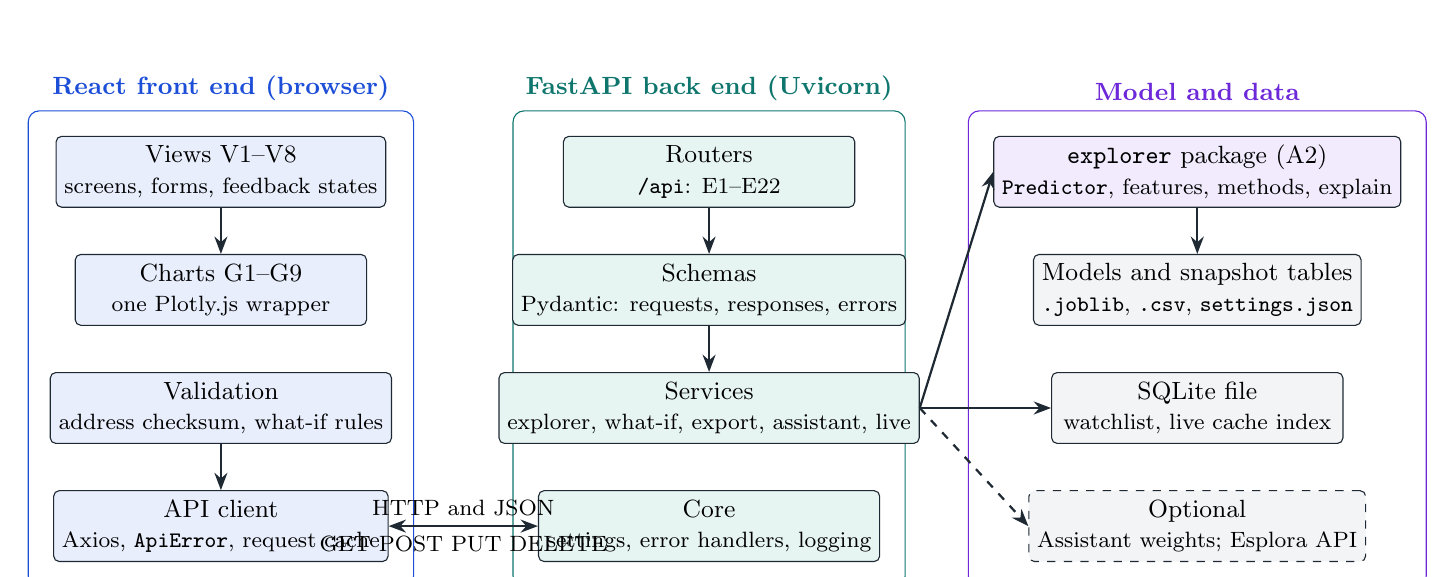
\begin{tikzpicture}[font=\small,
  box/.style={draw=ink, rounded corners=2pt, align=center, minimum width=3.7cm, minimum height=9mm, inner sep=3pt},
  fe/.style={box, fill=accentsoft},
  be/.style={box, fill=tealsoft},
  ml/.style={box, fill=violetsoft},
  st/.style={box, fill=greysoft},
  arr/.style={-{Stealth[length=2.2mm]}, thick, draw=ink},
  darr/.style={{Stealth[length=2.2mm]}-{Stealth[length=2.2mm]}, thick, draw=ink}]
  % front end
  \node[fe] (views)  at (0, 0)    {Views V1--V8\\ \footnotesize screens, forms, feedback states};
  \node[fe] (charts) at (0,-1.5)  {Charts G1--G9\\ \footnotesize one Plotly.js wrapper};
  \node[fe] (valid)  at (0,-3.0)  {Validation\\ \footnotesize address checksum, what-if rules};
  \node[fe] (client) at (0,-4.5)  {API client\\ \footnotesize Axios, \texttt{ApiError}, request cache};
  % back end
  \node[be] (routers)  at (6.2, 0)   {Routers\\ \footnotesize \texttt{/api}: E1--E22};
  \node[be] (schemas)  at (6.2,-1.5) {Schemas\\ \footnotesize Pydantic: requests, responses, errors};
  \node[be] (services) at (6.2,-3.0) {Services\\ \footnotesize explorer, what-if, export, assistant, live};
  \node[be] (core)     at (6.2,-4.5) {Core\\ \footnotesize settings, error handlers, logging};
  % model layer and stores
  \node[ml] (explorer) at (12.4, 0)   {\texttt{explorer} package (A2)\\ \footnotesize \texttt{Predictor}, features, methods, explain};
  \node[st] (files)    at (12.4,-1.5) {Models and snapshot tables\\ \footnotesize \texttt{.joblib}, \texttt{.csv}, \texttt{settings.json}};
  \node[st] (db)       at (12.4,-3.0) {SQLite file\\ \footnotesize watchlist, live cache index};
  \node[st, dashed] (opt) at (12.4,-4.5) {Optional\\ \footnotesize Assistant weights; Esplora API};
  % groups
  \begin{scope}[on background layer]
    \node[draw=accent, rounded corners=4pt, inner sep=9pt, fit=(views)(client), label={[font=\small\bfseries, text=accent]above:React front end (browser)}] (fegrp) {};
    \node[draw=teal, rounded corners=4pt, inner sep=9pt, fit=(routers)(core), label={[font=\small\bfseries, text=teal]above:FastAPI back end (Uvicorn)}] (begrp) {};
    \node[draw=violet, rounded corners=4pt, inner sep=9pt, fit=(explorer)(opt), label={[font=\small\bfseries, text=violet]above:Model and data}] (mlgrp) {};
  \end{scope}
  % arrows
  \draw[arr] (views) -- (charts);
  \draw[arr] (valid) -- (client);
  \draw[darr] (client.east) -- node[above, font=\footnotesize, align=center] {HTTP and JSON} node[below, font=\footnotesize, align=center] {GET POST PUT DELETE} (core.west |- client.east);
  \draw[arr] (routers) -- (schemas);
  \draw[arr] (schemas) -- (services);
  \draw[arr] (services.east) -- (explorer.west);
  \draw[arr] (explorer) -- (files);
  \draw[arr] (services.east) -- (db.west);
  \draw[arr, dashed] (services.east) -- (opt.west);
\end{tikzpicture}}
\caption{The layers. Solid arrows are calls made in the Must tier. Dashed parts are optional: the
application runs without them and says what is missing.}
\label{fig:arch}
\end{figure}

\textbf{Rules of the layering.}
\begin{itemize}
  \item A router only parses the request, calls one service function and returns its result. It
    never touches pandas or a model.
  \item A service never knows about HTTP. It raises the package's own exceptions
    (\code{Unsupported}, \code{InsufficientHistory}, \code{ValueError}); the core layer turns them
    into responses in one place.
  \item The \code{explorer} package is Assignment 2's code, copied unchanged. Every difference is
    in a service around it and is listed in Section~\ref{sec:mods}.
  \item A view never calls Axios. It calls a typed function of the API client and renders one of
    the request's four states: idle, loading, success, error.
  \item A view never draws with Plotly directly. It passes data to a chart component, which uses
    the one wrapper.
\end{itemize}

\subsection{One request, end to end}
\label{sec:walkthrough}

The what-if is the path the report and the video explain, because it crosses every layer.

\begin{enumerate}
  \item The user changes the amount in view V4. The form's rules run on the keystroke; an invalid
    value shows its message under the field and nothing is sent.
  \item 250 ms after the last change, the client cancels any request still in flight and sends
    \code{POST /api/addresses/{address}/what-if} with \code{amountBtc}, \code{direction} and
    \code{time}.
  \item FastAPI parses the body into a Pydantic model. A wrong type, an unknown field or a value
    out of range answers 400 with the \code{invalid} body and the failing field.
  \item The what-if service checks the address (404), converts the amount to whole satoshis and
    calls \code{Predictor.score_what_if}.
  \item \emph{Preprocessing.} The package builds the hypothetical row, giving it the median shape of
    the earlier transactions, appends it to the history strictly before its time, and computes the
    features F1 to F4 and their robust z-scores against the address's own comparison windows.
  \item \emph{Prediction.} The clipped z-scores and the direction go to each saved model; each
    returns a score, compared with that model's own threshold.
  \item \emph{Postprocessing.} The result becomes a transaction detail: values in BTC, the role of
    each feature, the comparison basis, every model's score and flag, the template explanation and
    the limitation line.
  \item The response model serialises it. The client resolves; the verdict card, the feature chart
    and the model table re-render, and the curve request (E9) follows.
\end{enumerate}

\subsection{Technology choices}
\label{sec:stack}

Versions are pinned on the first day and recorded in \code{environment.yml} and
\code{package-lock.json}; the report quotes them from those files.

{\small
\begin{longtable}{@{}L{2.5cm}L{3.3cm}L{8.2cm}@{}}
\toprule
\textbf{Part} & \textbf{Choice} & \textbf{Why, and what was not chosen} \\
\midrule
\endhead
Interface & React with TypeScript & Required by the brief; TypeScript carries the API contract into every screen (D-A3-2) \\
Build tool & Vite & Starts in seconds, proxies \code{/api}; create-react-app is deprecated \\
Charts & Plotly.js & D-A3-3. Not D3.js (every interaction by hand) or Chart.js (not on the High Distinction line) \\
Requests & Axios & D-A3-4. Cancellation and time limits for the live what-if \\
Routing & The prototype's hash router & Every view and state has a link; no server rewrite rules. Not React Router: 60 lines already do the job and are tested \\
Server state & The prototype's \code{useRequest} hook, extended with cancellation and polling & One small hook the team can explain. Not a query library: one more dependency for what three additions provide \\
Styling & The prototype's CSS with design tokens & Already responsive, themed and contrast-checked. Not a component kit: restyling every screen would gain nothing the rubric marks \\
Server & FastAPI on Uvicorn & Required by the brief; typed routes; generated OpenAPI documentation \\
Validation & Pydantic models & One definition gives parsing, validation, the response shape and the documentation \\
Model layer & Assignment 2's \code{explorer} package, pandas, scikit-learn, joblib & The brief: integrate the Assignment 2 model. Versions equal to Assignment 2's (D-A3-10) \\
Storage & CSV and joblib files; SQLite through the standard library & D-A3-8. Not an ORM: three small tables \\
Back-end tests & pytest with FastAPI's test client & Assignment 2's tool; requests run in-process, no server needed \\
Front-end tests & Vitest and Testing Library & The prototype's 66 tests keep running \\
Browser tests & Playwright (S-11) & Three widths, real browsers, screenshots for the report \\
\bottomrule
\end{longtable}
}

\subsection{Repository layout}
\label{sec:layout}

\begin{lstlisting}
COS30049A3/
  README.md                    set-up, run, configuration, tests, troubleshooting
  LICENSES.md  CHANGELOG.md
  backend/
    environment.yml  requirements.txt  requirements-assistant.txt
    app/
      main.py                  create_app(): lifespan, middleware, handlers, routers
      api/                     one router per resource
        system.py              E1 health, E2 config
        addresses.py           E3 list, E4 lookup, E5 timeline, E6 transactions, E20 delete
        transactions.py        E7 detail
        whatif.py              E8 single, E9 curve
        exports.py             E10
        methods.py             E11
        explanations.py        E12
        watchlist.py           E13-E15
        live.py                E16-E19
      schemas/                 Pydantic models: common, addresses, transactions, whatif, errors ...
      services/
        store.py               AddressStore: snapshot (and live) data behind one interface
        explorer_service.py    timeline, rows, detail; the per-address cache; method override
        whatif_service.py      single and batched what-if
        export_service.py      CSV and JSON
        assistant_service.py   lazy load, one answer at a time, cache
        watchlist_repo.py      SQLite
        live_service.py        jobs, Esplora fetch, progress events
      core/
        config.py              environment variables and settings.json -> web
        errors.py              exception classes and the handlers that build the error body
        validation.py          Bitcoin address and transaction-ID checks
        logging.py
    explorer/  lm/             Assignment 2's runtime modules, copied unchanged (A2_VENDOR.json)
    config/settings.json       Assignment 2's settings plus the "web" block
    models/                    the saved methods (about 30 MB)
    data/processed/esplora/    features.csv, transactions.csv, scores.csv, txgpt_scores.csv, manifest.json
    var/                       explorer.db, live cache, logs (git-ignored, created at start)
    tests/                     unit, API, parity, wording, performance smoke
    MODIFICATIONS.md           every change made for the web, with its test
  frontend/
    package.json  package-lock.json  vite.config.ts  tsconfig.json  index.html
    src/
      api/                     http.ts (Axios), endpoints.ts, types.ts, mock/ (tests only)
      views/                   V1-V8, one folder each
      charts/                  PlotlyChart.tsx (the wrapper) and G1-G9
      components/              buttons, badges, table, modal, toast, tabs, filter bar, fields ...
      hooks/                   useRequest, useDebounced, usePolling, useEventSource, usePreferences
      lib/                     address.ts, dates.ts, format.ts, router.ts, validation/
      styles/
    tests/                     unit, component, journeys
    e2e/                       Playwright (S-11)
  tools/
    vendor_a2.py               copies the runtime from the Assignment 2 repository, with hashes
    package.py                 builds the zip from a git tag, with SHA256SUMS.txt
    measure.py                 the performance table (S-12)
  docs/
    plan/  A3_delivery_plan.pdf   this plan
    brief/                     the brief (not in the zip)
    AI_USE_LOG.md  TEST_LOG.md  change-log.md  usability/
  report/                      the report's LaTeX (not in the zip)
\end{lstlisting}

\subsection{The address store}
\label{sec:store}

Services read addresses through one interface, so the snapshot and a fetched address look the same
to every endpoint.

\begin{itemize}
  \item \code{AddressStore.get(address)} returns the address's features, transactions and scores
    and its \code{source}: \code{snapshot} or \code{live}. It raises \code{Unsupported} when the
    address is in neither.
  \item The snapshot store wraps the \code{Predictor}'s three tables. It is filled once at start
    and never changes.
  \item The live store (S-09) adds an address after a lookup has fetched, cleaned, featured and
    scored its history. It is a folder of cached tables under \fp{var/live/}, named by the SHA-256
    of the address so that no user text reaches a file path.
  \item Every response that shows data carries \code{source} and its date, so the interface can
    label live data as live.
\end{itemize}

\subsection{Configuration}
\label{sec:config}

No value is typed into code. Numbers the web tier needs go into a new \code{web} block of
\fp{config/settings.json}; the front end reads them from E2, so the two tiers cannot disagree.

\begin{lstlisting}[style=json]
"web": {
  "whatIf":   { "minAmountBtc": 0.00000001, "maxAmountBtc": 21000000, "maxGapYears": 5,
                "curvePoints": 41, "curveMaxPoints": 61, "debounceMs": 250 },
  "lists":    { "pageSize": 50, "maxPageSize": 200 },
  "requests": { "timeoutMs": 10000, "assistantTimeoutMs": 90000, "healthPollSeconds": 15 },
  "charts":   { "webglMinPoints": 1000 },
  "watchlist":{ "maxEntries": 200, "maxLabelChars": 40, "maxNoteChars": 500 },
  "live":     { "defaultMaxTx": 500, "maxTxLimit": 1000, "lookupsPerHour": 6, "cacheDays": 7 },
  "replay":   { "speeds": [1, 5, 20] },
  "limits":   { "maxBodyBytes": 10240, "maxAddressChars": 100 }
}
\end{lstlisting}

Values here are starting points\est{}; a change is logged in \fp{CHANGELOG.md} as in Assignment 2.
Environment variables only choose what a machine may do:

\begin{center}
\small
\begin{tabularx}{\textwidth}{@{}L{4.6cm}L{4.2cm}Y@{}}
\toprule
\textbf{Variable} & \textbf{Default} & \textbf{Meaning} \\
\midrule
\code{EXPLORER_CORS_ORIGINS} & \code{http://localhost:5173}, \code{http://127.0.0.1:5173} & Origins allowed to call the API directly \\
\code{EXPLORER_LIVE_LOOKUP} & \code{off} & Turns S-09 on; needs CR-08 \\
\code{EXPLORER_ASSISTANT} & \code{auto} & \code{auto}: on when the weights are present; \code{off}: template only \\
\code{EXPLORER_LOG_LEVEL} & \code{INFO} & Log detail \\
\code{VITE_API_BASE} (front end) & empty & Empty: same origin through Vite's proxy; else the back end's address \\
\code{VITE_API_MODE} (front end) & \code{http} & \code{mock} runs the screens on the in-browser mock, for tests \\
\bottomrule
\end{tabularx}
\end{center}

\subsection{Ways to run it}
\label{sec:runmodes}

\begin{center}
\small
\begin{tabularx}{\textwidth}{@{}L{2.8cm}Y L{1.6cm}@{}}
\toprule
\textbf{Mode} & \textbf{How} & \textbf{Tier} \\
\midrule
Development and marking & Terminal 1: \code{uvicorn app.main:app --port 8000} in \fp{backend/}. Terminal 2: \code{npm run dev} in \fp{frontend/}, then open \code{http://localhost:5173}. The API's documentation is at \code{http://localhost:8000/docs} & \must \\
Tests & \code{python -m pytest -q} in \fp{backend/}; \code{npm test} in \fp{frontend/}. Neither needs the other tier running & \must \\
One command & \code{npm run build}, then Uvicorn serves \fp{frontend/dist} at \code{/}; or \code{docker compose up} & \could{} (C-05) \\
\bottomrule
\end{tabularx}
\end{center}

\begin{done}
A fresh clone starts both tiers with the README's commands in under 15 minutes including installs,
the back end reports ready within 10 seconds of starting\est{} (5.6 s measured for import and load
on the Mac), and the browser console and both terminals show no error or warning.
\end{done}

\section{The API}
\label{sec:api}

This is the contract both tiers build against. FastAPI generates the same information as an OpenAPI
schema, served at \code{/docs}, \code{/redoc} and \code{/openapi.json}; the report's API section is
written from that schema so the two cannot differ.

\subsection{Conventions}
\label{sec:apiconventions}

\begin{itemize}
  \item \textbf{Base and format.} Every path starts with \code{/api}. Bodies are JSON in UTF-8,
    except the CSV export (E10) and the progress stream (E18). Names are camelCase, as in
    Assignment 1's contract and \code{predict.py}.
  \item \textbf{Resources.} Paths name things (addresses, transactions, methods, watchlist entries,
    lookups), and the HTTP method says what happens: GET reads and changes nothing; POST computes
    from a body or starts a job; PUT creates or replaces the named entry and can be repeated safely;
    DELETE removes it. Assignment 1's \code{POST /api/lookup} keeps its name because it was promised.
  \item \textbf{Times and amounts.} Times are ISO 8601 in UTC, such as \code{2026-10-20T12:00:00Z}.
    Days are \code{YYYY-MM-DD} in UTC. Amounts in responses are whole satoshis (\code{netSats});
    feature values are in the units people read (BTC, count, hours, ratio). The what-if request
    takes \code{amountBtc}, with up to eight decimal places.
  \item \textbf{Lists.} \code{page} starts at 1; \code{pageSize} defaults to 50 and stops at 200.
    A list answers with its rows, \code{page}, \code{pageSize} and \code{total}. No rows is a 200
    with an empty list, never an error.
  \item \textbf{Errors.} One body for every failure (Section~\ref{sec:errorbody}).
  \item \textbf{Headers.} Every response carries \code{X-Request-ID}. Snapshot data carries an
    \code{ETag} and \code{Cache-Control: no-cache}, so a repeat request costs a 304. Responses over
    1 kB are compressed with gzip.
  \item \textbf{The deciding method.} E3, E5, E6, E7 and E10 accept \code{method=} (S-01). Without
    it they use \code{explorerMethod}, the baseline.
\end{itemize}

\subsection{Every endpoint}
\label{sec:endpoints}

{\small
\begin{longtable}{@{}L{0.7cm}L{1.3cm}L{6.6cm}L{4.0cm}L{1.7cm}@{}}
\toprule
\textbf{No.} & \textbf{Method} & \textbf{Path} & \textbf{Returns} & \textbf{Tier} \\
\midrule
\endhead
E1 & GET & \code{/api/health} & Ready or starting; what is loaded & \must \\
E2 & GET & \code{/api/config} & Snapshot, limits, thresholds, feature names, capabilities & \must \\
E3 & GET & \code{/api/addresses} & The addresses that can be opened, with counts & \must{} (A1) \\
E4 & POST & \code{/api/lookup} & Whether a typed address is supported & \must{} (A1) \\
E5 & GET & \code{/api/addresses/{address}/timeline} & Per-day counts, totals, range, history status & \must{} (A1) \\
E6 & GET & \code{/api/addresses/{address}/transactions} & A filtered, sorted page of transaction rows & \must{} (A1, extended) \\
E7 & GET & \code{/api/transactions/{txid}?address=} & One transaction: facts, features, reason, every model's verdict & \must{} (A1) \\
E8 & POST & \code{/api/addresses/{address}/what-if} & A hypothetical transaction's verdict from every model & \must \\
E9 & POST & \code{/api/addresses/{address}/what-if/curve} & Scores over a range of amounts & \must \\
E10 & GET & \code{/api/addresses/{address}/export} & The scored transactions as a CSV or JSON file & \must \\
E11 & GET & \code{/api/methods} & The nine methods, their thresholds and test results & \must \\
E12 & POST & \code{/api/explanations} & The Assistant's guarded explanation, or the template & \should{} S-05 \\
E13 & GET & \code{/api/watchlist} & The watched addresses with labels and notes & \should{} S-04 \\
E14 & PUT & \code{/api/watchlist/{address}} & Adds or replaces an entry & \should{} S-04 \\
E15 & DELETE & \code{/api/watchlist/{address}} & Removes an entry & \should{} S-04 \\
E16 & POST & \code{/api/live/lookups} & Starts a live lookup; answers 202 with its identifier & \should{} S-09 \\
E17 & GET & \code{/api/live/lookups/{id}} & The lookup's status and progress & \should{} S-09 \\
E18 & GET & \code{/api/live/lookups/{id}/events} & The same as a stream of events & \should{} S-09 \\
E19 & DELETE & \code{/api/live/lookups/{id}} & Cancels the lookup & \should{} S-09 \\
E20 & DELETE & \code{/api/addresses/{address}} & Forgets a fetched address & \should{} S-09 \\
E21 & GET & \code{/api/addresses/{address}/surprisal} & TxGPT's surprisal per field & \could{} C-01 \\
E22 & GET & \code{/api/addresses/{address}/profile} & The address's activity profile & \could{} C-02 \\
\bottomrule
\end{longtable}
}

The Must tier uses GET and POST across eleven endpoints, which meets the brief's ``at least two
HTTP methods''. S-04 adds PUT and DELETE on a resource where they mean what REST says they mean.

\subsection{The error body and the status codes}
\label{sec:errorbody}

\begin{lstlisting}[style=json]
{
  "status": "invalid",
  "message": "The amount must be greater than zero.",
  "hint": "Enter an amount in BTC, such as 0.05.",
  "fields": [ { "name": "amountBtc", "message": "Must be greater than 0." } ],
  "requestId": "0f3c9a1e7b2d"
}
\end{lstlisting}

\code{status} is for the code, \code{message} and \code{hint} are plain words that are safe to
show, \code{fields} names the form fields at fault, and \code{requestId} matches the server's log
line. The first three are Assignment 1's bodies unchanged; \code{fields} and \code{requestId} are
additions. Some statuses add their own keys, as Assignment 1 planned: \code{examples} with
\code{unsupported}, and \code{transaction}, \code{history} and \code{firstScoredDate} with
\code{insufficient_history}.

{\small
\begin{longtable}{@{}L{0.9cm}L{3.6cm}L{5.2cm}L{4.2cm}@{}}
\toprule
\textbf{Code} & \textbf{\code{status}} & \textbf{When} & \textbf{Raised by} \\
\midrule
\endhead
200 & -- & Success with a body & \\
201 & -- & A watchlist entry was created & E14 \\
202 & -- & A live lookup was accepted and is running & E16 \\
204 & -- & Removed; no body & E15, E19, E20 \\
304 & -- & The cached copy is still right & snapshot GETs \\
400 & \code{invalid} & A malformed address, date, transaction ID, number, choice or body; an unknown field; \code{from} after \code{to} & Pydantic validation, the address checker, \code{ValueError} \\
403 & \code{disabled} & Live lookup is switched off on this server & E16 to E20 \\
404 & \code{unsupported} & A valid address that is not in the snapshot or the live cache; carries three examples & \code{Unsupported} \\
404 & \code{not_found} & An unknown transaction for that address, watchlist entry, lookup or path & \code{Unsupported}, the repositories \\
409 & \code{conflict} & The watchlist is full; a lookup for that address is already running; a snapshot address cannot be forgotten & E14, E16, E20 \\
413 & \code{too_large} & A body over the size limit & middleware \\
415 & \code{invalid} & A body that is not JSON & FastAPI \\
422 & \code{insufficient_history} & Too little earlier history to score: the address, the transaction, or the what-if's time & \code{InsufficientHistory} \\
429 & \code{rate_limited} & Too many live lookups, or the Assistant is busy; carries \code{Retry-After} & E12, E16 \\
500 & \code{server_error} & Anything unexpected. A fixed message and the request identifier; the trace goes to the log only & the catch-all handler \\
502 & \code{upstream_error} & Esplora answered with an error & E16 to E18 \\
503 & \code{unavailable} & The models are still loading, or a file is missing & E1; \code{FileNotFoundError} \\
504 & \code{upstream_timeout} & Esplora did not answer in time & E16 to E18 \\
\bottomrule
\end{longtable}
}

\begin{caution}
FastAPI's own validation error is a 422 with a \code{detail} list. The handler for
\code{RequestValidationError} is replaced so that it answers 400 with the body above (D-A3-5). A
test posts a wrong type to every POST and PUT endpoint and checks for 400 and \code{fields}.
\end{caution}

\subsection{Endpoints in detail}

Shapes marked A1 are those of \fp{frontend/src/api/types.ts} in the prototype. Full example bodies
are in Appendix~\ref{app:json}.

\subsubsection*{E1 \quad GET /api/health}
Answers 200 with \code{status: "ok"}, the application version, \code{snapshotDate},
\code{addressCount}, \code{methodCount}, \code{assistant} (\code{ready}, \code{not_installed},
\code{loading} or \code{off}), \code{liveLookup} (true or false) and \code{uptimeSeconds}. While the
models load it answers 503 with \code{status: "unavailable"}. Never cached. The front end polls it
for the service-status indicator, and the README uses it as the first check.

\subsubsection*{E2 \quad GET /api/config}
Everything the front end would otherwise hard-code: \code{snapshot} (date, source, link, address
count, method), \code{limitationLine}, \code{features} (identifier, name, description and unit of F1
to F4), \code{history} (the minimum of 10 transactions over 14 days), \code{thresholds} (the flag
line 5.0 and the contributing line 2.0), \code{defaultMethod}, the \code{web} block of
Section~\ref{sec:config}, \code{whatIf.defaultTime} (noon UTC on the snapshot date) and
\code{capabilities} (\code{assistant}, \code{liveLookup}).

\subsubsection*{E3 \quad GET /api/addresses}
A1's \code{AddressesResponse}: \code{snapshot} and \code{addresses}. Each address has
\code{address}, \code{firstSeen}, \code{lastSeen}, \code{txCount}, \code{scoredCount},
\code{flaggedCount} and \code{history} (\code{sufficient} or \code{insufficient}). Added:
\code{kind} (the address type, such as P2PKH), \code{source} (\code{snapshot} or \code{live}) and,
with S-04, \code{watch} (label and note, or null). Main addresses come first, busiest first; the
short-history ones last, as in the terminal Explorer.

\subsubsection*{E4 \quad POST /api/lookup}
Body: \code{address}. 200 with \code{status: "supported"}, the normalised \code{address} and its
\code{summary}. 400 \code{invalid} with the checker's specific message, such as ``This address fails
its checksum, so it probably contains a typo.'' 404 \code{unsupported} with the coverage sentence
and three \code{examples}; with S-09 it adds \code{canLookupLive}.

\subsubsection*{E5 \quad GET /api/addresses/\{address\}/timeline}
A1's \code{TimelineResponse}: \code{address}, \code{snapshot}, \code{range} (first and last
transaction time), \code{days} (only days with transactions, oldest first, each with
\code{txCount} and \code{flaggedCount}), \code{totals} (\code{txCount}, \code{scoredCount},
\code{flaggedCount}, \code{flaggedDays}) and \code{history} (\code{status}, \code{txCount},
\code{spanDays}, \code{required}, \code{firstScoredDate}). A short-history address answers 200 with
\code{history.status: "insufficient"} and \code{scoredCount: 0}, so the screen can list its
transactions unscored. Errors: 400, 404 \code{unsupported}.

\subsubsection*{E6 \quad GET /api/addresses/\{address\}/transactions}
\begin{center}
\small
\begin{tabularx}{\textwidth}{@{}L{2.4cm}L{4.3cm}Y@{}}
\toprule
\textbf{Query} & \textbf{Values} & \textbf{Meaning} \\
\midrule
\code{date} & \code{YYYY-MM-DD} & One UTC day (A1's parameter) \\
\code{from}, \code{to} & \code{YYYY-MM-DD} & An inclusive range of days; not with \code{date} \\
\code{status} & \code{flagged}, \code{not-flagged}, \code{not-scored}; may repeat & Keep these statuses \\
\code{direction} & \code{in}, \code{out}, \code{none}; may repeat & Keep these directions \\
\code{sort} & \code{time}, \code{amount}, \code{score}; a leading minus reverses & Default \code{time} \\
\code{page}, \code{pageSize} & whole numbers & Default 1 and 50; at most 200 a page \\
\code{method} & a method identifier & Whose flags and scores to show (S-01) \\
\bottomrule
\end{tabularx}
\end{center}
Answers \code{address}, \code{date} (or null), \code{transactions}, \code{page}, \code{pageSize}
and \code{total}. A row is A1's \code{TransactionRow} (\code{txid}, \code{time}, \code{direction},
\code{netSats}, \code{status}) plus \code{score} (the deciding method's, or null),
\code{mainReason} (the template's strongest reason, such as ``Longer gap than usual''),
\code{mainZ} and \code{flaggedBy} (how many methods flag it). A day or a filter that matches
nothing is a 200 with an empty list. Errors: 400 for a malformed or contradictory query, 404
\code{unsupported}.

The scatter chart asks for up to 200 rows a page and joins the pages; the largest snapshot address
needs four requests.

\subsubsection*{E7 \quad GET /api/transactions/\{txid\}?address=}
A1's \code{TransactionDetail}: the facts (\code{txid}, \code{address}, \code{time},
\code{blockHeight}, \code{direction}, \code{receivedSats}, \code{sentSats}, \code{netSats},
\code{sourceUrl}), \code{scored}, \code{flagged}, \code{score}, \code{method}, \code{features}
(for each of F1 to F4: \code{value}, \code{usual}, \code{z} and \code{role}), \code{comparison}
(what each feature was compared with: how many earlier transactions, from when to when) and
\code{limitation}. Added, all already returned by \code{predict.py}: \code{explanation} (the
template text), \code{scores} and \code{flags} for every method, and \code{source}. Errors: 400
(a transaction ID that is not 64 hexadecimal characters, or no \code{address}); 404
\code{unsupported} (the address); 404 \code{not_found} (the transaction is not that address's);
422 \code{insufficient_history} with the transaction's facts when it could not be scored.

\subsubsection*{E8 \quad POST /api/addresses/\{address\}/what-if}
\label{sec:e8}
\begin{center}
\small
\begin{tabularx}{\textwidth}{@{}L{2.2cm}L{3.1cm}Y@{}}
\toprule
\textbf{Field} & \textbf{Type} & \textbf{Rule} \\
\midrule
\code{amountBtc} & number or decimal string & Greater than 0; at least 0.00000001; at most 21,000,000; at most 8 decimal places \\
\code{direction} & \code{"in"} or \code{"out"} & Required \\
\code{time} & ISO 8601 with a zone & Not before the address's first transaction (else 422); not more than \code{maxGapYears} after its last (else 400) \\
\bottomrule
\end{tabularx}
\end{center}
200: a transaction detail as E7 with \code{txid: "what-if"}, \code{sourceUrl: null}, the template
\code{explanation}, \code{scores} and \code{flags} from the eight methods that can score new input,
\code{notAvailable: ["txgpt_method"]} and a \code{note} that the transaction is hypothetical.
Nothing is stored. Errors: 400 \code{invalid} with \code{fields}; 404 \code{unsupported}; 422
\code{insufficient_history} when fewer than 10 transactions or 14 days of history precede the
chosen time, with the counts and the first date that can be scored.

\subsubsection*{E9 \quad POST /api/addresses/\{address\}/what-if/curve}
Body: \code{direction} and \code{time} as E8, then either \code{amountsBtc} (a list of up to 61
amounts) or \code{minBtc}, \code{maxBtc} and \code{points}. With neither, the server spaces 41
amounts evenly on a log scale from one hundredth of the address's usual amount in that direction to
a thousand times it. 200: \code{amountsBtc}, \code{usualBtc}, \code{decidingMethod}, and for each
method its \code{threshold}, \code{scores} and \code{flags}, one per amount. One feature build
scores every amount (Section~\ref{sec:whatif}). Errors as E8.

\subsubsection*{E10 \quad GET /api/addresses/\{address\}/export}
Query: \code{format} (\code{csv}, the default, or \code{json}) and E6's filters. Answers a file
with \code{Content-Disposition: attachment}, named from the first eight characters of the address
and the snapshot date. CSV columns: address, transaction ID, time (UTC), direction, received, sent
and net amount in BTC, scored, flagged, deciding method, score, each feature's value, usual value
and z, the main reason, the methods that flag it, the source link, the snapshot date and, on
flagged rows, the limitation line. A cell that starts with \code{=}, \code{+}, \code{-} or
\code{@} is written with a leading apostrophe, so a spreadsheet does not run it as a formula.

\subsubsection*{E11 \quad GET /api/methods}
\code{defaultMethod} and \code{methods}. Each has \code{id}, \code{name}, \code{family} (statistics,
outlier detection, clustering, regression, combination, language model), a one-sentence
\code{description}, its \code{threshold}, \code{scoresNewInput} and \code{evaluation}: mean recall
on planted transactions with its 95\% interval, recall per pattern (spike, burst, dormant) and the
flag rate on real transactions. The evaluation numbers are read from copies of Assignment 2's
\fp{eval_significance.csv} and \fp{eval_selection.csv}; none is typed.

\subsubsection*{E12 \quad POST /api/explanations \quad (S-05)}
Body: \code{address} and either \code{txid} or a \code{whatIf} object as E8. 200: \code{txid},
\code{flagged}, \code{explanation}, \code{source} (\code{text150m} or \code{template}),
\code{cached}, \code{attempts} (each writer tried and the guardrail checks it failed),
\code{skippedWriters} (a writer this machine cannot run, and why), \code{limitation} and
\code{seconds}. A rejected answer is never returned. Errors: 400, 404, 422; 429 while another
answer is being written.

\subsubsection*{E13 to E15 \quad the watchlist \quad (S-04)}
\code{GET /api/watchlist} lists entries (\code{address}, \code{label}, \code{note}, \code{addedAt},
\code{updatedAt} and the address's summary). \code{PUT /api/watchlist/{address}} with
\code{label} (40 characters at most) and \code{note} (500 at most) answers 201 for a new entry and
200 for a replaced one; 404 \code{unsupported} for an address that cannot be opened; 409 when the
list holds 200 entries. \code{DELETE} answers 204, or 404 \code{not_found}.

\subsubsection*{E16 to E20 \quad live lookup \quad (S-09, CR-08)}
\code{POST /api/live/lookups} with \code{address} and optional \code{maxTx} (50 to 1,000; default
500) answers 202 with the lookup's \code{id}, its \code{status} and links to E17 and E18, and a
\code{Location} header. A fresh cached result answers 200 at once. \code{GET} E17 returns
\code{status} (\code{queued}, \code{fetching}, \code{scoring}, \code{done}, \code{failed},
\code{cancelled}), \code{progress} (pages and transactions fetched, the cap) and, on failure, an
error body. E18 sends the same as server-sent events named \code{progress}, \code{status},
\code{done} and \code{failed}, with a comment line every 15 seconds to keep the connection open.
E19 cancels. Once done, the address answers E5 to E10 like a snapshot address, with
\code{source: "live"} and the time it was fetched; E20 forgets it.

\subsubsection*{E21, E22 \quad (Could)}
E21 returns, for a snapshot address, each transaction's surprisal in total and for the six token
fields (gap, direction, amount, inputs, outputs, fee). E22 returns the address's profile from
Assignment 2's profile model: its label, its eight address-level features and the profile's medians.

\subsection{What the report documents}

The brief asks for at least four endpoints. The report gives the table of
Section~\ref{sec:endpoints}, the error body, and four endpoints in full with a request and a real
response each: E4 (a POST with all three outcomes), E5, E7 and E8. The complete reference, exported
from \code{/openapi.json}, goes in the appendix, which does not count towards the eight pages.

\begin{done}
Every endpoint in a finished tier has a response model, appears in \code{/docs} with a summary and
an example, and has one test for its success and one for each error in its row. \code{GET} E3 to E7
return exactly what \code{Predictor} returns for all 28 addresses (the parity test of
Section~\ref{sec:tests}).
\end{done}

\section{AI model integration}
\label{sec:model}

The brief's wording for full points is ``seamlessly integrated, provides real-time predictions,
and handles various input types''. The application serves nine scoring methods and one language
model from Assignment 2, takes four kinds of input (an address, a transaction of that address, a
hypothetical transaction, and a choice of method), and answers each from memory or in well under a
second.

\subsection{The methods the application serves}
\label{sec:methods}

Names, thresholds and sizes are read from the Assignment 2 repository at commit \code{aa56a26}. A
transaction is flagged by a method when it can be scored and its score reaches that method's
threshold.

{\small
\begin{longtable}{@{}L{3.4cm}L{2.0cm}L{4.2cm}L{1.3cm}L{2.7cm}@{}}
\toprule
\textbf{Method} & \textbf{Family} & \textbf{What its score measures} & \textbf{Flag at} & \textbf{File} \\
\midrule
\endhead
Robust z baseline (A1) \newline \code{baseline} & Statistics & The largest $|z|$ of F1 to F4 against the address's own median and spread. Nothing is trained & 5.0 & \fp{baseline.json} \newline 1 kB \\
Isolation Forest \newline \code{isolation_forest} & Outlier detection & How easily random trees isolate the transaction & 0.589 & \fp{isolation_forest.joblib} \newline 2.8 MB \\
Local Outlier Factor \newline \code{lof} & Outlier detection & Local density against the nearest neighbours & 1.855 & \fp{stage/C3_lof.joblib} \newline 3.3 MB \\
K-Means distance \newline \code{kmeans} & Clustering & Distance to the nearest cluster centre & 9.978 & \fp{stage/C4_kmeans.joblib} \newline 2 kB \\
DBSCAN noise \newline \code{dbscan} & Clustering & Distance to the nearest dense core & 2.821 & \fp{stage/C5_dbscan.joblib} \newline 0.3 MB \\
Regression residual \newline \code{regression} & Regression & The miss between the predicted and actual size and gap & 3.5 & \fp{regression.joblib} \newline 1.7 MB \\
Regression expected range \newline \code{regression_interval} & Regression & Distance outside the conformal expected range & 0.0 & \fp{regression_interval.joblib} \newline 0.5 MB \\
Score fusion \newline \code{fusion} & Combination & Regression and Isolation Forest together, at one flag budget & 1.0 & \fp{fusion.joblib} \newline 5.0 MB \\
TxGPT surprisal \newline \code{txgpt_method} & Language model & How surprising the transaction's tokens are to TxGPT, trained from scratch on the crawl & 12.203 & \fp{txgpt_method.joblib} \newline 17.5 MB \\
\bottomrule
\end{longtable}
}

The nine files total about 31 MB and go in the zip. TxGPT's scores for the snapshot were computed
in advance and are stored with its method, so it shows a verdict for every snapshot transaction but
not for a what-if; the interface says ``not available for a hypothetical transaction'' in its row.
The tenth model, the 152M Explorer Assistant, writes explanations and scores nothing
(Section~\ref{sec:assistant}).

\textbf{The method selector (S-01).} Every snapshot transaction already has a score and a flag
from all nine methods in \fp{scores.csv}. Choosing a method changes which column decides
\code{flagged}, \code{score}, the daily flagged counts and the chart colours. The explanation then
opens with ``Flagged by Isolation Forest.'' and lists what stands out in F1 to F4, or the two largest
differences when nothing does, exactly as Assignment 2's template does for any method. The service
makes this view with \code{dataclasses.replace(predictor, selected=method)}, which shares the loaded
tables. The selector always shows which method is active and offers ``Back to the default''.

\subsection{From input to output}
\label{sec:prepost}

The report must describe preprocessing and postprocessing. These are the stages and where each
lives.

\begin{center}
\small
\begin{tabularx}{\textwidth}{@{}L{2.6cm}Y L{4.1cm}@{}}
\toprule
\textbf{Stage} & \textbf{What happens} & \textbf{Code} \\
\midrule
Validate & Address checksum and network; transaction ID; amount, direction and time ranges & \fp{app/core/validation.py}, the schemas \\
Look up & The address's rows, from the snapshot or the live cache & \fp{services/store.py} \\
Preprocess & Amount to satoshis; the hypothetical row with the history's median shape; features F1 to F4 from strictly earlier transactions; robust z-scores against two comparison windows; z clipped to $\pm 20$; direction as two indicator columns & \fp{explorer.features}, \fp{explorer.methods.model_inputs} \\
Predict & Each saved method's \code{score}; compared with its threshold & \fp{explorer.methods.flags}, the method classes \\
Postprocess & Units people read (BTC, hours, counts); each feature's role (flag, contributing, within usual); the comparison basis; the template explanation; the limitation line on flags; NaN to null & \fp{Predictor.detail}, \fp{explorer.explain} \\
Check & No banned word in any text; the response matches its model & \code{check_outputs}, the response model \\
\bottomrule
\end{tabularx}
\end{center}

Snapshot transactions were preprocessed and scored when Assignment 2 froze its results, so a GET
only reads and postprocesses. The time-safety rule holds everywhere: a feature uses only
transactions confirmed strictly earlier at the same address, and transactions with the same time are
never each other's history.

\subsection{The what-if, single and batched}
\label{sec:whatif}

\textbf{Single (E8).} \code{Predictor.score_what_if} as it is: 0.40 s measured.

\textbf{Batched (E9).} The curve needs the same transaction at many amounts. Called one by one,
41 amounts would take about 16 s\est{}. Because same-time transactions are never each other's
history, all the hypothetical rows can share one time and go through one feature build: each sees
only the real, earlier history.

\begin{lstlisting}[style=py]
rows = [hypothetical(address, amount, direction, t, txid=f"what-if-{i:03d}")
        for i, amount in enumerate(amounts)]            # same time t, distinct ids
frame = build_features(pd.concat([earlier, pd.DataFrame(rows)]), FeatureConfig.refined())
new = frame[frame["txid"].str.startswith("what-if")].assign(period="eval")
scores = {name: method.score(new) for name, method in usable.items()}
\end{lstlisting}

Measured on the running example with seven amounts from 0.0001 to 10 BTC: 0.16 s for the batch
against 1.88 s for seven single calls, and the scores of all eight methods equal to six decimal
places. The default curve of 41 amounts, from a hundredth of the usual amount to a thousand times
it, took 0.18 s for all eight methods. On it the baseline's score falls from 5.94 at the smallest
amount to 0.45 at the usual one and rises to 9.00 at the largest: an amount far below the usual
stands out as well as one far above. The flag line of 5.0 is crossed at about 0.023 BTC on the way
up and at about 0.00001 BTC on the way down.

\begin{done}
A parity test scores 41 amounts both ways on three addresses and both directions and requires equal
scores and flags for every method. E9 answers in under 1.5 s on the PC and the Mac.
\end{done}

\subsection{Copying Assignment 2's runtime}
\label{sec:vendoring}

\code{tools/vendor_a2.py --from ../COS30049A2 --commit <sha>} does the copy, so it can be repeated
and checked.

\begin{enumerate}
  \item It checks out nothing: it reads files from the given commit with \code{git show}, so
    uncommitted work cannot leak in.
  \item It finds the modules to copy by loading the entry points in a clean interpreter
    (\code{Predictor.load()}, one \code{score_address}, one \code{score_what_if}) and listing every
    \code{explorer} and \code{lm} module that was imported. On 10 November that list was 23
    \code{explorer} modules and \code{lm.tx_tokens}: \code{amounts}, \code{assistant},
    \code{baseline}, \code{classify}, \code{clustering}, \code{esplora}, \code{explain},
    \code{external}, \code{features}, \code{fusion}, \code{inject}, \code{labelled},
    \code{methods}, \code{outliers}, \code{predict}, \code{regression}, \code{scores},
    \code{settings}, \code{snapshot}, \code{split}, \code{stage_search}, \code{stages} and
    \code{txgpt}. S-05 adds the Assistant's modules of \code{lm} the same way; S-09 adds
    \code{transactions} and the frozen-model adapter.
  \item It copies the nine method files, \fp{selection.json}, \fp{profiles.joblib}, the four
    snapshot tables and the manifest, \fp{config/settings.json}, and the two evaluation tables E11
    reads.
  \item It writes \fp{backend/A2_VENDOR.json}: the source commit, the date, and a SHA-256 for every
    copied file.
\end{enumerate}

\begin{caution}
The package keeps the name \code{explorer} and its module names. The saved models are pickles that
record each class by its module path; a renamed module would make them fail to load. No file under
\fp{backend/explorer/} or \fp{backend/lm/} is edited by hand. A test recomputes every hash against
\fp{A2_VENDOR.json}.
\end{caution}

\subsection{Modifications for the web}
\label{sec:mods}

The brief asks the report to list ``any modifications for web deployment''. Every one is in a
service around the copied package, is written up in \fp{backend/MODIFICATIONS.md}, and has a test.

{\small
\begin{longtable}{@{}L{1.2cm}L{5.4cm}L{4.4cm}L{3.0cm}@{}}
\toprule
\textbf{No.} & \textbf{Modification} & \textbf{Why} & \textbf{Test} \\
\midrule
\endhead
Mod-1 & The models and tables load once, in the application's lifespan, and are shared read-only & A load takes 0.9 s; a request must not pay it & Start-up test; health reports the counts \\
Mod-2 & A per-address cache of the scored result, filled lazily and warmed for all 28 addresses in the background after start & Repeat views answer from memory & Second request faster than the first; equal bodies \\
Mod-3 & \code{score_address}'s single result is split into timeline, a page of rows and one detail & It is up to 2 MB; a view needs a few kB & Parity: the pieces rebuild the whole \\
Mod-4 & A timeline for addresses with too little history, built from the feature table & \code{score_address} raises for them, but A1's screen lists their transactions unscored & The three short-history addresses answer 200 \\
Mod-5 & The batched what-if (Section~\ref{sec:whatif}) & 41 amounts in one feature build & Parity with single calls \\
Mod-6 & A what-if that cannot be scored answers 422 with the history counts & A1's meaning of 422; the form can say which date would work & Early-time what-if \\
Mod-7 & The deciding method can be chosen per request & S-01 & Flags equal \fp{scores.csv} for each method \\
Mod-8 & Exceptions become HTTP errors in one place: \code{Unsupported} 404, \code{InsufficientHistory} 422, \code{ValueError} 400 & One error body & One test per mapping \\
Mod-9 & The Assistant loads on first use behind a lock, writes one answer at a time off the event loop, and caches answers by a hash of the facts & An answer takes about 10 s of CPU; two at once would double it & Second request is cached; a busy request gets 429 \\
Mod-10 & Start-up checks: library versions against the pins, every model file against its hash, a named count of worker threads & A clear message, not a flood of warnings & Wrong version stops with the message \\
Mod-11 & Frozen models applied to a fetched address, with the regression's residual scales set from that address's own earlier 70\% & S-09; the route Assignment 2 used for its held-out snapshot & Parity with Assignment 2's DS10 scores on one address \\
\bottomrule
\end{longtable}
}

\subsection{The Explorer Assistant (S-05)}
\label{sec:assistant}

\begin{itemize}
  \item \textbf{What the user sees.} Every explanation starts as the template, labelled ``Template:
    fixed sentences filled in from the numbers''. A button, ``Ask the Assistant to write this'',
    appears when \code{capabilities.assistant} is true. While it writes, the panel shows a progress
    line (``Writing; this takes about 10 seconds on this computer'') and a ``Keep the template''
    button that cancels. The answer replaces the template with the label ``Written by the Explorer
    Assistant, a language model the team trained; checked by code before being shown''.
  \item \textbf{The guardrail.} Six checks from \code{explorer.assistant.check}: every number comes
    from the facts, the limitation line is present on a flag, no banned word, the comparison words
    point the right way, the verdict matches, and the answer is not empty. A failed answer is
    discarded; the template stays, with a line naming the failed checks.
  \item \textbf{Not installed.} Without the weights the button is replaced by a note: ``The
    Assistant's model file (610 MB) is not installed; the README says how to add it. Explanations
    use the template.'' Nothing else changes.
  \item \textbf{Speed.} Decoding is greedy, so the same facts always give the same answer; answers
    are cached by a SHA-256 of the facts. \code{tools/precompute_assistant.py} writes the guarded
    answers for the snapshot's flagged transactions under the baseline to a JSON file that ships in
    the zip, so a marker without the weights still reads Assistant-written explanations there. A
    what-if or a fetched address needs the weights.
  \item \textbf{Limits.} One answer at a time; a second request waits its turn through a 429 and an
    automatic retry. The request's time limit is 90 seconds, the first load included.
\end{itemize}

\subsection{The live lookup (S-09, needs CR-08)}
\label{sec:live}

\begin{enumerate}
  \item The user types a valid address that is not in the snapshot. The unsupported state explains
    the coverage as before and, when live lookup is on, adds ``Fetch this address's public history''.
  \item \code{POST /api/live/lookups} starts a background job and answers 202. The job pages
    through Esplora's confirmed history, newest first, 25 transactions a page, with Assignment 2's
    client: paced requests, back-off, and a switch to the second host when the first limits the rate.
  \item Progress events drive a dialog: pages and transactions so far against the cap, and a
    Cancel button. The fetch stops at \code{maxTx} (500 by default), so it needs at most 20 pages.
  \item The history is cleaned (\code{build_transactions}), featured (\code{build_features}),
    split at 70\% (\code{assign_periods}) and scored by the frozen methods through Assignment 2's
    adapter. TxGPT is skipped unless PyTorch is installed.
  \item The result goes into the live store; the overview opens with a ``Live data, fetched
    10 Nov 2026 14:02 UTC, the most recent 500 transactions'' banner in place of the snapshot date.
\end{enumerate}

\begin{caution}
\textbf{Limits that are part of the scope.} At most six lookups an hour and one at a time;
Blockstream allows about 700 unauthenticated requests an hour from one IP address. An address with fewer than 10
transactions or 14 days of history shows the insufficient-history state. When only the most recent
500 transactions are fetched, the oldest of them have little history behind them and are shown
unscored; the banner says so. A fetched address is public blockchain data and is treated exactly
like a snapshot address: no owner, no label, the same wording and the same limitation line. The
cache is local and E20 clears it.
\end{caution}

\subsection{What stays out}

The Elliptic and BitcoinHeist classifiers (W-04), free chat (W-05) and any retraining (W-06). The
report's model section still recaps all of Assignment 2's models, and says which ones the web
application serves and why.

\section{The front end}
\label{sec:frontend}

\subsection{Views and routes}
\label{sec:routes}

Every view and every state has its own link, as in the prototype, so the back button works, a
usability task or a screenshot can start anywhere, and a filter can be shared by copying the address
bar. Filters live in the query string.

{\small
\begin{longtable}{@{}L{0.7cm}L{3.0cm}L{5.7cm}L{2.4cm}L{1.7cm}@{}}
\toprule
\textbf{View} & \textbf{Name} & \textbf{Route} & \textbf{Endpoints} & \textbf{Tier} \\
\midrule
\endhead
V1 & Address selection & \texttt{\#/} \ (\texttt{?q=} prefills the box) & E3, E4 & \must{} (A1) \\
V2 & Address overview & \texttt{\#/address/\{address\}} & E5, E6 & \must{} (A1) \\
V2 & \ldots its transactions tab & \texttt{\#/address/\{address\}/\allowbreak transactions} & E6, E10 & \must \\
V3 & Day and transaction & \texttt{\#/address/\{address\}/\allowbreak day/\{date\}} and \texttt{\ldots/tx/\{txid\}} & E6, E7, E12 & \must{} (A1) \\
V4 & What-if lab & \texttt{\#/address/\{address\}/what-if} & E8, E9 & \must \\
V5 & Models and limits & \texttt{\#/models} & E11 & \must \\
V6 & Watchlist & \texttt{\#/watchlist} & E13 to E15 & \should \\
V7 & About and help & \texttt{\#/about} & E2 & \must \\
V8 & Live lookup & a dialog over V1 & E16 to E19 & \should \\
\bottomrule
\end{longtable}
}

\textbf{The shell around every view.} A header with the product name (a link to V1), the
navigation (Addresses, Models, Watchlist, About), the snapshot date and source, a service-status dot
with its words, and a theme switch. A footer with the limitation line. A skip link, a region for
toasts, and an error boundary. After each navigation the page scrolls to the top and focus moves to
the new heading.

\subsection{V1: address selection}

\begin{itemize}
  \item \textbf{Lookup form.} One field, labelled ``Bitcoin address'', with the hint ``Addresses
    start with 1, 3 or bc1''. The checker runs as the user types and on submit, before any request.
    A valid address goes to E4.
  \item \textbf{Outcomes.} Supported: open V2. Invalid: the specific message under the field, the
    field keeps the text and the focus. Unsupported: a panel that explains the coverage, three
    example addresses as links and ``Clear and try another address''; with S-09, ``Fetch this
    address's public history''.
  \item \textbf{Address table} from E3: address, type, active period, transactions, scored,
    unusual (or ``Short history, not scored''). New: sorting on every column, a search box, and
    filter chips (All, With unusual transactions, Short history, Watched).
  \item \textbf{States.} Skeleton rows while loading; an error panel with ``Try again''; ``No
    address matches; clear the filter'' when a filter empties the table.
  \item \textbf{With S-04:} a star on each row and up to five ``Recently opened'' chips.
\end{itemize}

\subsection{V2: address overview}

\begin{itemize}
  \item \textbf{Heading.} The full address with a copy button, its type, the source and snapshot
    date, an Export menu (CSV, JSON), and with S-01 the method selector.
  \item \textbf{Four summary tiles}: transactions, active period, unusual transactions and days,
    and ``Scored 367 of 377''.
  \item \textbf{Tabs}: Overview, Transactions, What-if and, with S-06, Replay. Each tab is a route.
  \item \textbf{Overview tab.} Chart G1 and the list ``Days with unusual transactions'', which
    shows eight days and a ``Show all'' control (the fix for Assignment 1's inspection issue 2).
  \item \textbf{Transactions tab.} The filter bar, chart G2 and the transaction table
    (Section~\ref{sec:filters}).
  \item \textbf{Short history.} The banner from the prototype with its two actions, ``Browse its
    transactions anyway'' and ``Choose an address with more history''; the tiles and G1 still show
    the counts.
\end{itemize}

\subsection{The filter bar and the transaction table (M-08)}
\label{sec:filters}

\begin{itemize}
  \item \textbf{Controls.} Status chips (Unusual, Not unusual, Not scored), direction chips
    (Received, Sent), a date range (two date fields limited to the address's active period), a
    sort menu (newest, oldest, largest, highest score) and ``Reset filters''.
  \item \textbf{Behaviour.} Each change updates the query string, sends E6 and redraws chart G2
    and the table together. The count line says ``Showing 12 of 377 transactions''. Zooming G2 on
    the time axis fills the date range; the two stay in step.
  \item \textbf{Table.} Time (UTC), direction, amount in BTC to eight places, score, status badge
    and the main reason; 50 rows a page; a row opens V3. On a phone each row becomes a card.
  \item \textbf{Validation.} A ``from'' date after the ``to'' date marks both fields and sends
    nothing. The server applies the same rule.
\end{itemize}

\subsection{V3: day and transaction}

\begin{itemize}
  \item \textbf{Layout.} The day's transactions on the left and the detail panel on the right. On
    a phone the panel opens as a full-height sheet over the list, with a Close button and focus held
    inside it.
  \item \textbf{Facts (FR-03).} Transaction ID with a copy button, confirmed time in UTC, block,
    direction, the amount and how it is made up from received and sent, and a ``View on
    Blockstream'' link that opens in a new tab.
  \item \textbf{Why this transaction stands out (FR-04, AC-03).} The explanation in plain words,
    the comparison basis (``10 earlier transactions in the same direction, 16 May to 9 July 2024''),
    and the limitation line. With S-05, the Assistant control of Section~\ref{sec:assistant}.
  \item \textbf{Chart G3} and the table that repeats every number. The z-score appears in the
    table and the tooltip, not in the sentence (inspection issue 1).
  \item \textbf{What each model says (M-13).} A table of the nine methods: family, score,
    threshold and verdict (``Flag'', a dash, or ``not available''), with the deciding method
    marked. With S-02, chart G4 above it.
  \item \textbf{Moving on.} Previous and next day, previous and next unusual day, and ``Try a
    what-if from here'', which opens V4 with this transaction's direction.
  \item \textbf{States.} Nothing selected: ``Choose a transaction to see its details''. Not
    scored: the facts, then the insufficient-history note with its two next steps.
\end{itemize}

\subsection{V4: the what-if lab (M-06)}
\label{sec:viewwhatif}

This is the brief's ``custom user input form with comprehensive validation and dynamic feedback''
and its ``real-time prediction''.

\begin{longtable}{@{}L{2.2cm}L{5.6cm}L{6.2cm}@{}}
\toprule
\textbf{Field} & \textbf{Control} & \textbf{Feedback while typing} \\
\midrule
\endhead
Amount & A text field in decimal mode with a BTC or satoshi switch; a slider on a log scale over the curve's range; chips for ``Usual'', ``10 × usual'' and ``100 × usual'' & The rule that fails, under the field; else a line such as ``0.05 BTC is about 95 times this address's usual outgoing amount'' \\
Direction & A two-way switch: Received, Sent & The usual amount and the comparison count change with it \\
Time (UTC) & A date field and a time field; chips for ``The day after its last transaction'', ``After 30 quiet days'' and ``After 90 quiet days'' & The gap since the previous transaction, in days and hours; a message if the time is before the first transaction or too far ahead \\
\bottomrule
\end{longtable}

\begin{itemize}
  \item \textbf{No submit button is needed.} When all three fields are valid, the request goes
    250 ms after the last change and any older request is cancelled. A ``Score it'' button is still
    there for keyboard users and for anyone who expects one.
  \item \textbf{While it updates.} The previous result stays in place, dimmed, with an ``Updating''
    mark; nothing jumps.
  \item \textbf{The result.} A verdict card (``Flagged by Robust z baseline'' or ``Not flagged'',
    the score against the flag line, the explanation, and the limitation line when flagged); chart
    G3 for the hypothetical transaction; the table of eight models, with TxGPT's row marked ``not
    available for a hypothetical transaction''; chart G5 with the current amount marked.
  \item \textbf{Under the curve}, one sentence read from it. For the running example it is: ``On
    this address, a sent amount would be flagged from about 0.023 BTC upwards, and below about
    0.00001 BTC.''
  \item \textbf{A note at the top:} ``A what-if is hypothetical. Nothing is sent to the Bitcoin
    network and nothing is stored.''
  \item \textbf{Errors.} 422: ``At that time this address had 6 earlier transactions; scoring
    needs 10 over 14 days'', with a button that sets the first date that works. A network failure
    keeps every value in the form.
  \item \textbf{With S-08:} ``Keep this scenario'' adds a row to a table of up to ten scenarios
    (amount, direction, time, verdict, score, how many models flag it), which can be exported.
\end{itemize}

\subsection{V5 to V8}
\label{sec:viewwatch}

\begin{itemize}
  \item \textbf{V5, models and limits.} A card per method from E11: name, family, one sentence on
    how it scores, its threshold and whether it can score new input. With S-03, chart G6. Then
    ``What a flag means, and what it does not'': flags compare an address with its own past; real
    transactions have no labels, so no accuracy is claimed for them; recall is measured on planted
    test transactions; the snapshot covers 28 addresses on one date.
  \item \textbf{V6, watchlist (S-04).} Entries with label, note and counts. The star on V1 and V2
    opens a dialog with a label field and a note field, each with a character count. Removing an
    entry takes effect at once and shows a toast with Undo.
  \item \textbf{V7, about and help.} What the Explorer is for and not for; how to read a flag; the
    four features in plain words; the data source, snapshot and terms; keyboard help; the version.
  \item \textbf{V8, live lookup (S-09).} A dialog with a progress bar, the page and transaction
    counts and Cancel. Rate-limited: the wait, counting down. Upstream failure: ``Try again'' and
    ``Pick a snapshot address''.
\end{itemize}

\subsection{State and data}

\begin{itemize}
  \item \textbf{Server data} comes through \code{useRequest}, keyed by the request's address. The
    hook gains cancellation, an optional refresh interval, and ``keep the previous data while
    loading''. Snapshot answers are kept for the session.
  \item \textbf{The address bar} is the source of truth for the view, the selected transaction
    and the filters.
  \item \textbf{Preferences} (theme, units, recent addresses, the last method and filters) are in
    local storage under one versioned key.
  \item \textbf{The watchlist} is on the server. \textbf{Scenarios} are in session storage.
  \item \textbf{Settings} come from E2 once at start. No store library is needed.
\end{itemize}

\subsection{Components}
\label{sec:components}

\begin{center}
\small
\begin{tabularx}{\textwidth}{@{}L{3.3cm}Y@{}}
\toprule
\textbf{From the prototype} & Badges, breadcrumbs, copy button, error state, state panel, page heading, icons \\
\textbf{New, general} & Tabs; modal dialog (focus held inside, Escape closes, focus returns); toast with Undo; tooltip; skeleton; progress bar; data table with sorting and paging; empty state; error boundary; theme switch; service-status indicator \\
\textbf{New, forms} & Field (label, hint, error, described-by links); number field with a unit switch; log slider; two-way switch; date and time fields; character counter; filter bar with chips; method menu; export menu \\
\bottomrule
\end{tabularx}
\end{center}

The rubric's examples of advanced components are modals and dynamic forms. The build has three
dialogs (watchlist note, live lookup, the phone's detail sheet), one dynamic form (V4), tabs, toasts
with Undo and skeleton loading.

\subsection{Layouts and touch}
\label{sec:responsive}

\begin{center}
\small
\begin{tabularx}{\textwidth}{@{}L{2.3cm}Y Y Y@{}}
\toprule
 & \textbf{Phone, 390 px} & \textbf{Tablet, 820 px} & \textbf{Desktop, 1280 px} \\
\midrule
Navigation & A menu button & A row & A row \\
V1 table & Cards & Table, fewer columns & Full table \\
V2 tiles & Two by two & Four in a row & Four in a row \\
V3 & List, then a sheet & List above the panel & List beside the panel \\
V4 & Form, then result & Form beside the verdict & Form, verdict and curve in view together \\
Charts & Full width; fewer ticks; tools in a menu & Full width & Up to two side by side \\
\bottomrule
\end{tabularx}
\end{center}

No page scrolls sideways; the screenshot script fails if one does. Touch targets are at least
44 px. On a touch screen a tap shows a chart's tooltip and a second tap opens the item.

\subsection{Accessibility (NFR-03)}
\label{sec:a11y}

\begin{itemize}
  \item Every action is a link or a button, reachable by Tab in reading order, with a visible
    focus ring.
  \item Chart G1 keeps the prototype's keyboard control: arrow keys move between days, Enter
    opens one. Every chart has a text summary and a ``View as table'' switch.
  \item A flag is never colour alone: orange, a triangle and the word ``Unusual''.
  \item Text contrast is at least 4.5 to 1 in both themes; the chart colours are checked for
    colour-blind readers.
  \item Form errors are tied to their field, announced when they appear, and never clear what the
    user typed.
  \item Toasts and loading messages use a polite live region. Motion stops when the system asks
    for reduced motion. The layout holds at 200\% zoom.
\end{itemize}

\subsection{Experience details (Usability 2)}

\begin{itemize}
  \item \textbf{Feedback.} Something visible within 100 ms of every action: a pressed state, a
    skeleton, a progress line. Success is confirmed (``Copied'', ``Exported 377 rows'', ``Added to
    the watchlist''). Every error says what happened and offers a next step.
  \item \textbf{Personal.} The theme, the units, the last method and filters and the recent
    addresses are remembered; the watchlist carries the user's own labels and notes.
  \item \textbf{Transitions.} Panels, dialogs and toasts ease in and out in 150 to 200 ms; chart
    updates animate between states and keep the zoom.
  \item \textbf{Words.} One vocabulary everywhere (Section~\ref{sec:wording}).
\end{itemize}

\subsection{Wording}
\label{sec:wording}

\begin{center}
\small
\begin{tabularx}{\textwidth}{@{}L{4.2cm}Y@{}}
\toprule
\textbf{Say} & unusual; flag, flagged; worth a look; stands out; compared with this address's own history; not scored \\
\textbf{Never say} & fraud, criminal, illicit, guilty, suspicious, for the tool or for any address (\code{bannedWords} in the settings); also no ``risk score'', ``alert'', ``threat'' or ``safe'' for an address \\
\textbf{Always show} & ``Unusual activity requires investigation; it does not indicate wrongdoing.'' on every flagged item, in the footer, in every export \\
\bottomrule
\end{tabularx}
\end{center}

A test renders every view and state and fails on a banned word; the back end's test does the same
for every string in every response.

\subsection{The usability walkthrough and the accessibility inspection (M-15)}
\label{sec:usability}

\begin{itemize}
  \item \textbf{Who and when.} Two or more people who did not build the application; Wednesday 25
    and Thursday 26 November, on the MS2 build. Minh Khang Nguyen runs the sessions; another member
    observes with Assignment 1's observer sheet.
  \item \textbf{Tasks.} Assignment 1's four, unchanged: (1) open the activity of a given address;
    (2) find a day with unusual activity and open it; (3) find the transaction that stands out and
    say what the marker means; (4) look up an address outside the snapshot and decide what to do.
    A fifth is added: (5) find out how large a payment would have to be to stand out on this
    address.
  \item \textbf{Success.} Task 3 passes when the participant describes the flag as ``worth a
    closer look'' and not as wrongdoing (NFR-01, condition 4). Each task records completion, time,
    errors and the participant's words.
  \item \textbf{After.} Issues are rated on Nielsen's 0 to 4 scale; every 3 and 4 is fixed before
    MS4 and retested.
  \item \textbf{Accessibility inspection.} J1 to J4 by keyboard alone; the contrast check; a pass
    with a screen reader; reduced motion; 200\% zoom. Findings go in the same log.
\end{itemize}

\begin{done}
\fp{docs/usability/} holds the filled observer sheets and the issue log; the report's appendix has
the results table; no issue rated 3 or 4 is open.
\end{done}

\section{Visualisations}
\label{sec:charts}

Eleven of the 45 points are for the charts. Each chart below answers one question a user has about
the model's output; none is decoration.

\subsection{The charts}
\label{sec:chartlist}

{\small
\begin{longtable}{@{}L{0.7cm}L{2.7cm}L{2.0cm}L{4.6cm}L{1.5cm}L{1.6cm}@{}}
\toprule
\textbf{No.} & \textbf{Chart} & \textbf{Type} & \textbf{Question it answers} & \textbf{Data} & \textbf{Tier} \\
\midrule
\endhead
G1 & Daily activity & Bar, on a date axis & When was this address active, and on which days did something unusual happen? & E5 & \must \\
G2 & Transactions over time & Scatter, log amount & How large was each transaction, and where do the unusual ones sit? & E6 & \must \\
G3 & Feature deviation & Horizontal bar & How far is this transaction from the address's usual size, pace, gap and ratio? & E7, E8 & \must \\
G5 & What-if response & Line, log amount & How does the score change with the amount, and where does it cross the flag line? & E9 & \must \\
G4 & Model verdicts & Dot plot & Where does this transaction rank among the address's own transactions for each model, and which models flag it? & E7, E8 & \should{} S-02 \\
G6 & Planted-test recall & Grouped bar with intervals & How often does each method catch each planted pattern? & E11 & \should{} S-03 \\
G7 & TxGPT surprisal by field & Stacked bar or heat map & Which part of the transaction surprised the language model? & E21 & \could{} C-01 \\
G8 & Activity calendar & Heat map & Which weeks and weekdays is the address active? & E5 & \could{} C-03 \\
G9 & Snapshot map & Scatter, WebGL & Where are the unusual transactions across all 7,966 in the snapshot? & E6 & \could{} C-03 \\
\bottomrule
\end{longtable}
}

The Must tier alone has three chart types (bar, scatter, line) in four charts. If one Should chart
slips, the count of types does not fall.

\subsection{The chart contract}
\label{sec:chartcontract}

Every chart is drawn by one wrapper component, \fp{src/charts/PlotlyChart.tsx}, so these hold for
all of them and are tested once.

\begin{itemize}
  \item \textbf{Words on the chart (NFR-01, condition 1).} A title; both axes labelled with units
    (BTC, transactions, date in UTC, robust z); a legend when there is more than one series; and a
    caption with the source and the snapshot date, or the fetch time for live data.
  \item \textbf{Tooltips.} The facts in plain words and real units: ``28 Sep 2026, 06:51 UTC;
    received 0.00056497 BTC; unusual: longer gap than usual''. Amounts to eight places; counts with
    thousands separators.
  \item \textbf{Zoom and pan.} Drag to zoom, double-click to reset, and a tool bar reduced to
    zoom, pan, reset and download. A redraw with new data keeps the zoom.
  \item \textbf{Colour and shape.} The prototype's blue and orange pair, read from the theme's
    variables so light and dark both work. Unusual is orange and a triangle; not scored is hollow
    grey. Nothing depends on colour alone.
  \item \textbf{Table view.} A switch shows the chart's data as a table, which is also what a
    screen reader gets, with a one-sentence summary above it.
  \item \textbf{Export.} ``Download PNG'' on every chart, named from the chart, the address and the
    snapshot date; the table view offers CSV.
  \item \textbf{States.} A skeleton of the chart's size while loading (no layout jump); an empty
    state with a next action; an error state with ``Try again'' and the table view as the fallback
    if the chart itself fails to draw.
  \item \textbf{Size.} The chart fills its container and redraws when the container resizes; on a
    phone it uses fewer ticks and moves the tools into a menu.
\end{itemize}

\subsection{Each chart}

\subsubsection*{G1 \quad Daily activity}
\begin{itemize}
  \item \textbf{Marks.} One bar per day: transactions that day. A day with an unusual transaction
    is orange with a triangle above it. Days are continuous on the axis, so quiet stretches show as
    gaps; a history shorter than 21 days is padded, as in the prototype.
  \item \textbf{Interaction.} A range slider under the chart and range buttons (1 month, 3 months,
    6 months, 1 year, all); hover for the day's counts; click or Enter opens the day in V3; arrow
    keys move between active days.
  \item \textbf{Edge cases.} One active day; three transactions in all; 348 active days on a phone,
    where the chart opens on the last six months with the slider showing the rest.
\end{itemize}

\subsubsection*{G2 \quad Transactions over time}
\begin{itemize}
  \item \textbf{Marks.} One point per transaction: time on x, the absolute amount in BTC on a log
    y axis. Colour and shape show the status; the size grows with the score. Received and sent can
    be told apart by a filled or an outlined mark and by the filter.
  \item \textbf{Interaction.} Box zoom on both axes; the filter bar (Section~\ref{sec:filters});
    hover for the facts and the main reason; click opens the transaction. With S-07, box or lasso
    selection filters the table to the selected points and shows ``14 selected: 9 received, 5 sent,
    3 unusual''.
  \item \textbf{Edge cases.} A net amount of zero cannot sit on a log axis: it is drawn on the
    axis floor and labelled 0. Amounts spanning eight orders of magnitude are why the axis is log.
  \item \textbf{Scale.} Above \code{webglMinPoints} the chart switches to Plotly's WebGL scatter;
    it falls back to SVG where WebGL is missing.
\end{itemize}

\subsubsection*{G3 \quad Feature deviation}
\begin{itemize}
  \item \textbf{Marks.} Four horizontal bars, one per feature, from 0 to the feature's robust z.
    A shaded band marks $\pm 2$ (stands out) and dashed lines mark $\pm 5.0$ (the flag line, read
    from E2). A bar is labelled with its role in words.
  \item \textbf{Interaction.} Hover: ``Size: 0.05 BTC, against a usual 0.000525 BTC (z 5.9)''.
    In V4 the bars move as the form changes.
  \item \textbf{Edge cases.} A feature with no comparison shows ``no comparison'' in place of a
    bar. A z beyond $\pm 20$ is drawn at the edge with an arrow, since the models clip there.
\end{itemize}

\subsubsection*{G5 \quad What-if response}
\begin{itemize}
  \item \textbf{Marks.} A line: amount on a log x axis, the deciding method's score on y. A
    horizontal line at its threshold; the stretches where it flags are shaded; a vertical line at
    the address's usual amount; a marker at the amount in the form.
  \item \textbf{Interaction.} Dragging the form's slider moves the marker at once; the line
    redraws when the direction or time changes. Hover reads the score at any amount. Clicking the
    curve sets the form's amount. A menu switches the curve to another method, with its own
    threshold line.
  \item \textbf{Why it matters.} The curve shows that the baseline flags unusually small amounts
    as well as unusually large ones, which a single verdict cannot show.
\end{itemize}

\subsubsection*{G4 \quad Model verdicts (S-02)}
\begin{itemize}
  \item \textbf{Marks.} One row per method, grouped by family. The x axis is the share of this
    address's scored transactions with a lower score under that method, from 0 to 100\%. A tick
    shows where the method's threshold falls on the same scale; the dot is an orange triangle when
    the method flags.
  \item \textbf{Why ranks.} The nine scores have different units and one threshold is 0, so
    neither raw scores nor ratios can share an axis. A rank within the address's own history can,
    and it matches what the Explorer means by unusual. E7 and E8 add the ranks when S-02 is built.
\end{itemize}

\subsubsection*{G6 \quad Planted-test recall (S-03)}
\begin{itemize}
  \item \textbf{Marks.} Methods on the x axis; three bars each for the planted patterns (spike,
    burst, dormant) and a marker for the mean with its 95\% interval.
  \item \textbf{Caption.} ``Share of planted test transactions each method flagged in Assignment
    2's evaluation. This is not accuracy on real activity, which has no labels.''
  \item \textbf{Interaction.} Legend entries switch patterns on and off; hover shows the interval.
\end{itemize}

\subsection{Which chart has which interaction}

\begin{center}
\small\setlength{\tabcolsep}{4.5pt}
\begin{tabular}{@{}lcccccc@{}}
\toprule
 & \textbf{G1} & \textbf{G2} & \textbf{G3} & \textbf{G5} & \textbf{G4} & \textbf{G6} \\
\midrule
Zoom and pan & \yes & \yes & -- & \yes & -- & \yes \\
Range slider or range buttons & \yes & -- & -- & -- & -- & -- \\
Tooltips with units & \yes & \yes & \yes & \yes & \yes & \yes \\
Click-through to a view & \yes & \yes & -- & sets the form & -- & -- \\
Filtering & method & filter bar & -- & method & -- & legend \\
Selection (S-07) & -- & \yes & -- & -- & -- & -- \\
Updates without a reload & method, replay & filters, replay & what-if & what-if & what-if & -- \\
Table view, PNG export & \yes & \yes & \yes & \yes & \yes & \yes \\
\bottomrule
\end{tabular}
\end{center}

\subsection{Performance}

\begin{itemize}
  \item \textbf{Loading.} Plotly is the largest dependency. It is imported only when the first
    chart mounts, from a bundle that registers only the trace types in use (bar, scatter, WebGL
    scatter, and heat map if G7 or G8 is built). The first screen never waits for it.
  \item \textbf{Drawing.} Charts update in place and keep the zoom; resizes are debounced; a
    chart off screen is not redrawn.
  \item \textbf{Data.} G2 loads pages of 200 rows and draws when the first page arrives.
  \item \textbf{Evidence (S-12).} \code{tools/measure.py} and a browser script record the time to
    first chart and the redraw time for 700, 7,966 and 50,000 points (the last is synthetic and
    appears in no view). The table goes into the report.
\end{itemize}

\begin{done}
Each finished chart passes the contract's checklist, has a component test for its states and its
table view, and is shown in the video with one zoom, one tooltip and one click. Three chart types
are present at MS2.
\end{done}

\section{Real-time behaviour, responsiveness and performance}
\label{sec:realtime}

The rubric's full points here read ``smooth, real-time updates with immediate responsiveness;
elements and visualisations update dynamically without delay; maintains performance across
devices''. The High Distinction list adds ``live data feeds or auto-refreshing charts''.

\subsection{What updates by itself}

{\small
\begin{longtable}{@{}L{0.6cm}L{2.5cm}L{3.3cm}L{3.9cm}L{1.9cm}L{1.2cm}@{}}
\toprule
\textbf{No.} & \textbf{Behaviour} & \textbf{Trigger and what changes} & \textbf{How} & \textbf{Target} & \textbf{Tier} \\
\midrule
\endhead
R1 & Live what-if & A form value changes: the verdict card, chart G3, the model table and the marker on G5 & Wait 250 ms after the last change; cancel the request in flight; POST E8 & Under 1 s after the last keystroke & \must \\
R2 & Response curve & The direction or time changes: chart G5's line & POST E9, one batched feature build & Under 2 s & \must \\
R3 & Filters & A chip, date or sort changes: chart G2, the table and the count line & GET E6; the old rows stay until the new ones arrive & Under 0.5 s & \must \\
R4 & Service status & Every 15 s, and at once when a request fails: the status dot. When the service returns, failed views reload by themselves & Poll E1 & Recovery with no click & \must \\
R5 & Method switch & The method menu changes: tiles, chart colours, lists & GET with \code{method=} & Under 0.5 s & \should{} S-01 \\
R6 & Replay & Play: charts G1 and G2 grow one transaction at a time, the tiles count up, flags appear as they happened & A timer over rows already loaded; 1, 5 or 20 transactions a second; pause, step, scrub & 20 a second without a dropped frame & \should{} S-06 \\
R7 & Assistant status & An explanation is requested: a progress line, then the answer or the template & One POST E12 with a long time limit; cancel & Feedback at once; answer in about 10 s & \should{} S-05 \\
R8 & Lookup progress & A live lookup runs: progress bar and counts & Server-sent events from E18; polling E17 every 2 s if the stream fails & An event per page fetched & \should{} S-09 \\
R9 & Watch mode & A new confirmed transaction of a fetched address: it appears, scored & Periodic fetch of the newest page & Within a minute of confirmation & \could{} C-06 \\
\bottomrule
\end{longtable}
}

\textbf{The replay is honest about what it is.} Each transaction is shown with the score it has in
the snapshot. That score never used later transactions (the time-safety rule), so replaying history
forward shows exactly what the Explorer would have said on the day. The view is labelled ``Replay of
recorded history'' and never ``live''.

\textbf{Responsiveness rules that apply everywhere.}
\begin{itemize}
  \item Something on screen changes within 100 ms of any input.
  \item A view never goes blank while it refreshes: the previous data stays, marked as updating.
  \item A slow request says so after 5 seconds and ends in the timeout state after 10 (90 for the
    Assistant).
  \item A request the user has moved away from is cancelled, so an old answer can never overwrite
    a newer one.
\end{itemize}

\subsection{Budgets}
\label{sec:budgets}

A budget is the most a step may take on the PC or the Mac. The third column is what Assignment 2's
code already does, measured on the Mac; the web layer adds parsing and serialising on top.

{\small
\begin{longtable}{@{}L{5.6cm}L{2.9cm}L{3.5cm}L{2.1cm}@{}}
\toprule
\textbf{Measure} & \textbf{Budget} & \textbf{Measured so far} & \textbf{Checked by} \\
\midrule
\endhead
Back end ready after the start command & 10 s & 5.6 s (import 4.7, load 0.9) & start-up test \\
E5 timeline, server time & 150 ms; 20 ms from the cache & 40 to 100 ms to score an address & \code{measure.py} \\
E6 one page of 200 rows & 150 ms & -- & \code{measure.py} \\
E7 one transaction & 150 ms & -- & \code{measure.py} \\
E8 what-if & 700 ms & 400 ms & \code{measure.py} \\
E9 curve of 41 amounts & 1.5 s & 180 ms, eight methods & \code{measure.py} \\
Timeline body & 60 kB\est{} & -- & API test \\
One transaction's body & 6 kB\est{} & about 2.8 kB a transaction (1.96 MB for 700) & API test \\
First view usable after opening the page & 2 s & -- & browser script \\
Script for the first view, compressed & 250 kB\est{} & -- & build report \\
First chart after opening V2, Plotly included & 1.5 s & -- & browser script \\
A chart redraw after new data & 300 ms & -- & browser script \\
Zoom and pan on 1,000 points & no visible stutter & -- & by hand, three devices \\
50,000 synthetic points with WebGL & usable & -- & browser script \\
\bottomrule
\end{longtable}
}

A budget that is missed at MS2 is either fixed or changed with a reason in \fp{CHANGELOG.md}; the
report quotes the measured table, not this one.

\subsection{Devices and browsers}
\label{sec:devices}

\begin{center}
\small
\begin{tabularx}{\textwidth}{@{}L{3.2cm}Y L{3.6cm}@{}}
\toprule
\textbf{Size} & \textbf{Checked on} & \textbf{How} \\
\midrule
Phone, 390 × 844 & Chrome's device mode; one real phone & Screenshot script; by hand \\
Tablet, 820 × 1180 & Chrome's device mode; a real tablet if one is at hand & Screenshot script; by hand \\
Desktop, 1280 × 800 and 1920 × 1080 & Chrome, Edge and Firefox on Windows; Chrome and Safari on macOS & Journeys by hand; S-11 in Chromium, Firefox and WebKit \\
\bottomrule
\end{tabularx}
\end{center}

The video shows the three sizes with the same journey, as the brief requires
(Section~\ref{sec:video}).

\begin{done}
R1 to R4 work on all three sizes at MS2. The measured table exists and every Must budget is met or
has a recorded reason. The video shows the what-if updating while a value is typed.
\end{done}

\section{Validation and error handling}
\label{sec:errors}

Three points are for ``comprehensive handling and validation across front and back end; all inputs
validated; errors handled gracefully with clear messages; prevents invalid data''.

\subsection{Principles}

\begin{enumerate}
  \item \textbf{Both tiers check, from one table.} The browser checks so that the user is told at
    once; the server checks again because a request need not come from our browser.
  \item \textbf{Never invent a result.} An input that cannot be scored gets an explanation, not a
    score (AC-02).
  \item \textbf{Every state has a next action}, and no error clears what the user typed.
  \item \textbf{Messages are specific and in plain words}: what is wrong, and what to do.
  \item \textbf{One body, one place.} The server builds every error in its handlers; the client
    turns every failure into one \code{ApiError}; views switch on its \code{status}.
\end{enumerate}

\subsection{The validation table}
\label{sec:validation}

{\small
\begin{longtable}{@{}L{2.2cm}L{5.5cm}L{3.2cm}L{3.2cm}@{}}
\toprule
\textbf{Input} & \textbf{Rule} & \textbf{Front end} & \textbf{Back end} \\
\midrule
\endhead
Bitcoin address & Not empty; at most 100 characters; no spaces. Not an Ethereum or test-network address (each has its own message). Legacy: 26 to 35 characters of the Base58 alphabet, a correct checksum, version 0 or 5. \code{bc1}: one letter case, the Bech32 alphabet, a correct Bech32 or Bech32m checksum, a valid program length & \fp{lib/address.ts} (exists), as the user types and on submit & \fp{core/validation.py}, on E4 and on every path with an address; 400 \\
Day & \code{YYYY-MM-DD} and a real date & Date fields limited to the address's active period & Parsed; 400 \\
Day range & \code{from} not after \code{to}; not together with \code{date} & Both fields marked & 400 with both fields named \\
Transaction ID & 64 hexadecimal characters & Checked when a link is opened & Pattern; 400. Unknown for that address: 404 \\
Amount & A number; greater than 0; at least 1 satoshi; at most 21,000,000 BTC; at most 8 decimal places in BTC, whole in satoshis. One comma is read as the decimal point; grouping separators are refused with a message & As the user types & Parsed as a decimal, never a float; 400 with \code{fields} \\
Direction & \code{in} or \code{out} & A two-way switch; cannot be empty & Choice; 400 \\
Time & A real date and time in UTC; not before the address's first transaction; at most \code{maxGapYears} after its last & Fields limited to the allowed range & 422 if too early to score; 400 if too far ahead \\
List parameters & \code{page} from 1; \code{pageSize} 1 to 200; \code{sort}, \code{status}, \code{direction} and \code{method} from their lists & Built by the client, never typed & 400 naming the parameter \\
Watchlist label and note & 40 and 500 characters at most; no control characters; kept and shown as plain text & Character counters; Save disabled when over & 400; SQL through parameters only \\
Export format & \code{csv} or \code{json} & A menu & Choice; 400 \\
Live lookup & A valid address not in the snapshot; \code{maxTx} 50 to 1,000 & The dialog & 400; 409; 429 \\
Any body & JSON; at most 10 kB; no unknown fields & -- & 415; 413; 400 \\
\bottomrule
\end{longtable}
}

\textbf{Shared test vectors.} \fp{shared/address_vectors.json} holds valid addresses of each type
(P2PKH, P2SH, P2WPKH, P2WSH, P2TR) and one invalid address for each failure the checker names.
Vitest and pytest both read it, so the two tiers must agree on every verdict and message key. The
same is done for the what-if rules with \fp{shared/whatif_vectors.json}.

\subsection{The catalogue of states}
\label{sec:catalogue}

The first six are Assignment 1's (FR-05 and the network state). Each row has a component test and,
where a server status is involved, an API test.

{\small
\begin{longtable}{@{}L{2.9cm}L{2.7cm}L{4.9cm}L{3.6cm}@{}}
\toprule
\textbf{Situation} & \textbf{Signal} & \textbf{What the user sees} & \textbf{Next action} \\
\midrule
\endhead
Invalid input & Client rule, or 400 & The specific message under the field; the field keeps its text and focus & Correct it \\
Unsupported address & 404 \code{unsupported} & What the snapshot covers; three supported examples & Open an example; clear the box; with S-09, fetch it \\
Loading & Request pending & A skeleton in the final layout; ``Still working'' after 5 s & Wait; leave \\
Empty & 200, no rows & ``Choose a transaction to see its details''; ``No transaction matches these filters'' & Choose one; reset the filters \\
Insufficient history & 422, or \code{history.status} & The transactions unscored, and why: ``8 transactions in under a day; scoring needs 10 over 14 days'' & Browse them anyway; choose another address; in V4, set the first date that works \\
Network failure & No answer & ``The explorer service did not respond.'' The status dot turns red & Try again; reloads by itself when the service is back \\
Not found & 404 \code{not_found}, or an unknown route & ``There's nothing at this link'' & Go to the address, or to the list \\
Timeout & 10 s (90 s for the Assistant) & ``This is taking longer than it should'' & Try again \\
Server error & 500 & ``Something went wrong on our side'', with the request identifier & Try again; copy the identifier \\
Service starting & 503 & ``The service is starting; this page will load by itself'' & None needed \\
Busy & 429 & The wait, counting down & Retries by itself \\
Upstream failure (S-09) & 502, 504 & ``The public blockchain service did not answer'' & Try again; pick a snapshot address \\
Conflict & 409 & ``The watchlist is full (200)''; ``This address is already being fetched'' & Remove an entry; open the running lookup \\
Chart failed to draw & Caught by the chart's boundary & The table view, and a note & Show the chart again \\
Part of a view crashed & Error boundary & ``This part of the page failed to load''; the rest keeps working & Reload the part \\
Offline & The browser reports it & A banner; views already loaded stay usable & Reconnect \\
Assistant not installed, or its answer rejected & \code{skippedWriters}, \code{attempts} & A note; the template explanation is shown & Read the README; nothing else \\
\bottomrule
\end{longtable}
}

\subsection{On the server}

\begin{itemize}
  \item \textbf{Handlers.} One each for request validation (400), the package's
    \code{Unsupported} (404) and \code{InsufficientHistory} (422), \code{ValueError} (400),
    missing files (503), HTTP errors raised by routes, and everything else (500).
  \item \textbf{Logging.} One line per request: identifier, method, path, status, milliseconds.
    A 500 logs its trace under the same identifier. Bodies are not logged.
  \item \textbf{What a response never contains.} A stack trace, a file path, a library's raw
    error text, or a banned word.
  \item \textbf{Start-up.} A missing model file, a failed hash or a wrong library version stops the
    start with one sentence that says what to do; it does not start half-working.
\end{itemize}

\subsection{Hardening}

\begin{itemize}
  \item User text never reaches a file path, a shell or an SQL string: addresses are looked up
    in memory, cache files are named by a hash, and SQL uses parameters.
  \item The server calls out only to the two Esplora hosts named in the settings, and only with an
    address that has passed validation.
  \item CORS allows only the listed origins. Bodies over 10 kB are refused. Live lookups and the
    Assistant are rate-limited.
  \item React renders every string as text; labels and notes are never treated as markup. External
    links open with \code{rel="noopener noreferrer"}.
  \item CSV cells that could run as formulas are neutralised (E10).
  \item Dependencies are pinned; \code{npm audit} and \code{pip-audit} run before the code freeze.
\end{itemize}

\begin{done}
Every row of the validation table has a test on each tier and every row of the catalogue has a
component test. Posting each invalid vector to the API returns its expected status and never a 500.
The video shows four error states and one recovery.
\end{done}

\section{Code quality, tests, README and packaging}
\label{sec:quality}

Five points are for the source code: it runs with no errors or warnings (2), it is commented (1)
and it is well structured (2).

\subsection{Code rules}
\label{sec:coderules}

\textbf{Both tiers.}
\begin{enumerate}
  \item Every file opens with a comment or docstring that says what it does and which requirement,
    scope item or endpoint it serves (for example ``E8, M-03'').
  \item Comments explain why, not what: why validation errors answer 400, why hypothetical rows
    share one time, why the Assistant's text is never streamed. Comments that restate the code are
    left out.
  \item No number or message key is typed into code. Numbers come from \fp{settings.json}; the
    front end gets them from E2.
  \item No dead code, no commented-out experiments, no leftover console or print output.
  \item Names say what a thing is in the product's words: address, transaction, flag, method,
    what-if.
\end{enumerate}

\textbf{Back end}, as in Assignment 2: type hints throughout; a docstring with arguments, units,
return value and errors on every public function; \code{pathlib} for every path; routers thin,
services free of HTTP, the copied package untouched (Section~\ref{sec:architecture}).

\textbf{Front end.} TypeScript in strict mode and no \code{any}; one component per file with
typed props; views compose components and never call Axios or Plotly directly; styles use the
design tokens; ESLint and Prettier run before every commit.

\subsection{Tests}
\label{sec:tests}

{\small
\begin{longtable}{@{}L{2.5cm}L{2.2cm}L{9.4cm}@{}}
\toprule
\textbf{Level} & \textbf{Tool} & \textbf{What it covers} \\
\midrule
\endhead
Back end, unit & pytest & The address and transaction-ID checkers against the shared vectors; the what-if rules; the batched what-if against single calls; the CSV formula guard; the watchlist store; settings loading \\
Back end, API & pytest with FastAPI's test client & Every endpoint: its success, and each status in its row of Section~\ref{sec:endpoints}. A wrong type posted to every POST and PUT answers 400, never 422 or 500 \\
Parity with Assignment 2 & pytest & For all 28 addresses, E5, E6 and E7 together rebuild exactly what \code{Predictor.score_address} returns; each method's flags equal \fp{scores.csv}; E8 equals \code{score_what_if} \\
Wording & pytest; Vitest & Every string in every response for all 28 addresses and a grid of what-ifs passes \code{check_outputs}; every rendered view and state has no banned word; every flagged item has the limitation line \\
Integrity & pytest & Every copied file matches its hash in \fp{A2_VENDOR.json}; the installed library versions equal the pins \\
API documentation & pytest & The OpenAPI schema builds; every route has a response model, a summary and an example; the committed copy of \fp{openapi.json} is current \\
Front end, unit & Vitest & The address checker and the what-if rules against the shared vectors; formatters; the router; the hooks (debounce, cancellation, polling) \\
Front end, component & Vitest and Testing Library & Every row of the state catalogue; every chart's states and table view; the what-if form's feedback; dialogs hold and return focus \\
Front end, journeys & Vitest & J1 to J6 on the in-browser mock, whose answers are fixtures recorded from the real API \\
Accessibility & axe in Vitest; by hand & No automatic violation on any view; the keyboard run and the checks of Section~\ref{sec:a11y} \\
Browser (S-11) & Playwright & J1 to J6 against both real servers at 390, 820 and 1280 pixels, in Chromium, Firefox and WebKit; no sideways scrolling; an empty browser console; the report's screenshots \\
Performance (S-12) & \code{measure.py}; a browser script & The budgets of Section~\ref{sec:budgets} \\
By hand & \fp{docs/TEST_LOG.md} & The journeys on real devices and browsers: date, build, tester, device, result, issue \\
Clean install & A teammate & The README, from the zip, on Windows 11 and on macOS (AT-11) \\
\bottomrule
\end{longtable}
}

\textbf{Rules.} \code{python -m pytest -q} and \code{npm test} both pass before every commit, and
the exit code is what counts. A bug gets a test that fails before the fix. The mock is used only by
tests; \code{npm run fixtures} refreshes its answers from the running back end, so it cannot drift
from the real contract. With S-10, the TypeScript types are generated from \fp{openapi.json} and a
check fails when they are stale, and GitHub Actions runs both suites, the type check and the build
on every push.

\subsection{README}
\label{sec:readme}

The brief asks for set-up instructions, the libraries needed, how to run both tiers, and how the
model is configured. The README follows this outline.

\begin{enumerate}
  \item \textbf{What this is}, in three sentences, with one screenshot and the folder map.
  \item \textbf{What you need}: Windows 10 or 11, macOS on Apple silicon, or Linux; conda
    (Miniforge or Miniconda); Node.js 22 or later; about 2 GB of disk; no GPU.
  \item \textbf{Start the back end}:
\begin{lstlisting}
cd backend
conda env create -f environment.yml
conda activate cos30049-a3
python -m pytest -q                      # expect: all passed
uvicorn app.main:app --port 8000         # expect: "Explorer ready: 28 addresses, 9 methods"
\end{lstlisting}
  \item \textbf{Start the front end}, in a second terminal:
\begin{lstlisting}
cd frontend
npm install
npm run dev                              # then open http://localhost:5173
\end{lstlisting}
  \item \textbf{Check it works}: open \code{http://localhost:8000/api/health}; open the
    application and pick the first address; the expected screen is shown.
  \item \textbf{A two-minute tour}: the journey of the video, in six steps, with the example
    address and a what-if to type.
  \item \textbf{The API}: the endpoint table and the link to \code{/docs}.
  \item \textbf{How the model is integrated and configured}: where the models and tables are, how
    they were copied from Assignment 2 (\fp{A2_VENDOR.json}), what \fp{settings.json} controls, the
    environment variables, and how to add the optional Assistant weights and check their SHA-256.
  \item \textbf{Tests}: the commands and what they cover.
  \item \textbf{Troubleshooting}: a port already in use; \code{conda} not found, or its terms of
    service not accepted; an older Node.js; the pip route (\code{pip install -r requirements.txt}
    on Python 3.11); a library version message at start; \code{set PYTHONUTF8=1} on Windows; the
    firewall prompt on first start; a blank page when the back end is not running.
  \item \textbf{Libraries and licences}, and the acknowledgement of AI use.
\end{enumerate}

\begin{team}
\textbf{The clean install (T44, milestone MS4).} A member who did not write the README follows it
from a trial zip on a machine that has never had the project: Windows 11 first, then macOS. They
note every place they had to guess and the time each step took. Every guess becomes a README fix.
Assignment 1's risk 9 is closed only when they finish without help and both terminals and the
browser console are free of errors and warnings.
\end{team}

\subsection{The zip}
\label{sec:packaging}

\code{python tools/package.py --tag v1.0} builds the zip from the git tag, never from the working
folder, and writes \fp{SHA256SUMS.txt} into it and beside it, as in Assignment 2.

\begin{center}
\small
\begin{tabularx}{\textwidth}{@{}L{5.0cm}Y L{2.0cm}@{}}
\toprule
\textbf{In the zip} & \textbf{Contents} & \textbf{Size}\est{} \\
\midrule
\fp{README.md}, \fp{LICENSES.md}, \fp{CHANGELOG.md} & Run guide; licences; changes & under 1 MB \\
\fp{backend/app/}, \fp{backend/tests/} & The FastAPI service and its tests & under 1 MB \\
\fp{backend/explorer/}, \fp{backend/lm/} & The model code used by the web application, copied from Assignment 2 & under 1 MB \\
\fp{backend/MODIFICATIONS.md}, \fp{A2_VENDOR.json} & What was changed for the web; where each file came from & -- \\
\fp{backend/models/} & The nine saved methods and the profile model & 31 MB \\
\fp{backend/data/processed/esplora/} & The snapshot's features, transactions, scores, TxGPT scores and manifest & 12 MB \\
\fp{backend/config/settings.json} & Every threshold and limit & -- \\
\fp{frontend/} & The React source, \fp{package.json} and \fp{package-lock.json} & 1 MB \\
\fp{shared/} & The validation test vectors & -- \\
\fp{docs/AI_USE_LOG.md} & The record behind the AI acknowledgement & -- \\
\midrule
\multicolumn{2}{@{}l}{Whole zip, compressed} & about 40 MB \\
\bottomrule
\end{tabularx}
\end{center}

\textbf{Left out:} \fp{node_modules/} (the brief says so), \fp{frontend/dist/}, \fp{.git/},
\fp{.env} files, \fp{backend/var/}, caches, the brief, this plan, the report's sources and the
working notes. The Assistant's weights (610 MB) are a download named in the README with their
SHA-256, if the tutor agrees (Section~\ref{sec:tutorq}).

\begin{done}
The zip unpacks into the tree of Section~\ref{sec:layout}; \fp{SHA256SUMS.txt} verifies every file;
on a clean machine the README's commands start both tiers and both test suites pass from the
unzipped folder with no git history.
\end{done}

\section{The report, the video, the minutes and the form}
\label{sec:report}

\subsection{Report outline and page budget}
\label{sec:reportoutline}

Eight pages at most, not counting the cover, the contents, the bibliography and the appendix. The
section names are the brief's. The budget leaves a quarter of a page spare.

{\small
\begin{longtable}{@{}L{3.3cm}C{1.1cm}L{7.0cm}L{2.6cm}@{}}
\toprule
\textbf{Section} & \textbf{Pages} & \textbf{Content} & \textbf{Writer} \\
\midrule
\endhead
Cover & -- & Project title; group name and ID; names and student IDs; the tutor, Arthur Hoang; the video link & Cam Dan Bui \\
Contents & -- & & \\
1. Introduction & 0.5 & The problem and the user; what the application does; what it does not claim; the three assignments in one line & Cam Dan Bui \\
2. System architecture & 1.25 & Figure~\ref{fig:arch}; the path of one what-if request (Section~\ref{sec:walkthrough}) as a second figure; each technology with its reason & Le Quang Anh Hoang \\
3. Front-end implementation & 1.75 & The views; the what-if form and its validation; the charts and what each answers; how data is sent (Axios, cancellation, the error class); responsive layout and accessibility; two screenshots & Minh Khang Nguyen \\
4. Back-end implementation & 2.25 & Server set-up; the endpoint table; the error body and status codes; four endpoints in full (E4, E5, E7, E8) with request and response; validation and error handling & Le Quang Anh Hoang \\
5. AI model integration & 1.25 & A recap of Assignment 2's models; preprocessing and postprocessing (Section~\ref{sec:prepost}); the modifications for the web (Section~\ref{sec:mods}); measured response times; the Assistant's guardrail & Cao Tri Tran \\
6. Conclusion & 0.75 & How the application addresses the real-world problem; limits; improvements; future work & Cam Dan Bui \\
\midrule
Total & 7.75 & & \\
\midrule
Bibliography & -- & Harvard style, numbered as in Assignments 1 and 2 & Cam Dan Bui \\
Appendix & -- & The full API reference from \fp{openapi.json}; screenshots at three widths; the test log summary; the usability results; the measured performance table; requirement traceability; the acknowledgement of AI use & all \\
\bottomrule
\end{longtable}
}

\subsection{Writing rules}

\begin{itemize}
  \item \textbf{Nothing typed that code can produce.} The endpoint tables come from the OpenAPI
    schema, the example bodies from the running API, the timings from \code{measure.py}, the
    versions from the lock files. A script fills them in, as \code{report_numbers.py} did for
    Assignment 2.
  \item \textbf{The wording rule} applies to the report: ``unusual'', ``flag'', ``worth a look''.
    The banned words appear only where a cited dataset uses them as its own class names.
  \item \textbf{Every technology choice has its reason} beside it; the rubric asks for
    justification.
  \item \textbf{Diagrams are ours.} Anything adapted from a source is cited.
  \item \textbf{References} in Harvard style: React, FastAPI, Plotly.js, Axios, Pydantic and Vite
    documentation; Nielsen's heuristics; the Esplora API; the Assignment 2 report's method sources
    where the recap needs them.
  \item \textbf{The page count} is checked on the built PDF by a script that fails over eight.
  \item \textbf{AI use is acknowledged} in the appendix, written from \fp{docs/AI_USE_LOG.md},
    in the form the tutor asks for (Section~\ref{sec:needsteam}).
\end{itemize}

\subsection{The video}
\label{sec:video}

Seven minutes at most; MP4. The brief's five content requirements are the columns the shot list
must cover: the full functionality, every interaction, three device sizes, the whole path from
input to chart, and the key technical decisions and difficulties.

{\small
\begin{longtable}{@{}L{1.6cm}L{8.6cm}L{3.9cm}@{}}
\toprule
\textbf{Time} & \textbf{On screen} & \textbf{Speaker} \\
\midrule
\endhead
0:00--0:20 & Title: project, group, members. What the Explorer is, in one sentence, and the limitation line & Cam Dan Bui \\
0:20--0:45 & Two terminals start the tiers; the health check; the generated API page & Le Quang Anh Hoang \\
0:45--1:35 & J1: pick an address; the tiles; chart G1 with the range slider, a tooltip and a click on a flagged day & Minh Khang Nguyen \\
1:35--2:25 & J2: the transaction; the reason, the comparison basis, the limitation line; chart G3; what each of the nine models says & Cao Tri Tran \\
2:25--3:25 & J4: the what-if lab. An amount typed, the verdict changing as it is typed; three refused inputs; the slider; chart G5; the direction switched & Cao Tri Tran \\
3:25--4:05 & J5 and J6: filter chips, zoom on chart G2, a point opened; CSV export opened in a spreadsheet; a chart saved as PNG & Minh Khang Nguyen \\
4:05--4:40 & J3: a typo caught; an address outside the snapshot; a short-history address. The back end stopped and started again: the network state, then recovery by itself & Le Quang Anh Hoang \\
4:40--5:15 & The Should items that made MS3: method selector, watchlist note, replay, live lookup & Minh Khang Nguyen \\
5:15--5:45 & The same journey at tablet and phone widths, and a clip of a real phone & Minh Khang Nguyen \\
5:45--6:35 & The architecture figure. Three decisions (the batched what-if; 400 against 422; the copied package and its unchanged names) and two difficulties, then the limits & Cam Dan Bui, then all \\
\bottomrule
\end{longtable}
}

That is 6 minutes 35 seconds, with 25 seconds spare.

\begin{itemize}
  \item \textbf{Before recording.} A written script, timed in a rehearsal; 1080p; browser zoom set
    so text is readable; notifications off; the example address and what-if values chosen; if S-09
    is shown, one lookup already cached and one short fresh one.
  \item \textbf{After.} Check the length is under 7:00 and the sound is clear; export H.264 MP4;
    compare the file size with Canvas's limit.
  \item \textbf{Two copies.} The file on Canvas if it fits, and an unlisted YouTube upload. The
    link goes on the report's cover and in \code{HCMC_COS30049.1_4-video-link.txt}. A member who
    did not upload it opens the link in a private window the day before submission (risk 8).
\end{itemize}

\subsection{Minutes and the contribution form}
\label{sec:minutes}

The brief wants minutes for every week since the team formed, so the submission carries Weeks 1 to
12. Each meeting records date, attendees, what was discussed, each decision, and each action with
its owner, as Assignment 1 set out.

\begin{center}
\small
\begin{tabularx}{\textwidth}{@{}L{2.6cm}Y@{}}
\toprule
\textbf{Meeting} & \textbf{Agenda items this plan needs recorded} \\
\midrule
Week 9 (by 13 Nov) & Lessons from Assignment 2: what took longer and why. The tutor's answer on AI. CR-07 and CR-08: approve, reject or defer, by name. Decisions D-A3-1 to D-A3-11. Owners of the work packages. Risk register re-scored for Assignment 3 \\
Week 10 (by 20 Nov) & MS1 result. Progress against the schedule, critical path first. The API contract's freeze. Open risks. Which Should items look safe \\
Week 11 (by 27 Nov) & MS2 result and the minimum viable demonstration. The usability findings and their fixes. MS3: the cut list. Report sections assigned \\
Week 12 (by 4 Dec) & MS4 result and the clean install. Report and video review against the rubric. The contribution form. The submission checklist. The post-project review: what changed and what the team learned \\
\bottomrule
\end{tabularx}
\end{center}

\begin{caution}
\textbf{The contribution form.} The team's notes record that a member whose share is under 33\%
has their mark scaled down in proportion, and that Assignment 1's form gave two members 20\%. Check the form's rule and the planned
shares at the Week 9 meeting, while the work packages can still be balanced, and again before
anyone signs.
\end{caution}

\subsection{Completeness check against the brief}

\begin{center}
\small
\begin{tabularx}{\textwidth}{@{}Y L{5.6cm}@{}}
\toprule
\textbf{The brief asks for} & \textbf{Where it is} \\
\midrule
Project title and group information on the cover; the tutor's name & Report cover \\
System architecture: front end, back end, model & Report §2 \\
Front end: input form, visualisation, validation, how data is sent & Report §3 \\
Back end: server set-up; endpoint documentation with request type and JSON & Report §4 and appendix \\
Model: recap, integration, modifications & Report §5 \\
Conclusion: the real-world issue, improvements, future work & Report §6 \\
Harvard bibliography; appendix & Report \\
React code without \fp{node_modules}; FastAPI code with the model code; README & The zip \\
Video: full functionality, all interactions, three device sizes, the whole workflow, decisions and difficulties & The shot list above \\
Minutes for every week; the contribution form & Section~\ref{sec:minutes} \\
\bottomrule
\end{tabularx}
\end{center}

\section{Work packages and schedule}
\label{sec:schedule}

\subsection{Where the schedule stands}

Assignment 1's baseline gave WBS 1.4 34 days from about 28 October, finishing on 1 December with
five days of margin. The work starts on 10 November (day 57), 13 days later, and the submission date
does not move. The plan recovers the time in three ways: the back end and the front end run in
parallel from a contract frozen on day 59; the prototype and \code{predict.py} already exist, so
packages 1.4.2 and 1.4.3 are shorter than Assignment 1 estimated; and package 1.4.5, the optional
features, is the only place where time is spent on anything that can be cut. This uses the whole of
the Assignment 3 buffer, which is one of the things CR-07 records.

\subsection{Work packages}
\label{sec:wp}

Owners follow Assignment 1's WBS: Le Quang Anh Hoang the back end (1.4.2), Minh Khang Nguyen the
front end (1.4.3), all three of Cam Dan Bui, Cao Tri Tran and Minh Khang Nguyen the visualisations
(1.4.4), and Cao Tri Tran the model. They are proposals until the Week 9 meeting records them.
A second name is the reviewer.

{\small
\begin{longtable}{@{}L{0.8cm}L{6.3cm}L{1.3cm}L{2.9cm}L{2.5cm}@{}}
\toprule
\textbf{Task} & \textbf{What} & \textbf{Scope} & \textbf{Owner; reviewer} & \textbf{When} \\
\midrule
\endhead
\multicolumn{5}{@{}l}{\textbf{1.4.1 Architecture and API}} \\
T01 & Questions to the tutor; CR-07 and CR-08 to the team; answers recorded & -- & Cam Dan Bui & Wed 11 Nov \\
T02 & Tag Assignment 2's submitted commit; create the private repository and its rules & M-01 & Cao Tri Tran & Wed 11 Nov \\
T03 & \code{vendor_a2.py}; runtime copied with hashes; back-end environment; a smoke test loads the \code{Predictor} & M-01 & Cao Tri Tran; Hoang & 11--12 Nov \\
T04 & Front end copied from the prototype; it builds and its 66 tests pass; the client moves to Axios & M-05 & Minh Khang Nguyen; Cao & 11--12 Nov \\
T05 & The contract: Pydantic schemas for E1 to E11 and the error body; \fp{openapi.json} exported; the front end reviews it & M-01, M-02 & Hoang; Khang & Thu 12 Nov \\
T06 & The \code{web} block of the settings; E2 & M-01 & Hoang & Thu 12 Nov \\
\midrule
\multicolumn{5}{@{}l}{\textbf{1.4.2 FastAPI back end}} \\
T07 & Application factory, lifespan load, E1, logging, request identifiers, CORS & M-01 & Hoang; Cao & 12--13 Nov \\
T08 & Exception classes and handlers; validation errors answer 400 & M-10 & Hoang & Fri 13 Nov \\
T09 & Address and transaction-ID checks in Python; the shared vectors & M-09 & Hoang; Khang & Fri 13 Nov \\
T10 & The address store, the explorer service and its cache (Mod-1 to Mod-4) & M-02 & Cao; Hoang & 13--14 Nov \\
T11 & E3, E4, E5 & M-02 & Hoang & 13--14 Nov \\
T12 & E6 with filters, sorting and paging; E7 & M-02, M-08 & Hoang & 14--15 Nov \\
T13 & Parity and wording tests over all 28 addresses & M-14 & Cao & Sun 15 Nov \\
T14 & E8; E9 with the batched build and its parity test (Mod-5, Mod-6) & M-03, M-04 & Cao; Hoang & 16--17 Nov \\
T15 & E10 export; E11 methods with the evaluation tables & M-12, M-13 & Hoang & 17--18 Nov \\
\midrule
\multicolumn{5}{@{}l}{\textbf{1.4.3 React front end}} \\
T16 & The shell: navigation, status indicator, theme, toasts, error boundary; settings from E2 & M-05, M-10 & Khang & 13--14 Nov \\
T17 & V1, V2 and V3 on the real API; fixtures recorded; prototype banner and tools removed & M-05 & Khang; Dan & 14--15 Nov \\
T18 & Tabs; the filter bar and the transaction table & M-08 & Khang & 16--18 Nov \\
T19 & V4: the form, its rules and feedback, the live request & M-06, M-11 & Khang; Cao & 17--19 Nov \\
T20 & V5 models and limits; V7 about and help & M-13 & Dan; Cao & 19--20 Nov \\
T21 & The state catalogue in every view; time limits; recovery & M-10 & Khang; Hoang & 19--20 Nov \\
T22 & Export menu; PNG export & M-12 & Khang & Fri 20 Nov \\
\midrule
\multicolumn{5}{@{}l}{\textbf{1.4.4 Visualisations}} \\
T23 & The chart wrapper: contract, theme, table view, export, on-demand loading & M-07 & Cao; Khang & 15--16 Nov \\
T24 & G1 daily activity, with keyboard control & M-07 & Khang & 16--17 Nov \\
T25 & G2 transactions over time, with the filters & M-07, M-08 & Dan; Cao & 17--18 Nov \\
T26 & G3 feature deviation & M-07 & Dan; Khang & Wed 18 Nov \\
T27 & G5 what-if response & M-07 & Cao; Khang & 19--20 Nov \\
T28 & Layouts at three widths; the screenshot script & M-11 & Khang; Dan & Sat 21 Nov \\
T29 & \textbf{MS2}: the minimum viable demonstration on 28 addresses; test log entry & all Must & all & Sun 22 Nov \\
\midrule
\multicolumn{5}{@{}l}{\textbf{1.4.5 Optional features (the buffer)}} \\
T30 & Method selector, both tiers & S-01 & Hoang, Khang & Mon 23 Nov \\
T31 & G4 with ranks; G6 & S-02, S-03 & Cao, Dan & 23--24 Nov \\
T32 & Watchlist: store, E13 to E15, dialog, V6; preferences & S-04 & Hoang, Khang & 23--25 Nov \\
T33 & Assistant: service, E12, panel, prepared answers & S-05 & Cao; Dan & 24--25 Nov \\
T34 & Replay & S-06 & Khang & 25--26 Nov \\
T35 & Linked selection; scenario table & S-07, S-08 & Khang, Cao & Thu 26 Nov \\
T36 & Live lookup, only if CR-08 is approved by 22 Nov: service, E16 to E20, dialog & S-09 & Hoang, Cao; Khang & 24--27 Nov \\
T37 & Types generated from OpenAPI; tests and builds on every push & S-10 & Hoang & Mon 23 Nov \\
T38 & Browser tests at three widths; the measurements & S-11, S-12 & Cao; Khang & 26--28 Nov \\
\midrule
\multicolumn{5}{@{}l}{\textbf{1.4.6 Test and fix}} \\
T39 & Usability walkthrough, two sessions & M-15 & Khang runs; Dan observes & 25--26 Nov \\
T40 & Accessibility inspection & M-15 & Dan & Thu 26 Nov \\
T41 & Fixes for every issue rated 3 or 4; retest & M-15 & owners & 27--28 Nov \\
T42 & \textbf{MS3}: feature freeze; the cut list recorded & -- & all & Fri 27 Nov \\
T43 & README complete; comment and docstring pass; \fp{MODIFICATIONS.md} & M-14 & Hoang; all & 27--28 Nov \\
T44 & Clean install from a trial zip: Windows, then macOS; README fixes & M-14 & Dan (Windows), Khang (macOS) & 28--29 Nov \\
T45 & Browsers and devices; test log complete. \textbf{MS4}: tag \code{v1.0-rc} & M-14 & all & Sun 29 Nov \\
\midrule
\multicolumn{5}{@{}l}{\textbf{1.4.7 Report, video and submission}} \\
T46 & Report sections written by their owners and integrated & M-16 & Dan integrates & 28 Nov--1 Dec \\
T47 & Figures, screenshots, API tables from the schema, the measured table & M-16 & Cao, Hoang & 30 Nov--1 Dec \\
T48 & Video: script and timed rehearsal; recording; edit and length check; unlisted upload & M-16 & Khang; all speak & 1--3 Dec \\
T49 & Report review against the rubric; page count; references; AI acknowledgement & M-16 & Dan; Hoang & 2--3 Dec \\
T50 & Tag \code{v1.0}; the zip from the tag; checksums; unzip and run on a clean machine & M-16 & Hoang; Cao & Fri 4 Dec \\
T51 & Minutes for Weeks 1 to 12; contribution form signed & M-16 & Dan; all & Fri 4 Dec \\
T52 & \textbf{MS5}: submit; download what was uploaded and open every file & M-16 & Hoang & Sat 5 Dec \\
\bottomrule
\end{longtable}
}

\textbf{Each member's area}, for the contribution form and the video:

\begin{center}
\small
\begin{tabularx}{\textwidth}{@{}L{3.6cm}Y L{3.3cm}@{}}
\toprule
\textbf{Member} & \textbf{Builds and can explain} & \textbf{Writes} \\
\midrule
Le Quang Anh Hoang & The FastAPI service: routes, schemas, validation, errors, export, watchlist store, live lookup; the README; the zip & Report §2 and §4 \\
Minh Khang Nguyen & The React application: shell, views, forms, states, filters, G1, replay; the usability sessions; the video & Report §3 \\
Cam Dan Bui & Charts G2, G3 and G6; views V5 and V7; the accessibility inspection; the test log; minutes and form & Report §1, §6; integration \\
Cao Tri Tran & The model layer: the copy from Assignment 2, the store and cache, the what-if and its batching, the chart wrapper, G4 and G5, the Assistant, the measurements & Report §5 \\
\bottomrule
\end{tabularx}
\end{center}

\subsection{Day by day}

Day numbers follow Assignment 1: day 0 is Monday 14 September 2026 and Assignment 3 is due on day 83.

{\small
\begin{longtable}{@{}L{2.1cm}L{4.3cm}L{4.3cm}L{3.5cm}@{}}
\toprule
\textbf{Day} & \textbf{Back end and model} & \textbf{Front end and charts} & \textbf{Tests, documents, team} \\
\midrule
\endhead
Tue 10 Nov (57) & This plan & -- & -- \\
Wed 11 Nov (58) & T02 tag and repository; T03 copy script, environment & T04 prototype copied, builds, tests pass & T01 questions and change requests sent \\
Thu 12 Nov (59) & T05 schemas and error body; T06 settings and E2; T07 application factory, E1 & T04 Axios client; T05 contract review & Week 9 meeting: decisions, owners, CR votes \\
Fri 13 Nov (60) & T08 handlers; T09 validation; T10 store and cache; T11 E3, E4 & T16 shell, status indicator, toasts, error boundary & The tutor's answer due; AI log and test log started \\
Sat 14 Nov (61) & T11 E5; T12 E6 & T17 V1 and V2 on the API & -- \\
Sun 15 Nov (62) & T12 E7; T13 parity and wording tests & T17 V3; T23 chart wrapper & \textbf{MS1} \\
Mon 16 Nov (63) & T14 E8 & T23 wrapper done; T24 G1; T18 tabs & -- \\
Tue 17 Nov (64) & T14 E9 and its parity test; T15 E10 & T24 keyboard control; T25 G2; T19 the form & -- \\
Wed 18 Nov (65) & T15 E11 & T25 filters on G2; T26 G3; T18 filter bar and table & -- \\
Thu 19 Nov (66) & Fixes from front-end use & T19 live request; T27 G5; T20 V5 & Week 10 meeting \\
Fri 20 Nov (67) & Timings against the budgets & T21 states in every view; T22 export; T27 done; T20 V7 & Walkthrough participants booked \\
Sat 21 Nov (68) & Examples in the API documentation; README draft & T28 three widths, screenshot script & -- \\
Sun 22 Nov (69) & \multicolumn{2}{L{8.6cm}}{T29: the minimum viable demonstration on all 28 addresses} & \textbf{MS2}. CR-08 decision due \\
Mon 23 Nov (70) & T30 method parameter; T37 generated types, CI; T32 watchlist store, E13 to E15 & T30 method menu; T31 G4 and G6 & -- \\
Tue 24 Nov (71) & T33 Assistant service, E12; T36 live service & T32 watchlist dialog, V6, preferences & -- \\
Wed 25 Nov (72) & T33 prepared answers; T36 & T34 replay; T33 Assistant panel & T39 walkthrough, session 1 \\
Thu 26 Nov (73) & T36 E16 to E20; T38 measurements & T34; T35 selection and scenarios; T36 dialog & T39 session 2; T40 accessibility; Week 11 meeting \\
Fri 27 Nov (74) & Fixes & Fixes & T41 fixes; T43 README. \textbf{MS3}: feature freeze \\
Sat 28 Nov (75) & T43 comments, \fp{MODIFICATIONS.md} & T43 comments; T38 browser tests, screenshots & T44 clean install, Windows; T46 report sections begun \\
Sun 29 Nov (76) & Fixes from the install & Fixes from the install & T44 macOS; T45 devices. \textbf{MS4}: tag \code{v1.0-rc} \\
Mon 30 Nov (77) & T47 API tables, measured table & T47 screenshots and figures & T46 report draft \\
Tue 1 Dec (78) & -- & T48 script and timed rehearsal & T46 draft complete \\
Wed 2 Dec (79) & -- & T48 recording & T49 report review against the rubric \\
Thu 3 Dec (80) & -- & T48 edit, length check, unlisted upload & T49 final report; Week 12 meeting \\
Fri 4 Dec (81) & T50 tag \code{v1.0}, zip, checksums, unzip and run & -- & T51 minutes, form; the link opened in a private window \\
Sat 5 Dec (82) & \multicolumn{2}{L{8.6cm}}{T52: submit; download the upload and open every file} & \textbf{MS5} \\
Sun 6 Dec (83) & \multicolumn{3}{L{12.3cm}}{Buffer only. Deadline 23:59 GMT+7} \\
\bottomrule
\end{longtable}
}

\subsection{Gantt chart}

\begin{figure}[H]
\centering
\resizebox{\textwidth}{!}{%
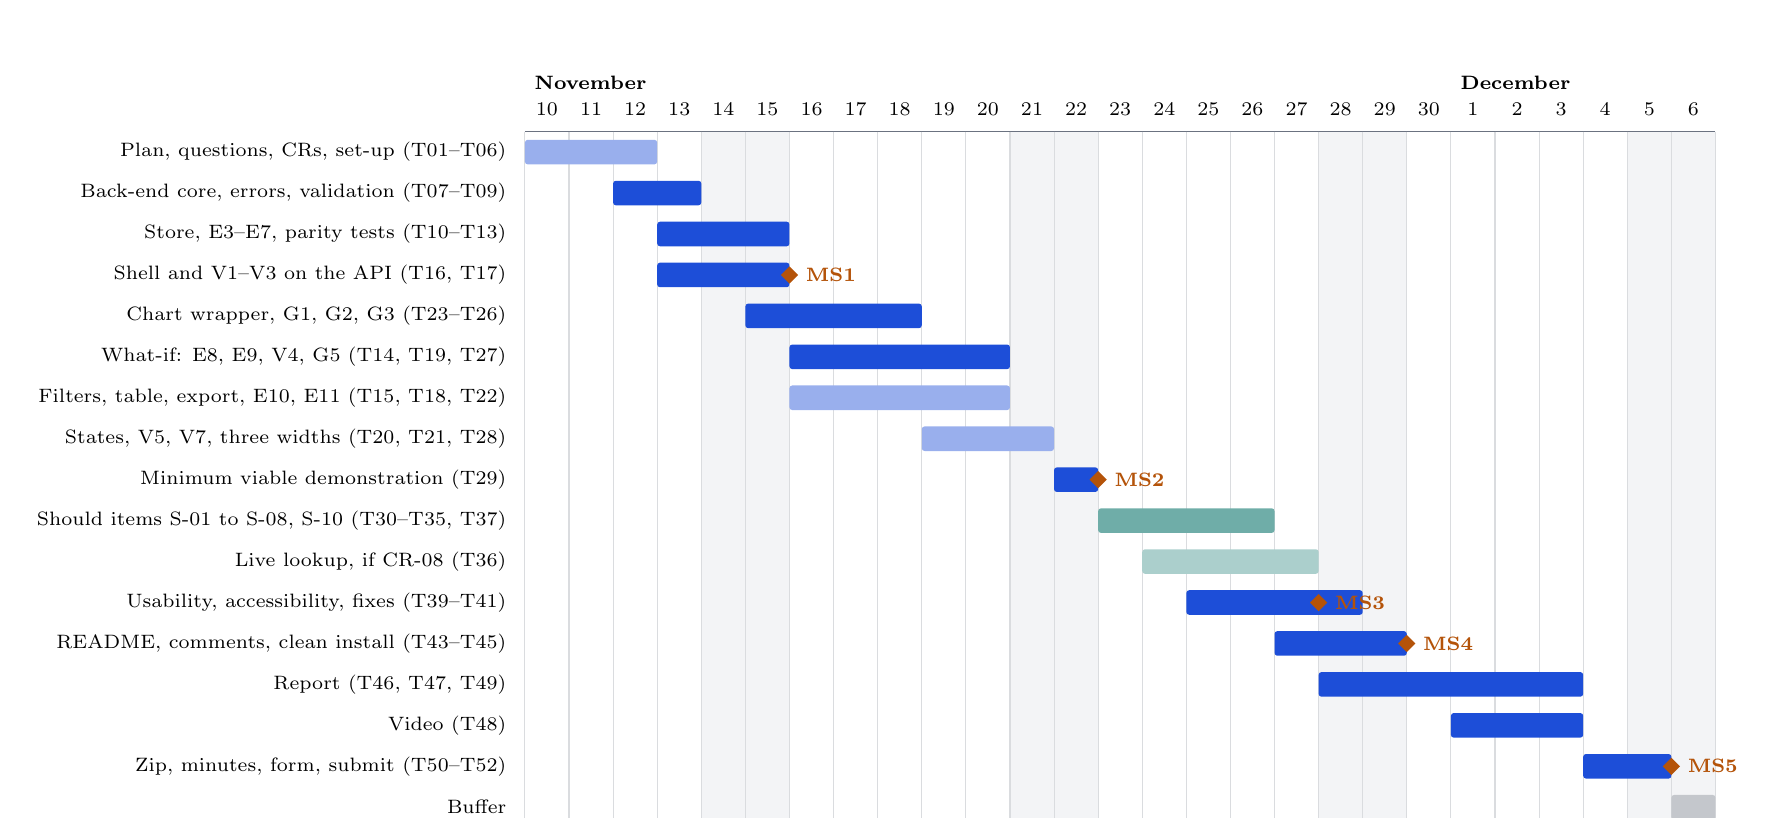
\begin{tikzpicture}[x=0.56cm, y=0.52cm, font=\scriptsize]
  % day columns: 0 = Tue 10 Nov ... 26 = Sun 6 Dec
  \def\labels{{"10","11","12","13","14","15","16","17","18","19","20","21","22","23","24","25","26","27","28","29","30","1","2","3","4","5","6"}}
  \def\nrows{17}
  \foreach \d in {0,...,26} {
    \pgfmathsetmacro{\lab}{\labels[\d]}
    \node[anchor=south] at (\d+0.5, 0.15) {\lab};
  }
  % weekends shaded
  \foreach \d in {4,5,11,12,18,19,25,26} { \fill[greysoft] (\d,0) rectangle (\d+1,-\nrows); }
  \node[anchor=south west, font=\scriptsize\bfseries] at (0,0.8) {November};
  \node[anchor=south west, font=\scriptsize\bfseries] at (21,0.8) {December};
  \draw[grey] (0,0) -- (27,0);
  \foreach \d in {0,...,27} { \draw[grey!25] (\d,0) -- (\d,-\nrows); }
  \newcommand{\task}[5]{%
    \node[anchor=east, align=right] at (-0.2, -#1+0.5) {#2};
    \fill[#5, rounded corners=1pt] (#3, -#1+0.2) rectangle (#4, -#1+0.8);
  }
  \newcommand{\mile}[3]{%
    \node[diamond, fill=warn, inner sep=1.6pt] at (#1, -#2+0.5) {};
    \node[anchor=west, font=\scriptsize\bfseries, text=warn] at (#1+0.15, -#2+0.5) {#3};
  }
  \task{1}{Plan, questions, CRs, set-up (T01--T06)}{0}{3}{accent!45}
  \task{2}{Back-end core, errors, validation (T07--T09)}{2}{4}{accent}
  \task{3}{Store, E3--E7, parity tests (T10--T13)}{3}{6}{accent}
  \task{4}{Shell and V1--V3 on the API (T16, T17)}{3}{6}{accent}
  \mile{6}{4}{MS1}
  \task{5}{Chart wrapper, G1, G2, G3 (T23--T26)}{5}{9}{accent}
  \task{6}{What-if: E8, E9, V4, G5 (T14, T19, T27)}{6}{11}{accent}
  \task{7}{Filters, table, export, E10, E11 (T15, T18, T22)}{6}{11}{accent!45}
  \task{8}{States, V5, V7, three widths (T20, T21, T28)}{9}{12}{accent!45}
  \task{9}{Minimum viable demonstration (T29)}{12}{13}{accent}
  \mile{13}{9}{MS2}
  \task{10}{Should items S-01 to S-08, S-10 (T30--T35, T37)}{13}{17}{teal!60}
  \task{11}{Live lookup, if CR-08 (T36)}{14}{18}{teal!35}
  \task{12}{Usability, accessibility, fixes (T39--T41)}{15}{19}{accent}
  \mile{18}{12}{MS3}
  \task{13}{README, comments, clean install (T43--T45)}{17}{20}{accent}
  \mile{20}{13}{MS4}
  \task{14}{Report (T46, T47, T49)}{18}{24}{accent}
  \task{15}{Video (T48)}{21}{24}{accent}
  \task{16}{Zip, minutes, form, submit (T50--T52)}{24}{26}{accent}
  \mile{26}{16}{MS5}
  \task{17}{Buffer}{26}{27}{grey!40}
\end{tikzpicture}}
\caption{Dark blue bars are on the critical path. Light blue bars have a day or two of float. Green
bars are the optional features, which can be cut without moving anything below them. Weekends are
shaded.}
\end{figure}

\subsection{Milestones and their gates}
\label{sec:milestones}

\begin{center}
\small
\begin{tabularx}{\textwidth}{@{}L{1.0cm}L{2.2cm}Y@{}}
\toprule
\textbf{No.} & \textbf{Date} & \textbf{Passed when} \\
\midrule
MS1 & Sun 15 Nov & Both tiers start from a fresh clone. E1 to E7 answer for all 28 addresses and pass the parity test. V1 to V3 show real data, with the unsupported and short-history states working \\
MS2 & Sun 22 Nov & The minimum viable demonstration of Section~\ref{sec:mvd}, on all 28 addresses, at three widths. Every Must item except M-14 to M-16 is done \\
MS3 & Fri 27 Nov & Feature freeze. Each Should item is either finished with its tests or cut and recorded. The walkthrough's issues rated 3 or 4 are fixed or have an owner and a date before MS4 \\
MS4 & Sun 29 Nov & Code freeze. The clean install passed on Windows and macOS. Both test suites pass. No error or warning at start or in the browser console. Tag \code{v1.0-rc}; only fixes after this \\
MS5 & Sat 5 Dec & The five files are on Canvas; the upload was downloaded and opened; the video link opens in a private window \\
\bottomrule
\end{tabularx}
\end{center}

\subsection{If the plan slips}
\label{sec:variance}

Assignment 1's rules (its §8.2) apply, with these dates:

\begin{itemize}
  \item \textbf{A task is late but its milestone holds.} The owner re-plans inside the week and
    says so in the team channel the same day.
  \item \textbf{MS1 is missed.} The Week 10 meeting moves people onto the late package. The Should
    tier shrinks by the same number of days, from the bottom of the cut order.
  \item \textbf{MS2 is missed.} It may move to Tuesday 24 November at most. Every day it moves
    removes a day of Should work; the live lookup goes first.
  \item \textbf{MS3 and MS4 do not move.} What is not finished is cut.
  \item \textbf{The submission date never moves.} If a due date is at risk, the tutor is told
    early; the tutor does not extend it.
\end{itemize}

\section{Risks, acceptance and the submission checklist}
\label{sec:risks}

\subsection{Risk register for Assignment 3}
\label{sec:riskregister}

The register continues the numbering, owners and scoring of Assignments 1 and 2. Risks that still
matter keep their number, with the trigger rewritten for this assignment; new risks start at 32.
The score is likelihood × impact with Assignment 1's mapping: Unlikely 1, Low 2, Moderate 3, Likely
and High 4; impact Low 2, Medium 3, High 4, Critical 5. Rows are sorted by score. The register is
reviewed at each weekly meeting and after each milestone.

{\small
\begin{longtable}{@{}L{0.7cm}L{3.2cm}L{2.0cm}L{3.4cm}L{4.6cm}@{}}
\toprule
\textbf{No.} & \textbf{Risk} & \textbf{L × I} & \textbf{Trigger / owner} & \textbf{Prevention; fallback} \\
\midrule
\endhead
7 & Critical-path tasks slip & Likely × Critical\newline 4×5 = 20 &
MS1 or MS2 missed; the work starts 13 days after Assignment 1's baseline / Le Quang Anh Hoang &
\textit{Prevention:} Must before Should; the contract frozen on day 59 so both tiers build at once;
a daily check against Section~\ref{sec:schedule}. \textit{Fallback:} cut from the bottom of
Section~\ref{sec:cutorder}; MS2 may move two days; the submission never moves. \\
9 & The code does not run on the marker's machine & Likely × High\newline 4×4 = 16 &
The clean install (T44) needs help, or anything prints a warning / Le Quang Anh Hoang &
\textit{Prevention:} pinned environments; start-up checks with one-sentence messages; Vite's proxy
so CORS never appears; two operating systems tested; expected output in the README.
\textit{Fallback:} the troubleshooting section and the pip route; tell the tutor at once. \\
32 & The rule on generative AI is broken or the use is under-declared & Moderate × Critical\newline 3×5 = 15 &
No written answer from the tutor by Fri 13 Nov; or a member cannot explain code they submitted /
Cam Dan Bui &
\textit{Prevention:} the question goes out on 11 Nov; \fp{docs/AI_USE_LOG.md} is kept daily; each
member owns an area and presents it in the video; the report acknowledges all use.
\textit{Fallback:} follow the tutor's ruling at once, re-plan who writes what, and declare
everything. \\
6 & Scope creep: optional features take time the Must tier needs & Likely × Medium\newline 4×3 = 12 &
Work on a Should or Could item while a Must item is open; a feature with no line in the change log /
Le Quang Anh Hoang &
\textit{Prevention:} the tiers; the MS2 gate; CR-07 and CR-08. \textit{Fallback:} stop the item and
record the cut in the minutes. \\
15 & Live API limits (only if CR-08 is approved) & Likely × Medium\newline 4×3 = 12 &
A 429 or a time-out during a lookup; any Must feature making a network call / Le Quang Anh Hoang &
\textit{Prevention:} off by default; a cache; two hosts; six lookups an hour; the video uses a
cached lookup and one short fresh one. \textit{Fallback:} switch the setting off; S-09 is cut and
nothing else changes. \\
33 & A library version makes the saved models warn or fail to load & Moderate × High\newline 3×4 = 12 &
A version message at start; a pickle error on another system / Cao Tri Tran &
\textit{Prevention:} Assignment 2's exact pins; a version and hash check at start; the same models
already ran on Windows, macOS and Linux in Assignment 2. \textit{Fallback:} the README's exact pip
command. The models are not re-saved (W-06). \\
36 & Uneven contribution, or a member cannot explain their part & Moderate × High\newline 3×4 = 12 &
A member with nothing merged by MS1; a dispute over the form's shares / Cam Dan Bui &
\textit{Prevention:} an area per member (Section~\ref{sec:wp}); reviews by a second member; the
minutes record who did what; the form's rule checked in Week 9. \textit{Fallback:} reassign packages
at the next meeting; tell the tutor early. \\
8 & The video cannot be opened, is corrupt, or runs over 7 minutes & Low × Critical\newline 2×5 = 10 &
The link is untested the day before; the rehearsal runs over 6:45 / Le Quang Anh Hoang &
\textit{Prevention:} a script and a timed rehearsal; a file and an unlisted link; a private-window
test by someone else; the link on the cover and in the text file. \textit{Fallback:} re-cut and
upload a second copy. \\
31 & Late or incomplete submission & Low × Critical\newline 2×5 = 10 &
Not submitted 24 hours before the deadline / Le Quang Anh Hoang &
\textit{Prevention:} the checklist of Section~\ref{sec:checklist}; submit on 5 December.
\textit{Fallback:} resubmit at once; if past the deadline, tell the tutor and submit anyway. \\
34 & The two tiers drift from the contract & Moderate × Medium\newline 3×3 = 9 &
A view fails on a real response that the mock accepted / Minh Khang Nguyen &
\textit{Prevention:} the freeze of T05; fixtures recorded from the real API; types generated from
the schema (S-10). \textit{Fallback:} the back end's schema wins; the client is fixed the same
day. \\
35 & The chart library slows loading or misbehaves on phones & Moderate × Medium\newline 3×3 = 9 &
The first chart is over budget; a touch gesture conflicts with scrolling / Minh Khang Nguyen &
\textit{Prevention:} a partial bundle loaded on demand; device checks at MS2.
\textit{Fallback:} a simpler tool bar; no WebGL; the table view always works. \\
40 & A bug found after the code freeze & Moderate × Medium\newline 3×3 = 9 &
A failing test or a review finding after MS4 / the package's owner &
\textit{Prevention:} both suites green before MS4; only fixes afterwards. \textit{Fallback:} fix,
retest, re-tag and rebuild the zip; re-record only the affected part of the video. \\
12 & A flag is read as proof of wrongdoing & Low × High\newline 2×4 = 8 &
A banned word, or a flag without the limitation line, anywhere; a walkthrough participant reads a
flag as guilt / Cao Tri Tran &
\textit{Prevention:} the wording tests on both tiers; views V5 and V7; the walkthrough's task 3.
\textit{Fallback:} fix the wording and retest with another participant. \\
37 & The Week 9--12 teaching expects a different stack detail & Low × Medium\newline 2×3 = 6 &
The tutor's answer to question 2 / Minh Khang Nguyen &
\textit{Prevention:} ask by 11 Nov; the README's commands are the same either way.
\textit{Fallback:} decide by 13 Nov, before front-end work is deep. \\
38 & The Assistant is too slow, or its weights cannot be shared & Moderate × Low\newline 3×2 = 6 &
An answer over 30 s on the PC; no agreed way to share 610 MB / Cao Tri Tran &
\textit{Prevention:} prepared answers; an optional download. \textit{Fallback:} the template only,
which is already the default. \\
39 & Canvas's size limits & Low × Medium\newline 2×3 = 6 &
The zip (about 40 MB) or the video is refused / Le Quang Anh Hoang &
\textit{Prevention:} question 3 to the tutor; a trial upload if Canvas allows drafts.
\textit{Fallback:} the unlisted link and the text file. \\
\bottomrule
\end{longtable}
}

\textbf{Earlier risks not carried forward:} those about Assignment 2's data, training and evaluation
(4, 13 and 23 to 30), which ended with its frozen results. Risk 13's rule still binds the wording:
no accuracy, precision or recall is ever claimed for real transactions, in the application or in the
report.

\subsection{Requirement traceability}
\label{sec:trace}

{\small
\begin{longtable}{@{}L{4.4cm}L{4.3cm}L{5.4cm}@{}}
\toprule
\textbf{Requirement (Assignment 1)} & \textbf{Built by} & \textbf{Verified by} \\
\midrule
\endhead
FR-01 select a supported address; coverage explained & V1; E3, E4; M-05, M-09 & AT-01, AT-02 \\
FR-02 timeline with range and source & V2; E5; G1 & AT-01 \\
FR-03 drilldown to a transaction's facts and source link & V3; E6, E7 & AT-05 \\
FR-04 reason, comparison basis and limitation line on every flag & V3; E7; \code{explorer.explain} & AT-03, AT-09 \\
FR-05 five distinguishable feedback states, each with a next action & The state catalogue (Section~\ref{sec:catalogue}) & AT-04 \\
DR-02 time-safe features & Assignment 2's package, unchanged; the batched what-if & The parity tests; AT-12 \\
NFR-01 units, source, snapshot date; no banned word; flags read as ``needs investigation'' & The chart contract; the wording tests; the walkthrough & AT-07, AT-09; walkthrough task 3 \\
NFR-02 another member can reproduce the set-up & README; pinned environments & AT-11 \\
NFR-03 keyboard, focus, contrast, recovery & Section~\ref{sec:a11y} & The accessibility inspection \\
AC-01, AC-02, AC-03 & J1, J3, J2 & AT-01, AT-02, AT-03 on every snapshot address \\
\bottomrule
\end{longtable}
}

\subsection{Acceptance tests}
\label{sec:acceptance}

Each is automated where it can be and repeated by hand for the test log.

{\small
\begin{longtable}{@{}L{1.1cm}L{9.6cm}L{3.4cm}@{}}
\toprule
\textbf{No.} & \textbf{Test} & \textbf{Covers} \\
\midrule
\endhead
AT-01 & For each of the 25 main addresses: chosen from V1, the overview shows the date range, labelled counts and a path to the flagged days & AC-01; FR-01, FR-02 \\
AT-02 & A valid address outside the snapshot gets the coverage explanation and three examples, and no result & AC-02 \\
AT-03 & Every flagged transaction's detail shows its contributing features with real values, the comparison basis and the limitation line (all flags through the API; three by hand) & AC-03; FR-04 \\
AT-04 & Invalid, unsupported, loading, empty, insufficient history and network failure each render with a next action & FR-05 \\
AT-05 & The facts of 20 random transactions equal the snapshot table, and each source link opens that transaction & FR-03 \\
AT-06 & A valid what-if returns eight verdicts; each invalid vector is refused in the browser and by the server; a too-early time answers 422 with a date that works & M-03, M-06, M-09 \\
AT-07 & Three or more chart types; each chart passes the contract's checklist; zoom, tooltip and click-through work & M-07; NFR-01 \\
AT-08 & The API uses GET and POST; its documentation lists every endpoint; each endpoint's errors answer as its row says & M-01, M-02 \\
AT-09 & No banned word in any response, view, state or export; the limitation line on every flag & NFR-01; risk 12 \\
AT-10 & J1 to J6 at 390, 820 and 1280 pixels with no sideways scrolling & M-11 \\
AT-11 & The README followed on Windows and on macOS by a member who did not write it, with no help, no error and no warning & M-14; risk 9 \\
AT-12 & For all 28 addresses the API returns what \code{Predictor} returns; each method's flags equal the scores table & M-02; DR-02 \\
\bottomrule
\end{longtable}
}

\subsection{Submission checklist}
\label{sec:checklist}

{\small
\begin{longtable}{@{}L{9.4cm}L{2.9cm}L{1.6cm}@{}}
\toprule
\textbf{Item} & \textbf{Who} & \textbf{By} \\
\midrule
\endhead
\multicolumn{3}{@{}l}{\textbf{Report}} \\
Eight pages or fewer by the script; cover has title, group, names, IDs, tutor and the video link & Cam Dan Bui & 3 Dec \\
All of the brief's sections; four or more endpoints documented in full; two diagrams & Cam Dan Bui & 3 Dec \\
Harvard references; every adapted figure cited; AI use acknowledged & Cam Dan Bui & 3 Dec \\
Wording check passes; every number comes from a script & Cao Tri Tran & 3 Dec \\
\multicolumn{3}{@{}l}{\textbf{Zip}} \\
Built from tag \code{v1.0}; \fp{SHA256SUMS.txt} verifies; no \fp{node_modules}, \fp{.git}, \fp{.env} or caches & Le Quang Anh Hoang & 4 Dec \\
Unzipped on a clean machine: the README's commands start both tiers; both test suites pass & Cam Dan Bui & 4 Dec \\
README has set-up, libraries, run steps for both tiers and the model's configuration & Le Quang Anh Hoang & 4 Dec \\
\multicolumn{3}{@{}l}{\textbf{Video}} \\
Under 7:00; MP4; sound clear; three device sizes; the whole workflow; decisions and difficulties & Minh Khang Nguyen & 3 Dec \\
Unlisted link opens in a private window on another member's machine; link on the cover and in the text file & Cam Dan Bui & 4 Dec \\
\multicolumn{3}{@{}l}{\textbf{Team documents}} \\
Minutes for Weeks 1 to 12, with CR-07 and CR-08 and the post-project review & Cam Dan Bui & 4 Dec \\
Contribution form checked against its rule and signed by all four & all & 4 Dec \\
\multicolumn{3}{@{}l}{\textbf{Upload}} \\
Five files with the group-name file names, uploaded by one member & Le Quang Anh Hoang & 5 Dec \\
Canvas receipt saved; the uploaded files downloaded again and opened & Le Quang Anh Hoang & 5 Dec \\
\bottomrule
\end{longtable}
}

\subsection{After submission}

\begin{itemize}
  \item The post-project review in the Week 12 minutes: what changed from this plan, and why.
  \item Kaggle tokens from Assignment 2 rotated; the archive folders on the PC deleted when marks
    are released.
  \item The repository stays private until marks are released; then the team decides whether to
    publish it beside Assignment 2's.
\end{itemize}


\appendix
\section{Change requests CR-07 and CR-08, and the messages to send}
\label{app:cr}

Assignment 1's §8.5 requires a change request to add an optional item from the scope exhibit, to
change a must-have item, or to use more than half of an assignment's buffer, and it needs every
member's agreement, at a meeting or by a recorded message within 48 hours. The fields follow the
Change Log (\fp{docs/change-log.md} since CR-06).

\subsection{CR-07: the Assignment 3 scope}

\begin{center}
\small
\begin{tabularx}{\textwidth}{@{}L{3.0cm}Y@{}}
\toprule
\textbf{Field} & \textbf{Entry} \\
\midrule
ID & CR-07 \\
Date raised & Tuesday 10 November 2026 \\
Requestor & Cao Tri Tran (Data/ML Lead) \\
Proposal & Adopt Section~\ref{sec:scope} of this plan as the scope of WBS 1.4. (1) Activate Assignment 1's optional items: a third chart type, zoom, filtering and tooltips, and CSV export. (2) Add to the must-have items: the what-if prediction and its form, the response curve, the models and limits page, export, and a health and a settings endpoint. (3) Add as optional items: the method selector, two more charts, the watchlist, the Assistant, the replay, linked selection, the scenario table, generated types and browser tests. (4) Record decisions D-A3-1 to D-A3-11 \\
Reason & The Assignment 3 rubric gives full points for three or more chart types, interactive charts, real-time updates and predictions from user input, and the brief's High Distinction list asks for at least three advanced functions. Assignment 1's minimum viable demonstration alone meets the brief's pass level \\
Impact on scope & Must items are added; nothing Assignment 1 promised is removed (Section~\ref{sec:promises}). Its five endpoints keep their shapes \\
Impact on schedule & WBS 1.4 starts on 10 November, 13 days after the baseline, and the new schedule (Section~\ref{sec:schedule}) uses the whole Assignment 3 buffer. Package 1.4.5 holds everything that can be cut \\
Impact on risk & Risks 6, 7, 8, 9, 12 and 31 are re-scored and risks 32 to 40 added (Section~\ref{sec:riskregister}) \\
Impact on quality & More evidence: tests on both tiers, a parity test against Assignment 2, a usability walkthrough, a clean install on two systems \\
Decision & Pending: approve, reject or defer, by name, at the Week 9 meeting \\
Changed artefacts & Scope exhibit; WBS dictionary 1.4.1 to 1.4.7; Gantt chart; risk register \\
\bottomrule
\end{tabularx}
\end{center}

\subsection{CR-08: a live lookup}

\begin{center}
\small
\begin{tabularx}{\textwidth}{@{}L{3.0cm}Y@{}}
\toprule
\textbf{Field} & \textbf{Entry} \\
\midrule
ID & CR-08 \\
Date raised & Tuesday 10 November 2026 \\
Requestor & Cao Tri Tran (Data/ML Lead) \\
Proposal & Allow the application, when a setting is on, to fetch the public confirmed history of any valid Bitcoin address from the Esplora API, score it with the frozen models and show it as live data (S-09, Section~\ref{sec:live}). The setting is off by default \\
Reason & The brief's High Distinction list names live data feeds, and the rubric's model line asks for real-time predictions on varied input. Assignment 2 already applies the frozen models to addresses outside the snapshot for its held-out test, with the same client \\
What it reverses & Assignment 1 §2.6: ``No live blockchain calls are made from the application''. Assignment 1's scope exhibit: addresses outside the curated sample are excluded \\
What it keeps & Every Must item reads local files (D-A3-7), so risk 15's trigger, ``the application needs a live call to run'', cannot fire. No identity, ownership or intent claim is made for any address; the wording rule and the limitation line apply to fetched addresses exactly as to snapshot ones \\
Impact on schedule & Four days of two members in package 1.4.5 (T36). First in the cut order after the tooling items \\
Impact on risk & Risk 15 is re-opened for S-09 only, with limits on rate, size and concurrency \\
Decision & Pending. Needed by Sunday 22 November; with no decision by then, S-09 is cut \\
\bottomrule
\end{tabularx}
\end{center}

\subsection{Message to the team}

\begin{summarybox}
\textbf{Assignment 3 plan and two change requests: please reply by Thursday's meeting.}

The delivery plan for Assignment 3 is in the repository (\fp{docs/A3_delivery_plan.pdf}). Sections
\ref{sec:summary} and \ref{sec:scope} are the ones to read first.

\textbf{CR-07.} Assignment 1's optional items (a third chart, zoom and filtering, CSV export) become
part of the build, and a what-if form, a response curve and a models page are added, because the
rubric's full points and the High Distinction list need them. Nothing from Assignment 1 is dropped.

\textbf{CR-08.} An optional live lookup of any Bitcoin address, off by default. It reverses
Assignment 1's ``no live calls'' statement, so it needs all four of us. If it is not approved by
22 November it is dropped and nothing else changes.

\textbf{Owners.} Section~\ref{sec:wp} proposes who builds what, following Assignment 1's WBS: Hoang
the back end, Khang the front end, Dan two charts, two views, the accessibility inspection and the
report, Cao the model layer. Say if you want a different split; each of us has to be able to explain
our part in the video.

Please reply ``approve'', ``reject'' or ``defer'' for each change request, by name.
\end{summarybox}

\subsection{Message to the tutor}

\begin{summarybox}
Dear Arthur,

We are starting Assignment 3 for group HCMC\_COS30049.1\_4 (the Bitcoin Address Activity Explorer)
and have six short questions.

\begin{enumerate}
  \item \textbf{Generative AI.} For Assignment 2 you allowed AI use with a separate declaration.
    The Assignment 3 brief says AI must not generate content, allows it for learning, idea
    generation and debugging, and asks for all use to be acknowledged in the report. Does the
    Assignment 2 arrangement still apply, and in what form would you like the acknowledgement?
  \item \textbf{Stack.} Our marked Assignment 1 prototype uses React with TypeScript and Vite. May
    we keep it in place of create-react-app?
  \item \textbf{Deadline and sizes.} Is the due time Sunday 6 December, 23:59 (GMT+7)? What are
    Canvas's size limits for the zip and for the video?
  \item \textbf{Model files.} The models the application needs are about 30 MB and are in the zip.
    An optional 152M language model is 610 MB. May the README link to it with a checksum?
  \item \textbf{Running it.} Is a local run from the README what you expect, or should it also be
    hosted somewhere?
  \item \textbf{API documentation.} May the complete API reference go in the appendix, with four
    endpoints documented in full inside the eight pages?
\end{enumerate}

Thank you. \\
Cao Tri Tran, for the group
\end{summarybox}

\section{Example requests and responses}
\label{app:json}

The values are real: they come from Assignment 2's \code{Predictor} at commit \code{aa56a26} for the
running example address. Numbers are shortened to four decimal places here; the API returns them in
full. Fields marked \emph{added} are not in Assignment 1's contract; \code{requestId} values are
illustrative.

\subsection{E4 \quad POST /api/lookup}

\begin{lstlisting}[style=json]
POST /api/lookup
{ "address": "1Bbcsfxj2JRUD5crcdZVHBcViT61vrJ3dz" }

200 OK
{ "status": "supported",
  "address": "1Bbcsfxj2JRUD5crcdZVHBcViT61vrJ3dz",
  "summary": { "address": "1Bbcsfxj2JRUD5crcdZVHBcViT61vrJ3dz",
               "firstSeen": "2024-05-16T05:16:19Z", "lastSeen": "2026-10-19T14:10:25Z",
               "txCount": 377, "scoredCount": 367, "flaggedCount": 3, "history": "sufficient",
               "kind": "p2pkh", "source": "snapshot" } }

400 Bad Request          (one character of the address changed)
{ "status": "invalid",
  "message": "This address fails its checksum, so it probably contains a typo.",
  "hint": "Bitcoin addresses start with 1, 3 or bc1. Check for a missing or extra character, or pick an address from the list.",
  "fields": [ { "name": "address", "message": "Checksum does not match." } ],
  "requestId": "0f3c9a1e7b2d" }

404 Not Found            (a valid address that is not in the snapshot)
{ "status": "unsupported",
  "message": "This address is not among the 28 addresses of the 22 October 2026 snapshot.",
  "examples": [ "36V7afbhZnvpMpBJmZf7XJKDeL2vtHDB6L", "3HTmUj5wFDQZ2TF8SAcngV7EQ88rptx35D",
                "35ZCxf5uyfc2VN194t8WRzz6RCEN6tQfmY" ],
  "canLookupLive": false,
  "requestId": "5a1d0c93e4f7" }
\end{lstlisting}

\subsection{E5 \quad GET /api/addresses/\{address\}/timeline}

\begin{lstlisting}[style=json]
GET /api/addresses/1Bbcsfxj2JRUD5crcdZVHBcViT61vrJ3dz/timeline

200 OK
{ "address": "1Bbcsfxj2JRUD5crcdZVHBcViT61vrJ3dz",
  "snapshot": { "snapshotDate": "2026-10-22", "source": "Blockstream Esplora",
                "sourceUrl": "https://blockstream.info/api", "illustrative": false,
                "dayTimeZone": "UTC", "addressCount": 28,
                "method": { "id": "baseline", "name": "Robust z baseline (A1)",
                            "flagAbsZ": 5.0, "contributingAbsZ": 2.0,
                            "note": "Flags mean unusual for this address's own history, nothing more." } },
  "range": { "start": "2024-05-16T05:16:19Z", "end": "2026-10-19T14:10:25Z" },
  "days": [ { "date": "2024-05-16", "txCount": 1, "flaggedCount": 0 },
            { "date": "2024-05-28", "txCount": 1, "flaggedCount": 0 },
            "... 214 days in all ..." ],
  "totals": { "txCount": 377, "scoredCount": 367, "flaggedCount": 3, "flaggedDays": 3 },
  "history": { "status": "sufficient", "txCount": 377, "spanDays": 886.3709,
               "required": { "minTx": 10, "minSpanDays": 14 },
               "firstScoredDate": "2024-07-11" } }
\end{lstlisting}

\subsection{E7 \quad GET /api/transactions/\{txid\}?address=}

\begin{lstlisting}[style=json]
GET /api/transactions/c91d9fbbd396070099f3147822cd6e1eb97b1de376ad353f42007149ddb73140
    ?address=1Bbcsfxj2JRUD5crcdZVHBcViT61vrJ3dz

200 OK
{ "txid": "c91d9fbbd396070099f3147822cd6e1eb97b1de376ad353f42007149ddb73140",
  "address": "1Bbcsfxj2JRUD5crcdZVHBcViT61vrJ3dz",
  "time": "2024-07-11T03:32:50Z", "blockHeight": 851629, "direction": "in",
  "receivedSats": 111260, "sentSats": 0, "netSats": 111260,
  "sourceUrl": "https://blockstream.info/tx/c91d9fbb...ddb73140",
  "scored": true, "flagged": true, "score": 5.6071,
  "method": { "id": "baseline", "name": "Robust z baseline (A1)", "flagAbsZ": 5.0,
              "contributingAbsZ": 2.0, "note": "Flags mean unusual for this address's own history, nothing more." },
  "features": [
    { "id": "F1", "name": "Size",          "value": 0.0011,  "usual": 0.0029,   "z": -2.8535, "role": "contributing" },
    { "id": "F2", "name": "Burst",         "value": 1.0,     "usual": 1.0,      "z":  0.0,    "role": "within-usual" },
    { "id": "F3", "name": "Gap",           "value": 47.9231, "usual": 144.1519, "z": -1.8129, "role": "within-usual" },
    { "id": "F4", "name": "Relative size", "value": 0.381,   "usual": 1.3857,   "z": -5.6071, "role": "flag" } ],
  "comparison": [
    { "features": ["F1", "F4"], "label": "Earlier transactions in the same direction",
      "description": "10 earlier transactions: the previous 30 days, extended back to reach 20",
      "txCount": 10, "start": "2024-05-16T05:16:19Z", "end": "2024-07-09T03:37:27Z" },
    { "features": ["F2", "F3"], "label": "All earlier transactions",
      "description": "10 earlier transactions: the previous 30 days, extended back to reach 20",
      "txCount": 10, "start": "2024-05-16T05:16:19Z", "end": "2024-07-09T03:37:27Z" } ],
  "limitation": "Unusual activity requires investigation; it does not indicate wrongdoing.",
  "explanation": "Flagged by Robust z baseline (A1).\nWhat stands out compared with this address's own history:\n- Lower ratio to the usual amount than usual: 0.4x the usual amount for this direction, against a usual 1.4x.\n- Smaller amount than usual: 0.0011126 BTC moved, against a usual 0.00291708 BTC.\nUnusual activity requires investigation; it does not indicate wrongdoing.",
  "scores": { "baseline": 5.6071, "isolation_forest": 0.5242, "lof": 1.465, "kmeans": 6.6898,
              "dbscan": 1.704, "regression": 2.5662, "regression_interval": -0.1636,
              "fusion": 0.9895, "txgpt_method": 5.5687 },
  "flags":  { "baseline": true, "isolation_forest": false, "lof": false, "kmeans": false,
              "dbscan": false, "regression": false, "regression_interval": false,
              "fusion": false, "txgpt_method": false },
  "source": "snapshot" }
\end{lstlisting}

Each feature also carries its \code{description}. \code{explanation}, \code{scores}, \code{flags}
and \code{source} are \emph{added}. This transaction is flagged by the baseline alone: a small
amount for this address, not a large one.

\subsection{E8 \quad POST /api/addresses/\{address\}/what-if}

\begin{lstlisting}[style=json]
POST /api/addresses/1Bbcsfxj2JRUD5crcdZVHBcViT61vrJ3dz/what-if
{ "amountBtc": 0.05, "direction": "out", "time": "2026-10-20T12:00:00Z" }

200 OK
{ "txid": "what-if", "address": "1Bbcsfxj2JRUD5crcdZVHBcViT61vrJ3dz",
  "time": "2026-10-20T12:00:00Z", "direction": "out",
  "receivedSats": 0, "sentSats": 5000000, "netSats": -5000000, "sourceUrl": null,
  "scored": true, "flagged": true, "score": 5.9755,
  "method": { "id": "baseline", "name": "Robust z baseline (A1)", "flagAbsZ": 5.0, "contributingAbsZ": 2.0 },
  "features": [
    { "id": "F1", "name": "Size",          "value": 0.05,    "usual": 0.000525, "z":  5.8804, "role": "flag" },
    { "id": "F2", "name": "Burst",         "value": 3.0,     "usual": 4.0,      "z": -0.4497, "role": "within-usual" },
    { "id": "F3", "name": "Gap",           "value": 21.8264, "usual": 10.0535,  "z":  0.3000, "role": "within-usual" },
    { "id": "F4", "name": "Relative size", "value": 95.2472, "usual": 0.9099,   "z":  5.9755, "role": "flag" } ],
  "comparison": [ { "features": ["F1", "F4"], "label": "Earlier transactions in the same direction",
                    "txCount": 20, "start": "2026-08-16T09:05:41Z", "end": "2026-10-08T09:34:20Z" },
                  { "features": ["F2", "F3"], "label": "All earlier transactions",
                    "txCount": 20, "start": "2026-09-15T01:02:36Z", "end": "2026-10-19T14:10:25Z" } ],
  "scores": { "baseline": 5.9755, "isolation_forest": 0.5565, "lof": 1.3138, "kmeans": 8.4075,
              "dbscan": 0.7390, "regression": 11.4714, "regression_interval": 0.4783, "fusion": 1.6388 },
  "flags":  { "baseline": true, "isolation_forest": false, "lof": false, "kmeans": false,
              "dbscan": false, "regression": true, "regression_interval": true, "fusion": true },
  "notAvailable": [ "txgpt_method" ],
  "explanation": "Flagged by Robust z baseline (A1).\nWhat stands out compared with this address's own history:\n- Higher ratio to the usual amount than usual: 95.2x the usual amount for this direction, against a usual 0.9x.\n- Larger amount than usual: 0.05 BTC moved, against a usual 0.00052495 BTC.\nUnusual activity requires investigation; it does not indicate wrongdoing.",
  "limitation": "Unusual activity requires investigation; it does not indicate wrongdoing.",
  "note": "A hypothetical transaction, compared with the address's real history before that time." }

400 Bad Request          { "amountBtc": 0, "direction": "sideways", "time": "tomorrow" }
{ "status": "invalid",
  "message": "Three values need correcting.",
  "fields": [ { "name": "amountBtc", "message": "Must be greater than 0." },
              { "name": "direction", "message": "Must be \"in\" or \"out\"." },
              { "name": "time", "message": "Use a date and time such as 2026-10-20T12:00:00Z." } ],
  "requestId": "c2e8b7d41a06" }

422 Unprocessable Entity { "amountBtc": 0.05, "direction": "out", "time": "2024-05-20T12:00:00Z" }
{ "status": "insufficient_history",
  "message": "At that time this address did not have enough earlier history to compare with.",
  "history": { "earlierTx": 1, "spanDays": 4.28, "required": { "minTx": 10, "minSpanDays": 14 } },
  "firstScoredDate": "2024-07-11",
  "requestId": "9b40e6a2f1c8" }
\end{lstlisting}

Four of the eight models flag this what-if: the baseline, both regression methods and the fusion.

\subsection{E9 \quad POST /api/addresses/\{address\}/what-if/curve}

\begin{lstlisting}[style=json]
POST /api/addresses/1Bbcsfxj2JRUD5crcdZVHBcViT61vrJ3dz/what-if/curve
{ "direction": "out", "time": "2026-10-20T12:00:00Z",
  "amountsBtc": [0.0001, 0.001, 0.01, 0.05, 0.1, 1, 10] }

200 OK
{ "address": "1Bbcsfxj2JRUD5crcdZVHBcViT61vrJ3dz", "direction": "out",
  "time": "2026-10-20T12:00:00Z", "usualBtc": 0.000525, "decidingMethod": "baseline",
  "amountsBtc": [0.0001, 0.001, 0.01, 0.05, 0.1, 1, 10],
  "methods": [
    { "id": "baseline", "name": "Robust z baseline (A1)", "threshold": 5.0,
      "scores": [2.1398, 0.9493, 3.9077, 5.9755, 6.8661, 9.8245, 12.7829],
      "flags":  [false, false, false, true, true, true, true] },
    "... seven more methods ..." ],
  "notAvailable": [ "txgpt_method" ] }
\end{lstlisting}

\subsection{Types the contract gains}

The prototype's \fp{src/api/types.ts} keeps every type it has. These are added; with S-10 they are
generated from the schema.

\begin{lstlisting}
export type MethodId = 'baseline' | 'isolation_forest' | 'lof' | 'kmeans' | 'dbscan'
  | 'regression' | 'regression_interval' | 'fusion' | 'txgpt_method';

export interface WhatIfRequest { amountBtc: number | string; direction: 'in' | 'out'; time: string; }

export interface ModelVerdicts {
  scores: Partial<Record<MethodId, number | null>>;
  flags: Partial<Record<MethodId, boolean>>;
  notAvailable?: MethodId[];
}

export interface WhatIfResult extends Omit<TransactionDetail, 'txid' | 'blockHeight'>, ModelVerdicts {
  txid: 'what-if';
  explanation: string;
  note: string;
}

export interface CurveResponse {
  address: string; direction: 'in' | 'out'; time: string;
  usualBtc: number | null; decidingMethod: MethodId; amountsBtc: number[];
  methods: { id: MethodId; name: string; threshold: number; scores: number[]; flags: boolean[] }[];
  notAvailable: MethodId[];
}

export interface FieldError { name: string; message: string; }
export interface ErrorExtras { hint?: string; fields?: FieldError[]; requestId?: string; }
\end{lstlisting}

\section{Commands}
\label{app:commands}

The order in which they are first needed. Paths are from the repository's root.

\subsection{Day one}

\begin{lstlisting}
# Assignment 2: tag the commit that was submitted (T02)
cd ../COS30049A2 && git tag a2-submitted <commit> && git push origin a2-submitted

# Assignment 3: copy the runtime with hashes (T03)
python tools/vendor_a2.py --from ../COS30049A2 --commit a2-submitted

# Back end (T03)
cd backend
conda env create -f environment.yml
conda activate cos30049-a3
python -m pytest -q

# Front end (T04)
cd ../frontend
npm install
npm test
\end{lstlisting}

\subsection{Every day}

\begin{lstlisting}
# terminal 1
cd backend && conda activate cos30049-a3
uvicorn app.main:app --reload --port 8000        # API documentation at http://localhost:8000/docs

# terminal 2
cd frontend && npm run dev                       # the application at http://localhost:5173

# before every commit: both must exit with code 0
cd backend  && python -m pytest -q
cd frontend && npm run typecheck && npm run lint && npm test
\end{lstlisting}

\subsection{Checks by hand}

\begin{lstlisting}
curl http://localhost:8000/api/health
curl http://localhost:8000/api/addresses
curl http://localhost:8000/api/addresses/1Bbcsfxj2JRUD5crcdZVHBcViT61vrJ3dz/timeline
curl -X POST http://localhost:8000/api/addresses/1Bbcsfxj2JRUD5crcdZVHBcViT61vrJ3dz/what-if \
     -H "Content-Type: application/json" \
     -d '{"amountBtc": 0.05, "direction": "out", "time": "2026-10-20T12:00:00Z"}'
\end{lstlisting}

On Windows' Command Prompt the last command needs double quotes around the body with the inner
quotes escaped; the README gives both forms, and the documentation page at \code{/docs} can send
the same request from the browser.

\subsection{Tooling}

\begin{lstlisting}
python tools/export_openapi.py                   # writes backend/openapi.json (committed; the report reads it)
npm run fixtures                                 # refreshes the mock's answers from the running back end
npm run types                                    # S-10: TypeScript types from openapi.json
npm run screenshots                              # three widths; fails on sideways scrolling
npx playwright test                              # S-11: the journeys in three browsers
python tools/measure.py                          # S-12: the measured performance table
python tools/precompute_assistant.py             # S-05: guarded answers for the snapshot's flags (needs the weights)
\end{lstlisting}

\subsection{Freeze and package}

\begin{lstlisting}
git tag v1.0-rc                                  # MS4, after the clean install
git tag v1.0                                     # Fri 4 Dec
python tools/package.py --tag v1.0               # dist/HCMC_COS30049.1_4_Assignment3_Code.zip and SHA256SUMS.txt
# then, in an empty folder on a clean machine: unzip, follow the README, run both test suites
\end{lstlisting}

\subsection{This plan}

\begin{lstlisting}
cd docs/plan
pdflatex main && pdflatex main && pdflatex main
cp main.pdf ../A3_delivery_plan.pdf
\end{lstlisting}


\end{document}
